\documentclass[10.5ptj,a4j,dvipdfmx,uplatex, oneside, openany, report]{jsbook}%ここのdraft消すと画像が出る

% レイアウト
\usepackage[driver=dvipdfm,hmargin=19.05truemm,vmargin=25.40truemm]{geometry}

% エンコーディング
\usepackage[T1]{fontenc}

% 日本語フォント
\usepackage[expert,deluxe,uplatex]{otf}

% 数式・科学表記
\usepackage{amsmath,amssymb,bm,mleftright,diffcoeff}
\usepackage{siunitx}


\usepackage{comment}

% 画像処理
\usepackage[dvipdfmx]{graphicx}

% 参考文献スタイル指定
\usepackage[nobreak]{cite}
\usepackage[resetlabels]{multibib}
\newcites{pubs}{発表文献}
\bibliographystyle{junsrt} %jplain
\bibliographystylepubs{junsrt}
\nocitepubs{*}

% 相互参照
\usepackage[hidelinks]{hyperref}

% URL
\usepackage{url}

% 画像用ディレクトリ
\graphicspath{{images/}}

%%
%% タイトル・著者・日付
%%
\usepackage{dendentitle}
\title{歌唱発声における発声難度の音高・音色依存性に関する\\分析的検討}
\author{電気電子工学科 03-180480  小林海斗}
\date{2020/2/7}

%%
%% main
%%
\begin{document}
\maketitle

\tableofcontents

\chapter{序論}

\section{研究の背景}
自然な歌唱は

従来の研究としては
宋らの研究では調音運動に基づいて発声難度を求め、それを歌詞自動生成の指標として用いている\cite{so}。
また、佐藤らの研究では調音運動に加えて音響特徴量に着目し、日本語単語の発声しやすさを評価している\cite{sato}。
しかしこれらは調音的な側面が強く、歌声の要素の一つである音高による影響が考慮されていない。


\section{研究の目的}
本研究では、音声合成や歌詞作成などへの応用のために発声難度の音高・音色依存性を分析することを目的とする。
使用する音声データは被験者による母音に限定した歌声を収録したものを用いる。得られるデータに対して分析を行い、
音高・音色依存性を探る。
また、収録プロトコルを確立することで今後の発声難度分析の一助となることも本研究の目的である。

\section{本論文の構成}
本論文は全6章で構成される。
第2章では、日本語単語における発声しやすさの自動評価に関する先行研究と、$F_0$動的変動成分に関する先行研究について述べる。
第3章では、本研究で用いる$F_0$抽出の理論的背景、母音と構音の関係について述べる。
第4章では、収録実験の詳細と得られたデータに対する客観的評価について述べる。
第5章では、得られたデータに対して行った分析、およびその分析から導かれる発声難度への影響要素について述べる。
そして第6章では、結論と今後の課題について述べる。



\chapter{関連研究}


\section{日本語単語における発声しやすさの自動評価}
佐藤らは、日本語単語の発声難度を識別するための特徴量として調音データから抽出した特徴量と音声データから抽出した特徴量に一定の有効性があることを示した\cite{sato}。

\subsection{調音運動及び音響特徴量に着目した特徴量の提案}
発話の長さが異なる場合、フレーム分割による特徴量抽出は次元が合わずそのまま比較できないため、ここでは
表\ref{table:expected}の特徴量を用いている。

\begin{table}[h]
    \small
    \caption{発声しにくさの指標として機能することを期待する特徴量}
    \label{table:expected}
    \centering
    \begin{tabular}{ccc}
        \hline
        タグ & 抽出する特徴量 & 次元数 \\
        \hline \hline
        articulation-based1 & 
        \begin{tabular}{c}
            12次元の調音データの各次元の時系列\\データに対する平均、ケプストラムの先\\頭12次元 
        \end{tabular}  
        & 156\\
        articulation-based2 & 
        \begin{tabular}{c}
            \\2次元の調音データの各次元の時系列\\データ、時系列データの一次微分、二次\\微分それぞれに対する平均、分散、最大\\値、最小値、最小二乗法によって一次関\\数、二次関数に近似した際の係数および\\近似誤差
        \end{tabular}  
        & 396\\
        cepstrum-based & 
        \begin{tabular}{c}
            \\音声データのケプストラム、$\Delta$特徴量、\\$\Delta\Delta$特徴量各13次元に対する平均、分\\散、最大値、最小値、最小二乗法によっ\\て一次関数、二次関数に近似した際の係\\数および近似誤差 
        \end{tabular}  
        & 429\\
        mfcc-based & 
        \begin{tabular}{c}
            \\音声データのMFCC、$\Delta$特徴量、$\Delta\Delta$特\\徴量各13次元に対する平均、分散、最大\\値、最小値、最小二乗法によって一次関\\数、二次関数に近似した際の係数および\\近似誤差 
        \end{tabular}      
        & 429\\
        \hline
    \end{tabular}
\end{table}

\subsection{作成データセットを用いた発声しやすさの識別}
主観実験で得られたデータに対し、表\ref{table:expected}の特徴量を用いてサポートベクターマシンによって分類を行う。

ラベルは2種類作成している。単語に付与された5段階スコアをもとに、スコア3.0を境界として発声難度を定める方式(with inntermediate: w/ mid)と、スコア2.0以下と4.0以上のみを用いる方式(without inntermediate: w/o mid)である。
後者は中間スコアを含まず、主観評価がより安定しているもののみを識別に用いているといえる。

これによる正解率、適合率、再現率、F値を示したものを表\ref{table:SVM}に示す。
w/ midでは正解率は70\%前後で特徴量による大きな差はなかったが、w/o midでは全ての特徴量で正解率が上がり、音響特徴量に基づくcepstrum-based、mfc-basedが特に高い正解率を示した。

\begin{table}[h]
    \small
    \caption{データセットを用いたSVMによる分類}
    \label{table:SVM}
    \centering
\begin{tabular}{cccccc}
    \hline
    ラベリング & 特徴量 & 正解率 & 適合率 & 再現率 & F値\\
    \hline \hline
    w/ mid & articulation-based1 & 62.9\% & 38.7\% & 33.3\% & 35.8\%\\
    & articulation-based2 & 75.0\% & 59.5\% & 61.1\% & 60.3\%\\
    & cepstrum-based & 72.4\% & 56.3\% & 50.0\% & 52.9\%\\
    & mfcc-based & 70.7\% & 52.8\% & 52.8\% & 52.8\%\\
    \hline
    w/o mid & articulation-based1 & 75.4\% & 47.1\% & 53.3\% & 50.0\%\\
    & articulation-based2 & 75.4\% & 47.3\% & 60.0\% & 52.9\%\\
    & cepstrum-based & 90.8\% & 75.5\% & 86.7\% & 81.3\%\\
    & mfcc-based & 81.5\% & 57.9\% & 73.3\% & 64.7\%\\
    \hline

\end{tabular}
\end{table}

\section{歌声特有の$F_0$動的変動成分}
齋藤らは様々な歌声データの$F_0$変化パターンを分析し、以下に示す4種類の$F_0$動的変動成分が歌唱スタイルや歌唱者に関係なく
存在することを明らかにした\cite{singbyspeaking}。
\begin{description}
    \item[オーバーシュート(Overshoot)]滑らかな音高変化、およびその直後に目的音高を超える瞬時的な変動成分
    \item[ヴィブラート(Vibrato)]同一音高区間で観測される4〜8Hzの準周期的な変動成分
    \item[プレパレーション(Preparationn)]音高の変化直前に変化とは逆方向に触れる瞬時的な変動成分
    \item[微細振動(Fine fluctuation)] 発声区間全体に観測される15〜20Hz程度の不規則で細かい変動成分
\end{description}

図\ref{f0_moving}はアマチュア歌手による日本童謡「七つの子」の$F_0$変化パターンおよび$F_0$動的変動成分である。
これから上記の微細振動を除く変動成分が生じていることが読み取れる。

\begin{figure}[htbp]
    \begin{center}
      \includegraphics[clip,width=12.0cm]{f0_moving.png}
      \caption{アマチュア歌唱者の歌声における$F0$動的変動成分の例\cite{singbyspeaking}}
      \label{f0_moving}
    \end{center}
\end{figure}

このような$F0$動的変動成分は歌声を知覚する上で重要な役割を担っており、自然な歌声合成の要素の一つとして応用が可能であると考えられる。



%---------------------------%

\chapter{理論的背景}
\section{母音とフォルマント周波数}
フォルマント周波数は母音や声質の決定において非常に重要である。
フォルマント周波数は声道スペクトルのピークとなる共鳴周波数のことであり、
低い方から順に第1フォルマント($F_1$)、第2フォルマント($F_2$)、と名付けられる。

調音器官の運動は、フォルマント周波数全てに影響を与える。
第1フォルマントは顎の開きに敏感で、開き具合が大きくなるほど第1フォルマント周波数は上昇する。
第2フォルマントは特に舌の形状に大きく影響を受け、声道前方を狭めるときに第2フォルマント周波数はもっとも高くなる。
逆に、軟口蓋や咽頭部を狭める時には低くなる。
第3フォルマントは舌尖の位置、正確には前歯のすぐ後ろの空間に影響を受け、空間が大きいほど第3フォルマント周波数は低くなる。

フォルマント周波数のうち特に$F_1$、$F_2$は母音を特徴付ける重要なパラメータであり、これらの分布によって母音を分類することができる\cite{japanese_vowels}。
図\ref{jp_formant}は日本語5母音における$F_1$、$F_2$を示したものである。

\begin{figure}[htbp]
    \begin{minipage}{0.5\hsize}
        \begin{center}
            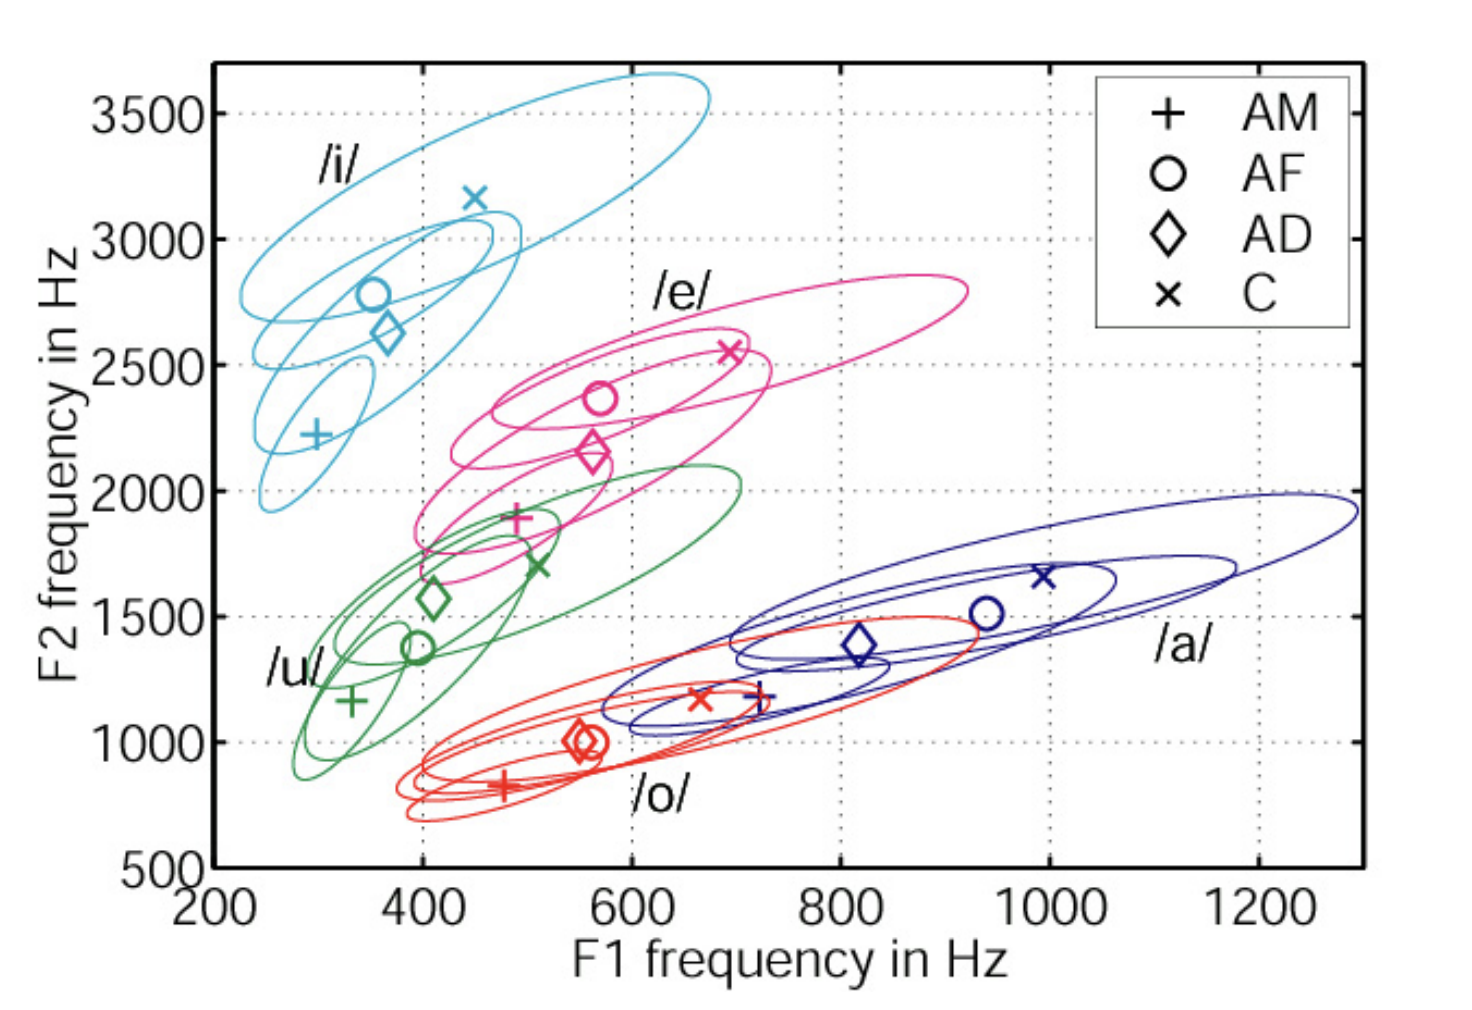
\includegraphics[clip,width=7.0cm]{5母音.png}
            \caption{日本語5母音の$F_1$、$F_2$\cite{japanese_vowels}}
            \label{jp_formant}
        \end{center}
    \end{minipage}
    \begin{minipage}{0.5\hsize}
        \begin{center}
            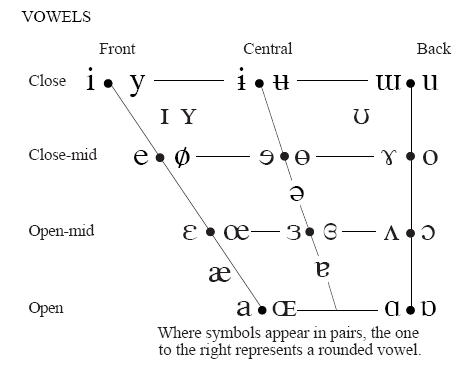
\includegraphics[clip,width=7.0cm]{vowels.png}
            \caption{IPA母音チャート}
            \label{vowels}
        \end{center}
    \end{minipage}
\end{figure}

ここでAMは成人男性、AFは成人女性、ADは青年、Cは子供である。一般に、平均的な声が高いほど
フォルマント周波数も高い傾向にある。
成人男性を例に挙げると、$F_1$は250〜1000 \si{Hz}、$F_2$は600〜2500 \si{Hz}、
$F_3$は1700〜3500 \si{Hz}である\cite{science}。


また、図\ref{vowels}はIPAが定めた母音チャートである\footnote{https://www.internationalphoneticassociation.org/content/ipa-vowels}。
縦軸は口の開き具合に対応し、上に行くほど狭くなる。
横軸は舌の前後位置に対応し、左に行くほど前寄りである。
これは適切に反転と回転を行うことで図\ref{jp_formant}と重なることが知られている。





%---------------------------%


\chapter{音高・音色における発声難度の調査}

歌唱能力は個人差に依るところが大きいが、全体としておおまかな発声難度の傾向はあると考えられる。
一般には/i/の母音では高音域が出しにくいとされている。
女性は男性と比較してフォルマント周波数が高く、音域も異なることから同時に傾向を掴むのは難しいと考え、ここでは男性に限定して調査を行う。
男性の地声と裏声の声区の重複する区間は200〜350Hz(G3〜F4)であるが、この声区の幅、境界は個人により大きく異なる。
そのため、使用音域は男性の平均的な地声の範囲に収まるように設定した。

\section{実験条件}
\begin{description}
    \item[被験者]\mbox{}\\
        実験は20代男性4人を対象として行った。
    \item[収録音声]\mbox{}\\
        発声は/a/、/i/、/u/、/e/、/o/を用いた。
        音高は平均律におけるF3(174.6Hz)、A3(220.0Hz)、C4(261.6Hz)、A4(440.0Hz)の4音を使用した。
        サンプリング周波数は44100Hzで、モノラル形式で収録を行った。
    \item[実験内容]\mbox{}\\
        実験内容は以下に示す通りである。
        \begin{description}
            \item[共通項目]\mbox{}\\
                ・全てテンポ120で行う。
                
                ・各実験はそれぞれ2回ずつ行う。
                
                ・初めに音源を流しながら発声練習する時間を設け、発声に慣れたことが確認でき次第収録を開始する。

                ・発声後に、発声難度を主観で評価する。この評価は「発声しにくい」「どちらとも言えない」「発声しやすい」の3段階で行う。
                
                ・収録と同時に、正面から発声時の口部の様子を録画する。
            \item[単音]\mbox{}\\
                8拍(4秒)のカウントの後、/a/の発声でF3の音高を16拍(8秒)伸ばした後8拍(4秒)休憩する。
                これを音高をA3、C4、F4と変えて行う。
                発声を/i/、/u/、/e/、/o/に変えた場合においても同様に行う。
                発声が5通り、音高が4通りで合計20回収録する。
            \item[上昇]\mbox{}\\
                4拍(2秒)のカウントの後、/a/の発声でF3の音高を2拍(1秒)伸ばし、その後/a/の発声でA3の音高を2拍(1秒)
                伸ばす。
                これを、後半の音高A3をC4、F4と変えて行う。
                前後の発声を/i/、/u/、/e/、/o/に変えた場合においても同様に行う。
                発声が25通り、音高変化が3通りで合計75回収録する。
            \item[下降]\mbox{}\\
                4拍(2秒)のカウントの後、/a/の発声でA3の音高を2拍(1秒)伸ばし、その後/a/の発声でF3の音高を2拍(1秒)伸ばす。
                これを、前半の音高A3をC4、F4と変えて行う。
                前後の発声を/i/、/u/、/e/、/o/に変えた場合においても同様に行う。
                発声が25通り、音高変化が3通りで合計75回収録する。
        \end{description}

    \item[使用機材]\mbox{}\\
        使用機材を表\ref{table:items}に示す。
        \begin{table}[h]
            \caption{使用機材}
            \label{table:items}
            \centering
            \begin{tabular}{clll}
                \hline
                使用機材 & 型番 \\
                \hline \hline
                コンデンサマイク & SONY C-48\\
                ヘッドフォン & SONY MDR-CD480\\
                レコーダ & KORG MR-1000\\
                カメラ & SONY FDR-AX45\\
                \hline
            \end{tabular}
        \end{table}
        
\end{description}








\section{実験結果}
以下に被験者1の実験結果を示す。他の被験者の結果は付録に載せている。
$F_0$抽出には音声合成システムWORLD\cite{world}のHarvest\cite{harvest}を用いた。
Harvestは図\ref{harvest}のように$F_0$候補の推定部と推定された$F_0$候補から軌跡を生成する部からなる
ピッチ抽出手法であり、他の手法と比較して耐雑音性が高いことで知られている。
なお、$F_0$間隔は1msである。

\begin{figure}[htbp]
    \begin{center}
      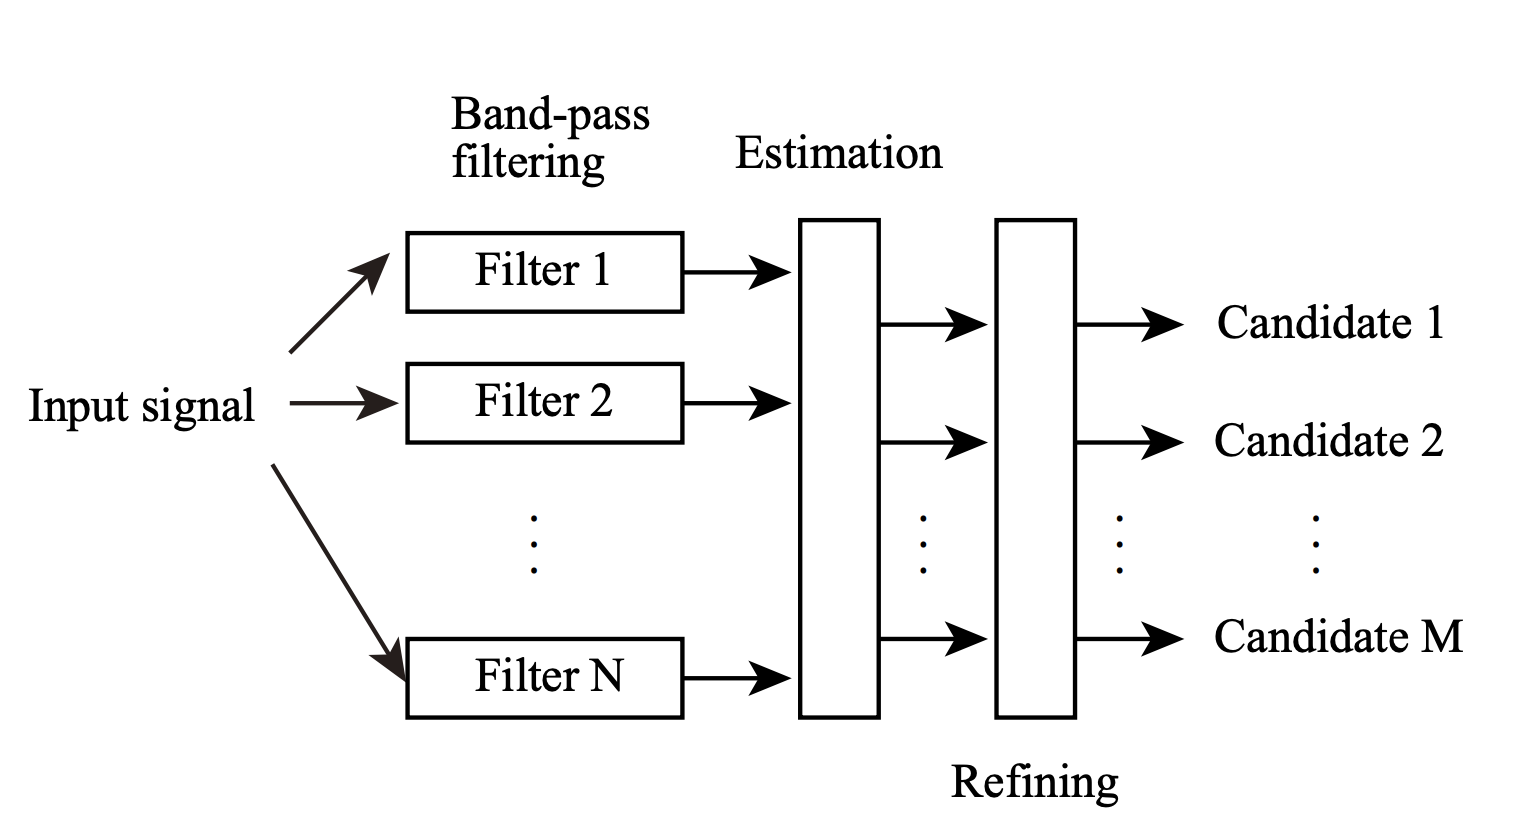
\includegraphics[clip,width=7.0cm]{harvest.png}
      \caption{Harvestによる$F_0$候補推定の流れ\cite{harvest}}
      \label{harvest}
    \end{center}
\end{figure}

\subsection{単音}
被験者1の単音発声の$F_0$軌跡を図\ref{la}、\ref{li}、\ref{lu}、\ref{le}、\ref{lo}に示す。
歌い出しで音高が外れてしまっている場合でも、1秒以内に正しい音高に近い音高で発声を修正できている。
また、歌い終わりは息が持たなかったために早めに切ってしまった音声が存在している。


\begin{figure}[htbp]
    \begin{minipage}{0.33\hsize}
        \begin{center}
            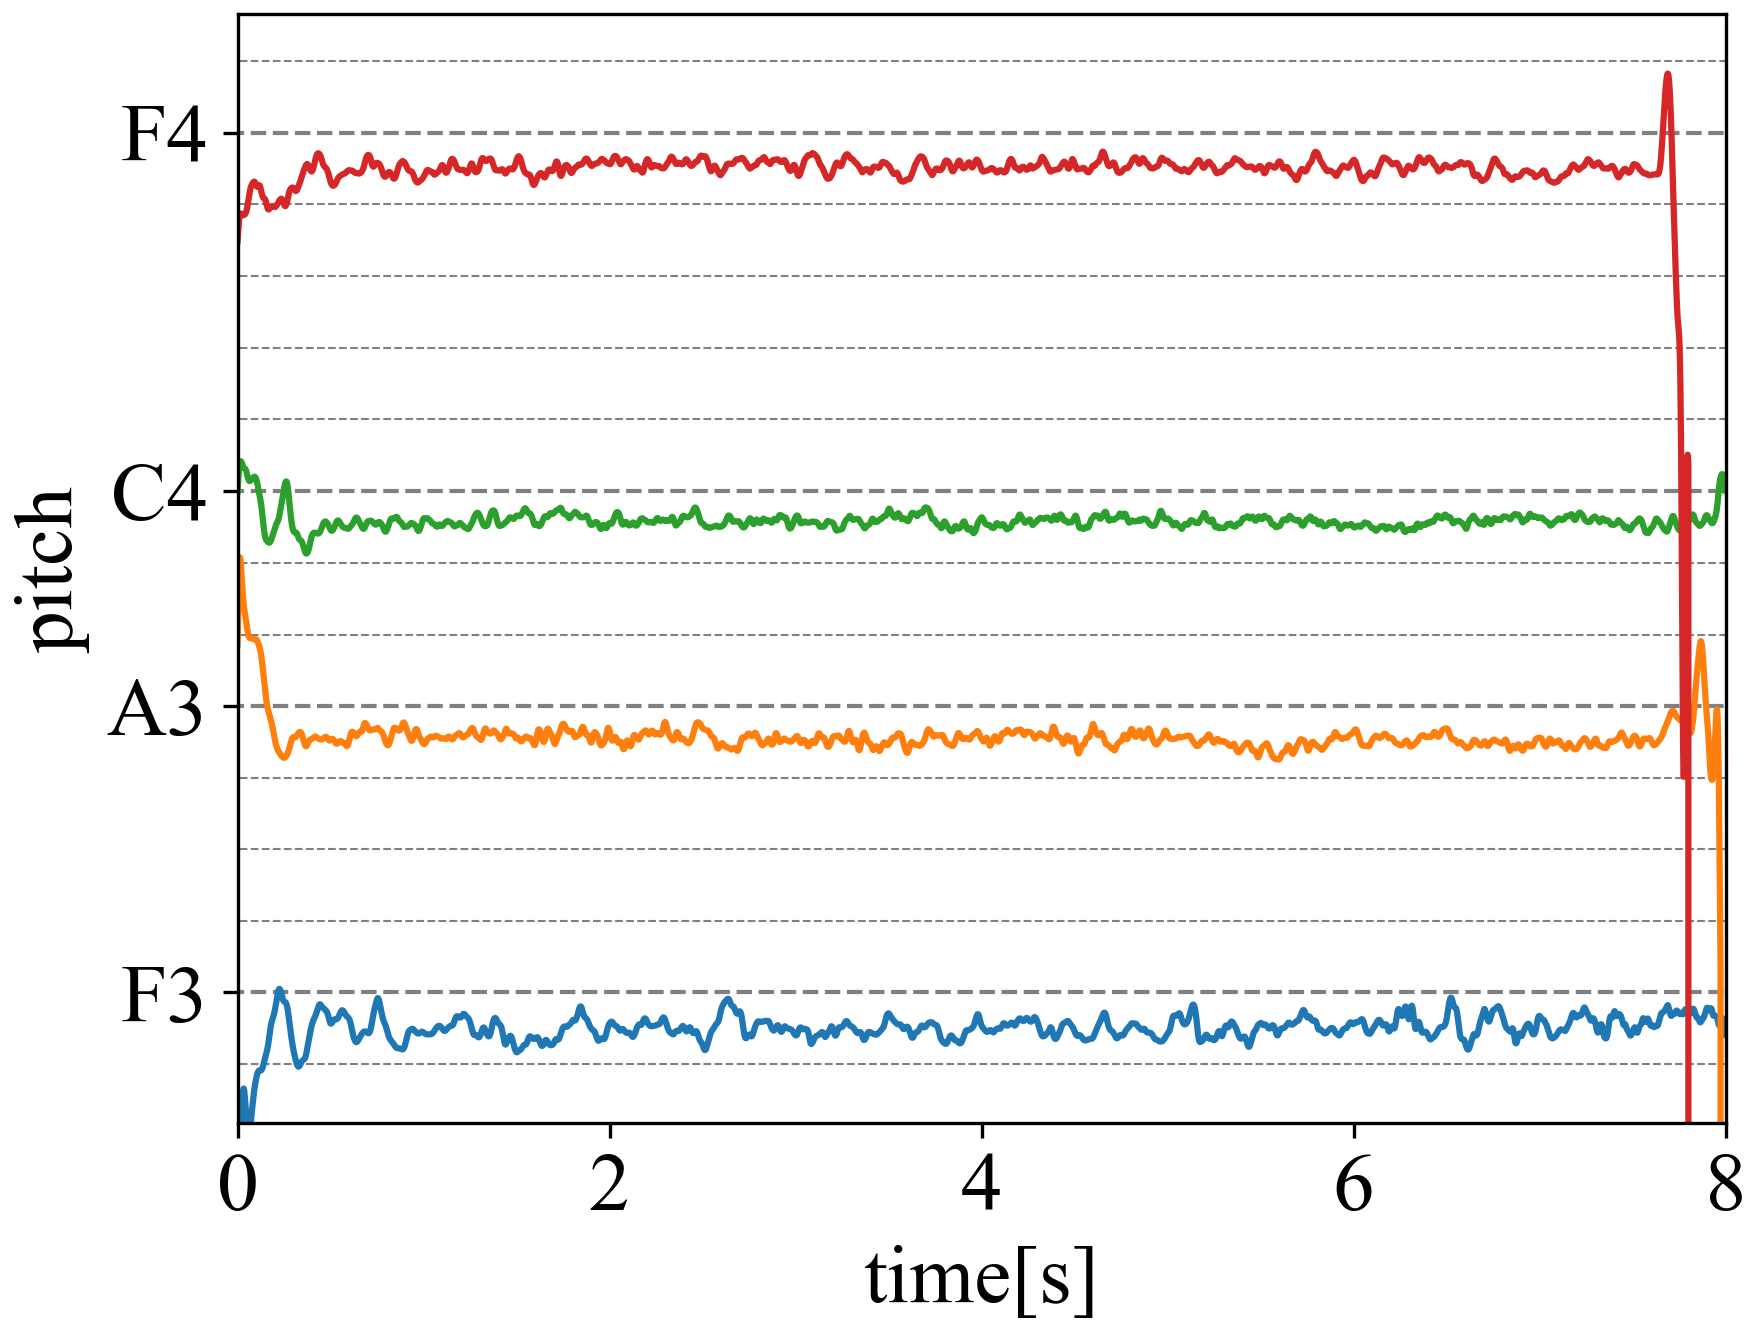
\includegraphics[width=5cm]{long/long_1_a.png}
            \caption{被験者1の/a/単音発声}
            \label{la}
        \end{center}
    \end{minipage}
    \begin{minipage}{0.33\hsize}
        \begin{center}
            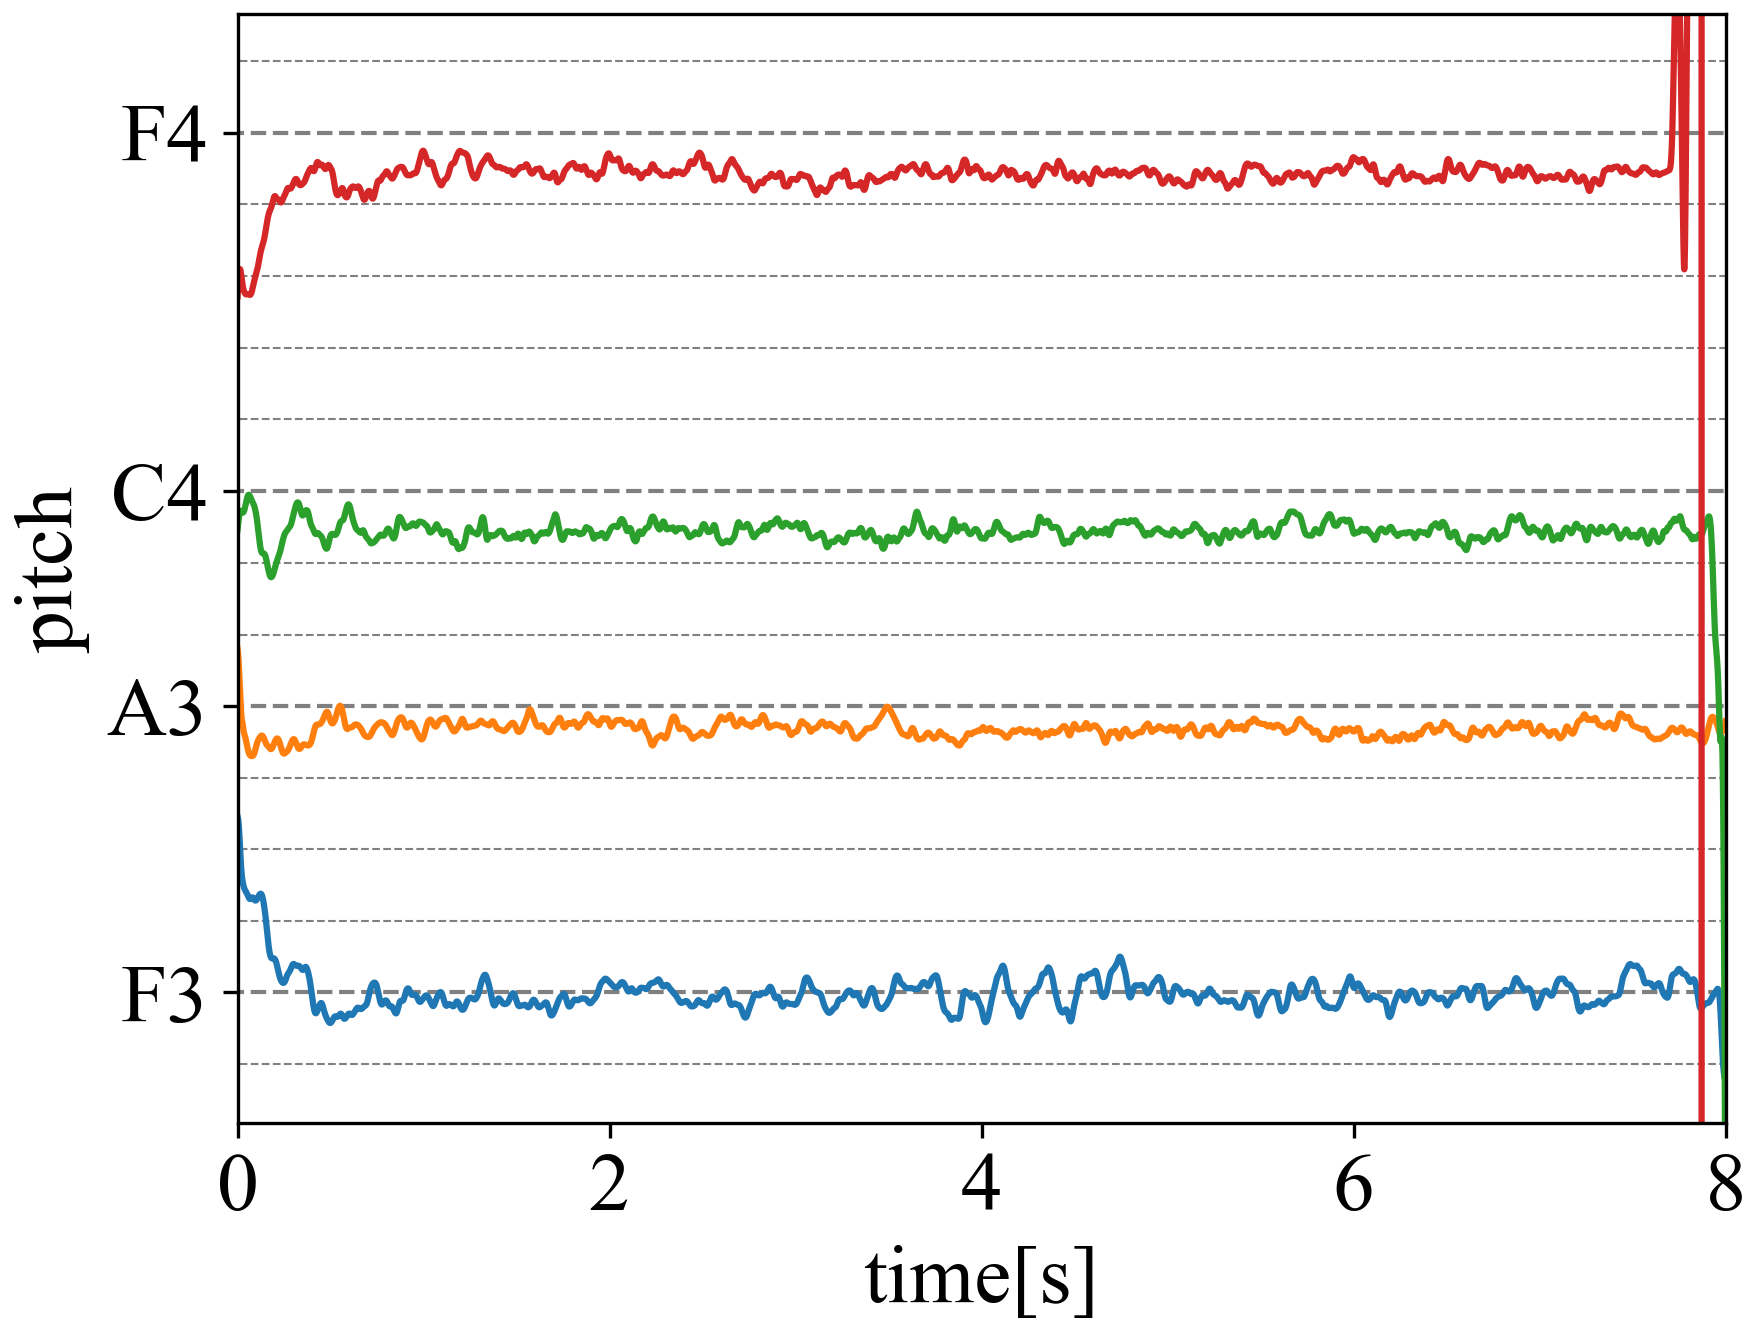
\includegraphics[width=5cm]{long/long_1_i.png}
            \caption{被験者1の/i/単音発声}
            \label{li}
        \end{center}
    \end{minipage}
    \begin{minipage}{0.33\hsize}
        \begin{center}
            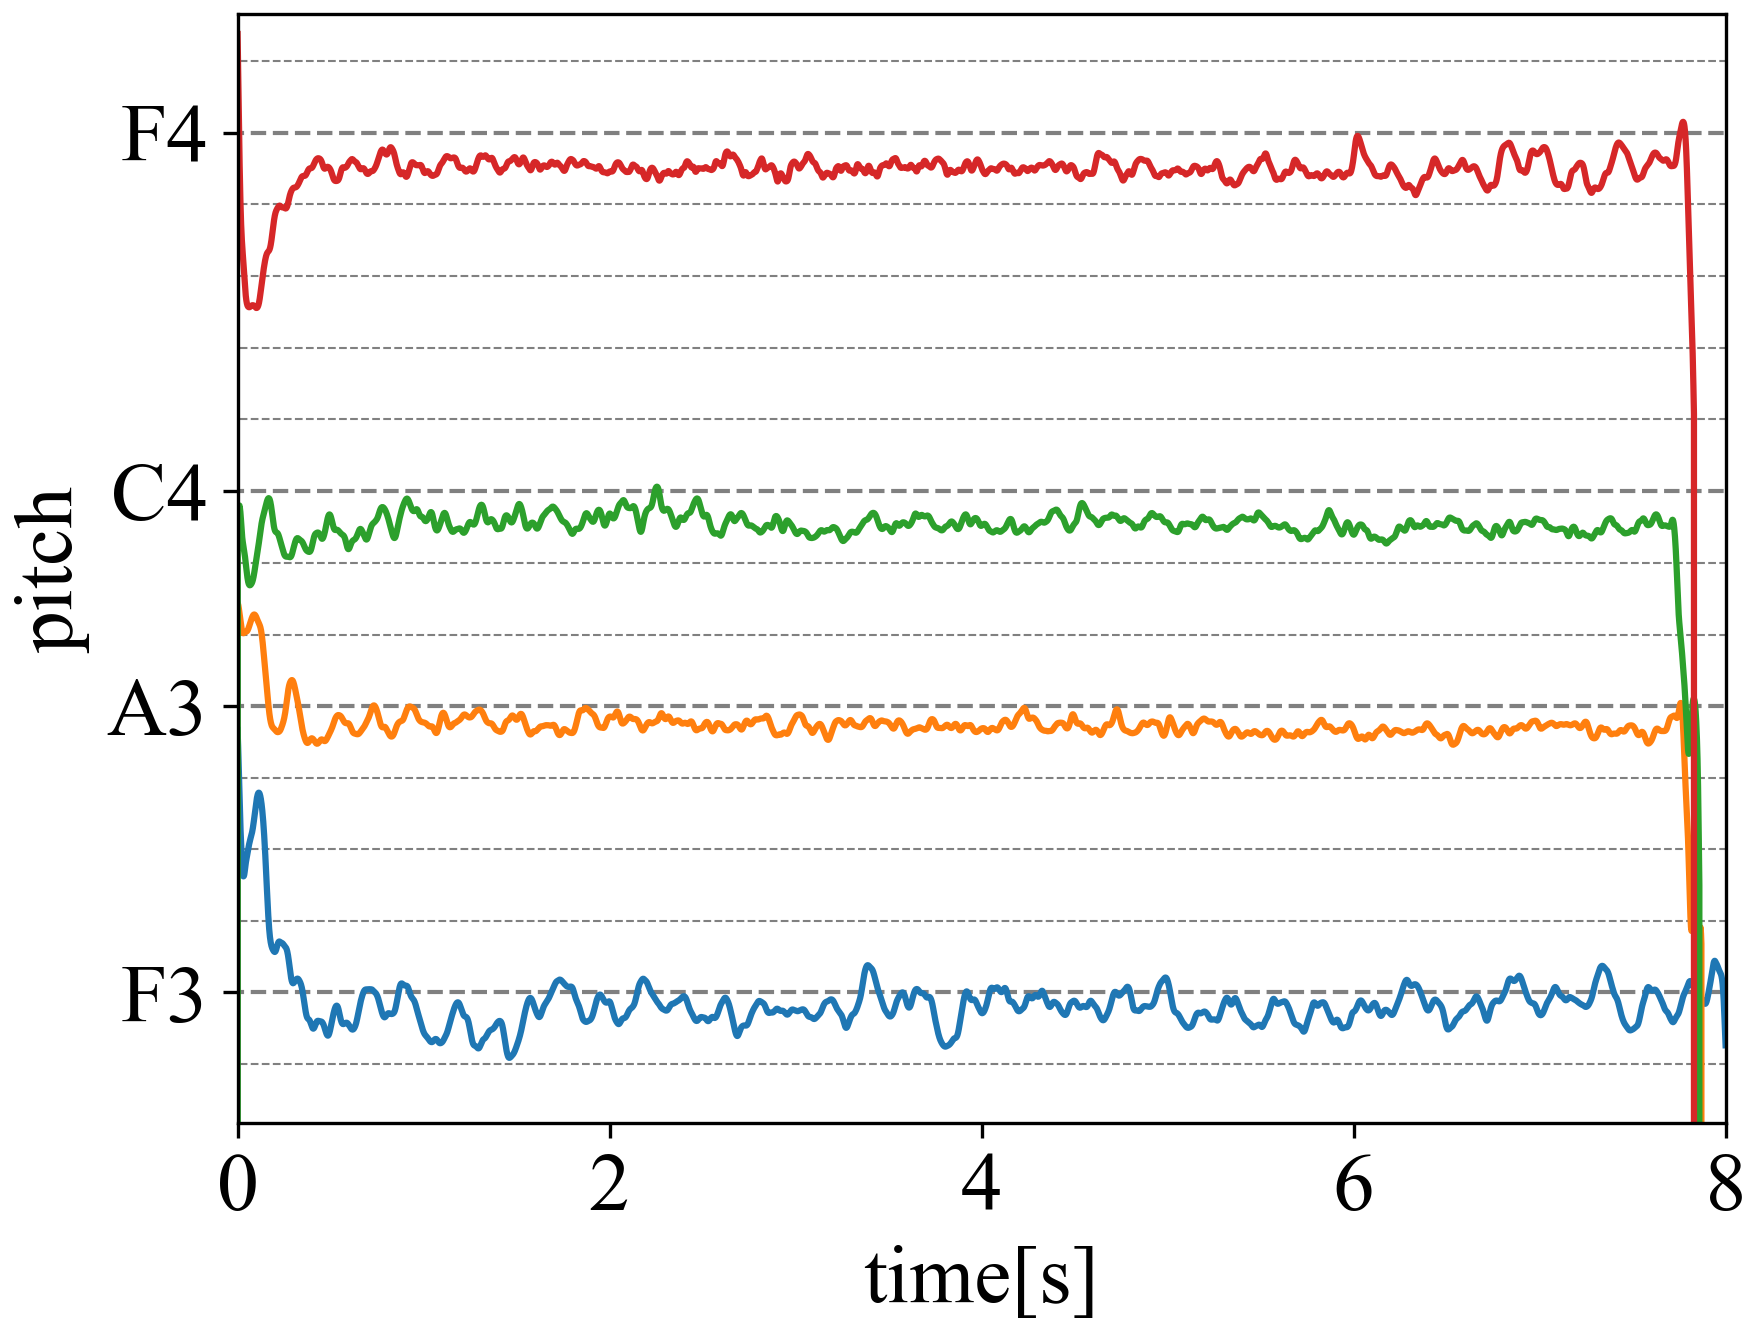
\includegraphics[width=5cm]{long/long_1_u.png} 
            \caption{被験者1の/u/単音発声}
            \label{lu}
        \end{center}
    \end{minipage}
\end{figure}

\begin{figure}[htbp]
    \begin{minipage}{0.33\hsize}
        \begin{center}
            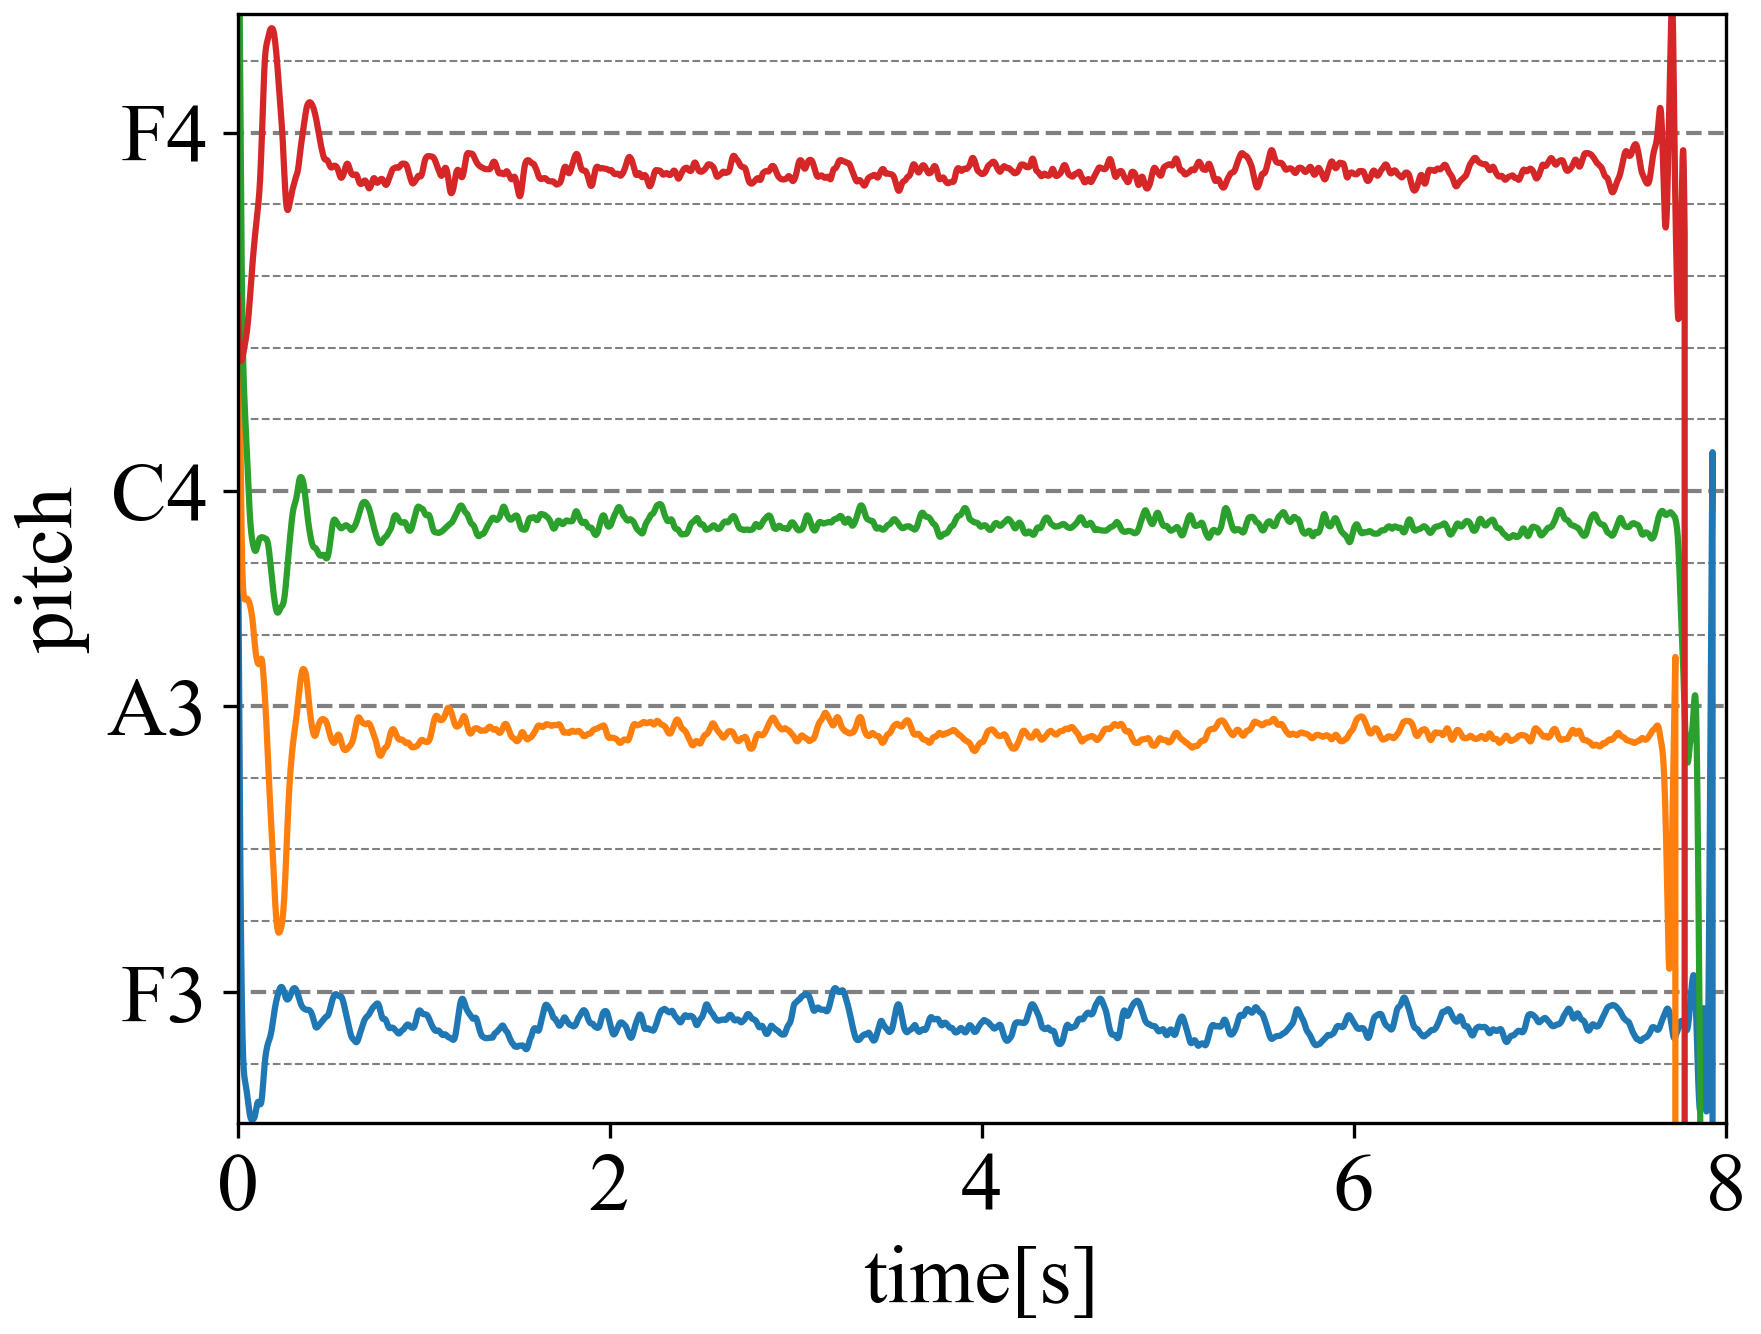
\includegraphics[width=5cm]{long/long_1_e.png}
            \caption{被験者1の/e/単音発声}
            \label{le}
        \end{center}
    \end{minipage}
    \begin{minipage}{0.33\hsize}
        \begin{center}
            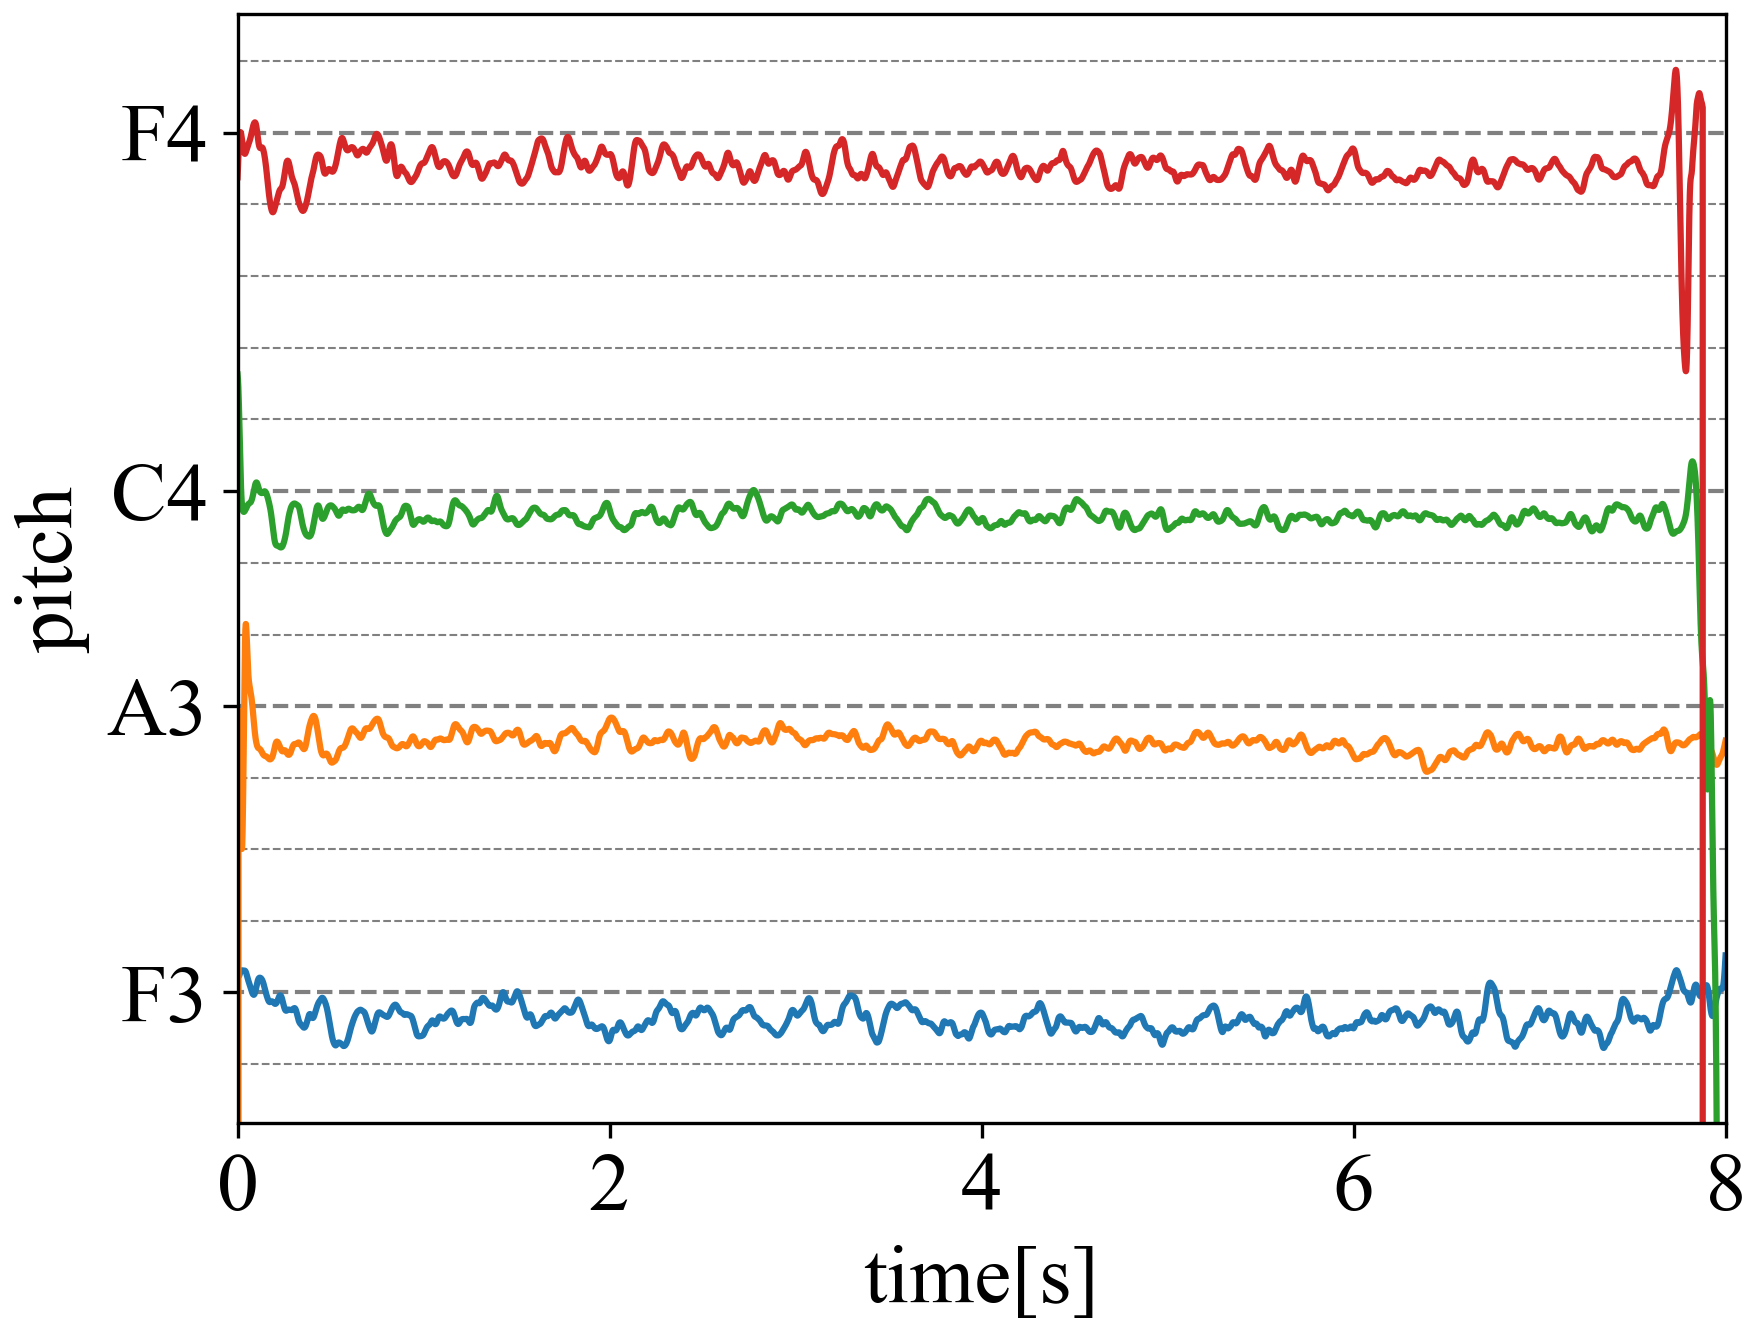
\includegraphics[width=5cm]{long/long_1_o.png}
            \caption{被験者1の/o/単音発声}
            \label{lo}
        \end{center}
    \end{minipage}
    \begin{minipage}{0.33\hsize} 
    \end{minipage}
    
\end{figure}

\subsection{上昇}
被験者1の上昇音形発声の$F_0$軌跡を図\ref{u1}に示す。左側が上昇前の母音、上側が上昇後の母音を表している。
上昇前が/i/のグラフにおいて上昇時に値が暴れているが、これは収録時に被験者が意図せず音を切り無音が発生したことに起因する。
一部の音声においてはオーバーシュートおよびプリパレーションの様子が見られる。

\begin{figure}[htbp]
    \begin{center}
      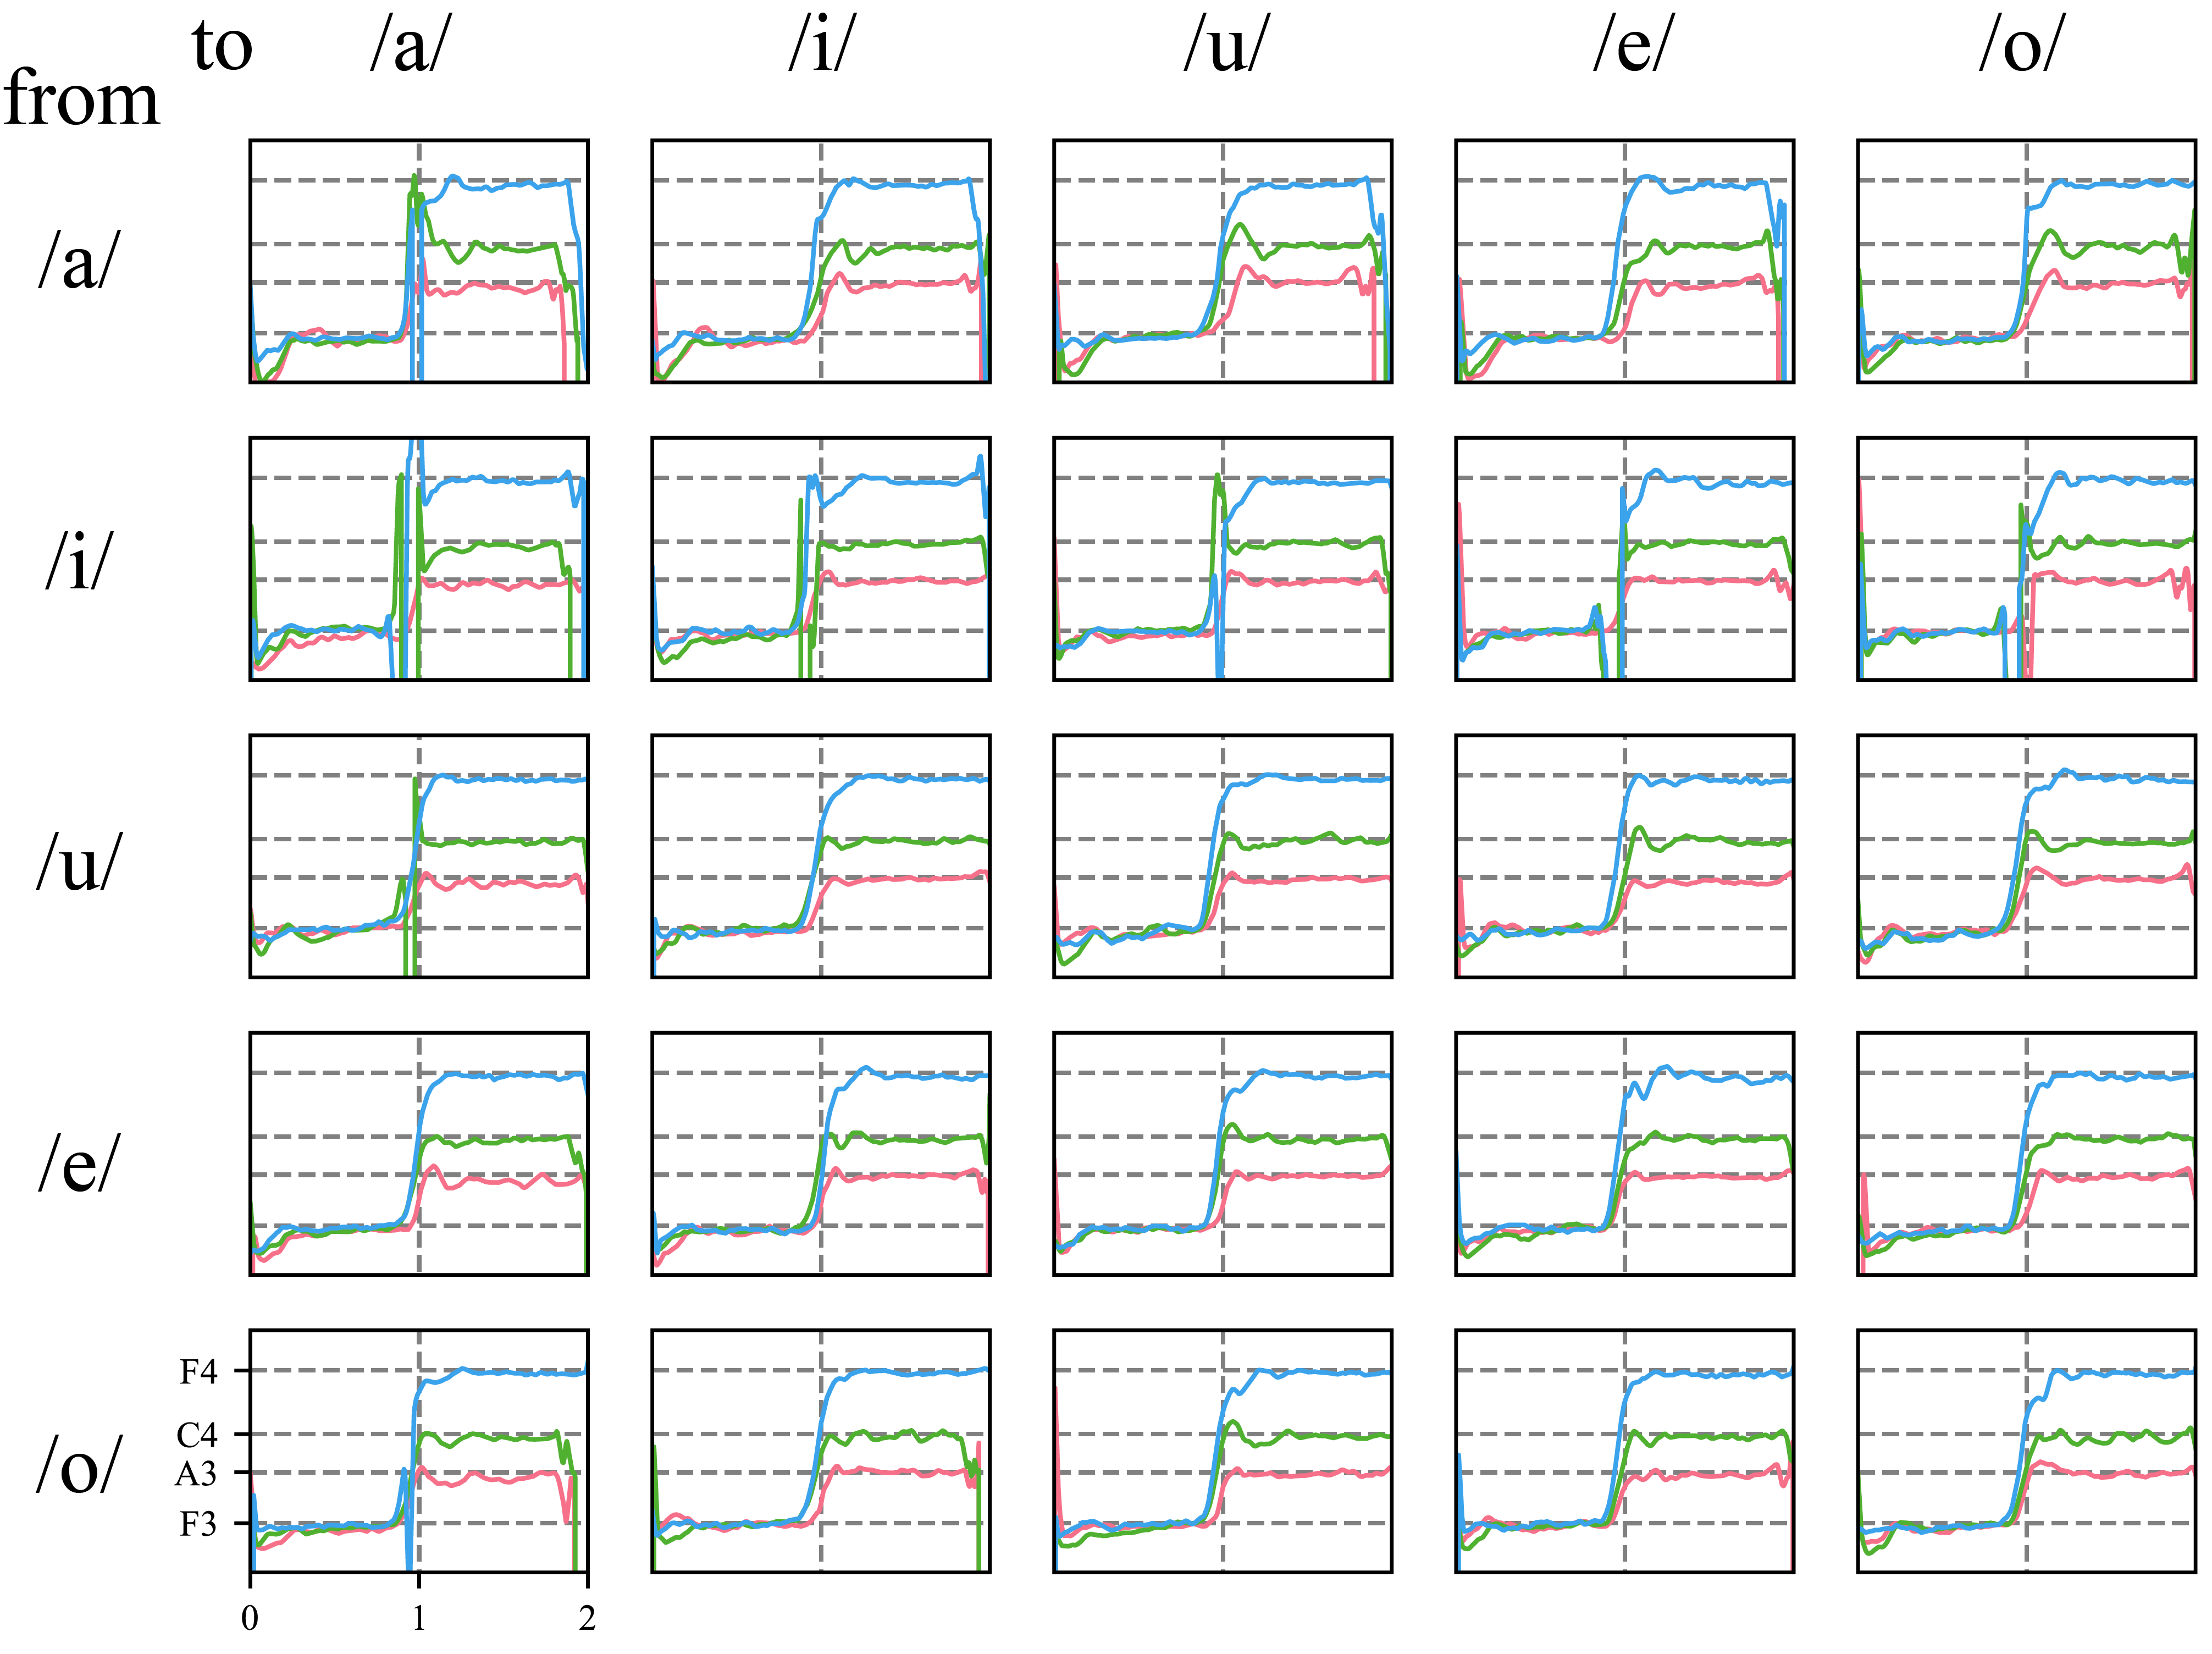
\includegraphics[clip,width=16.0cm]{up1.png}
      \caption{被験者1の上昇音形発声}
      \label{u1}
    \end{center}
\end{figure}

\subsection{下降}
被験者1の下降音形発声の$F_0$軌跡を図\ref{d1}に示す。こちらは上昇と比べると意図しない無音は発声しにくくなっている。
またプリパレーションはほとんど見られず、オーバーシュートが全体的に発生している。

\begin{figure}[htbp]
    \begin{center}
      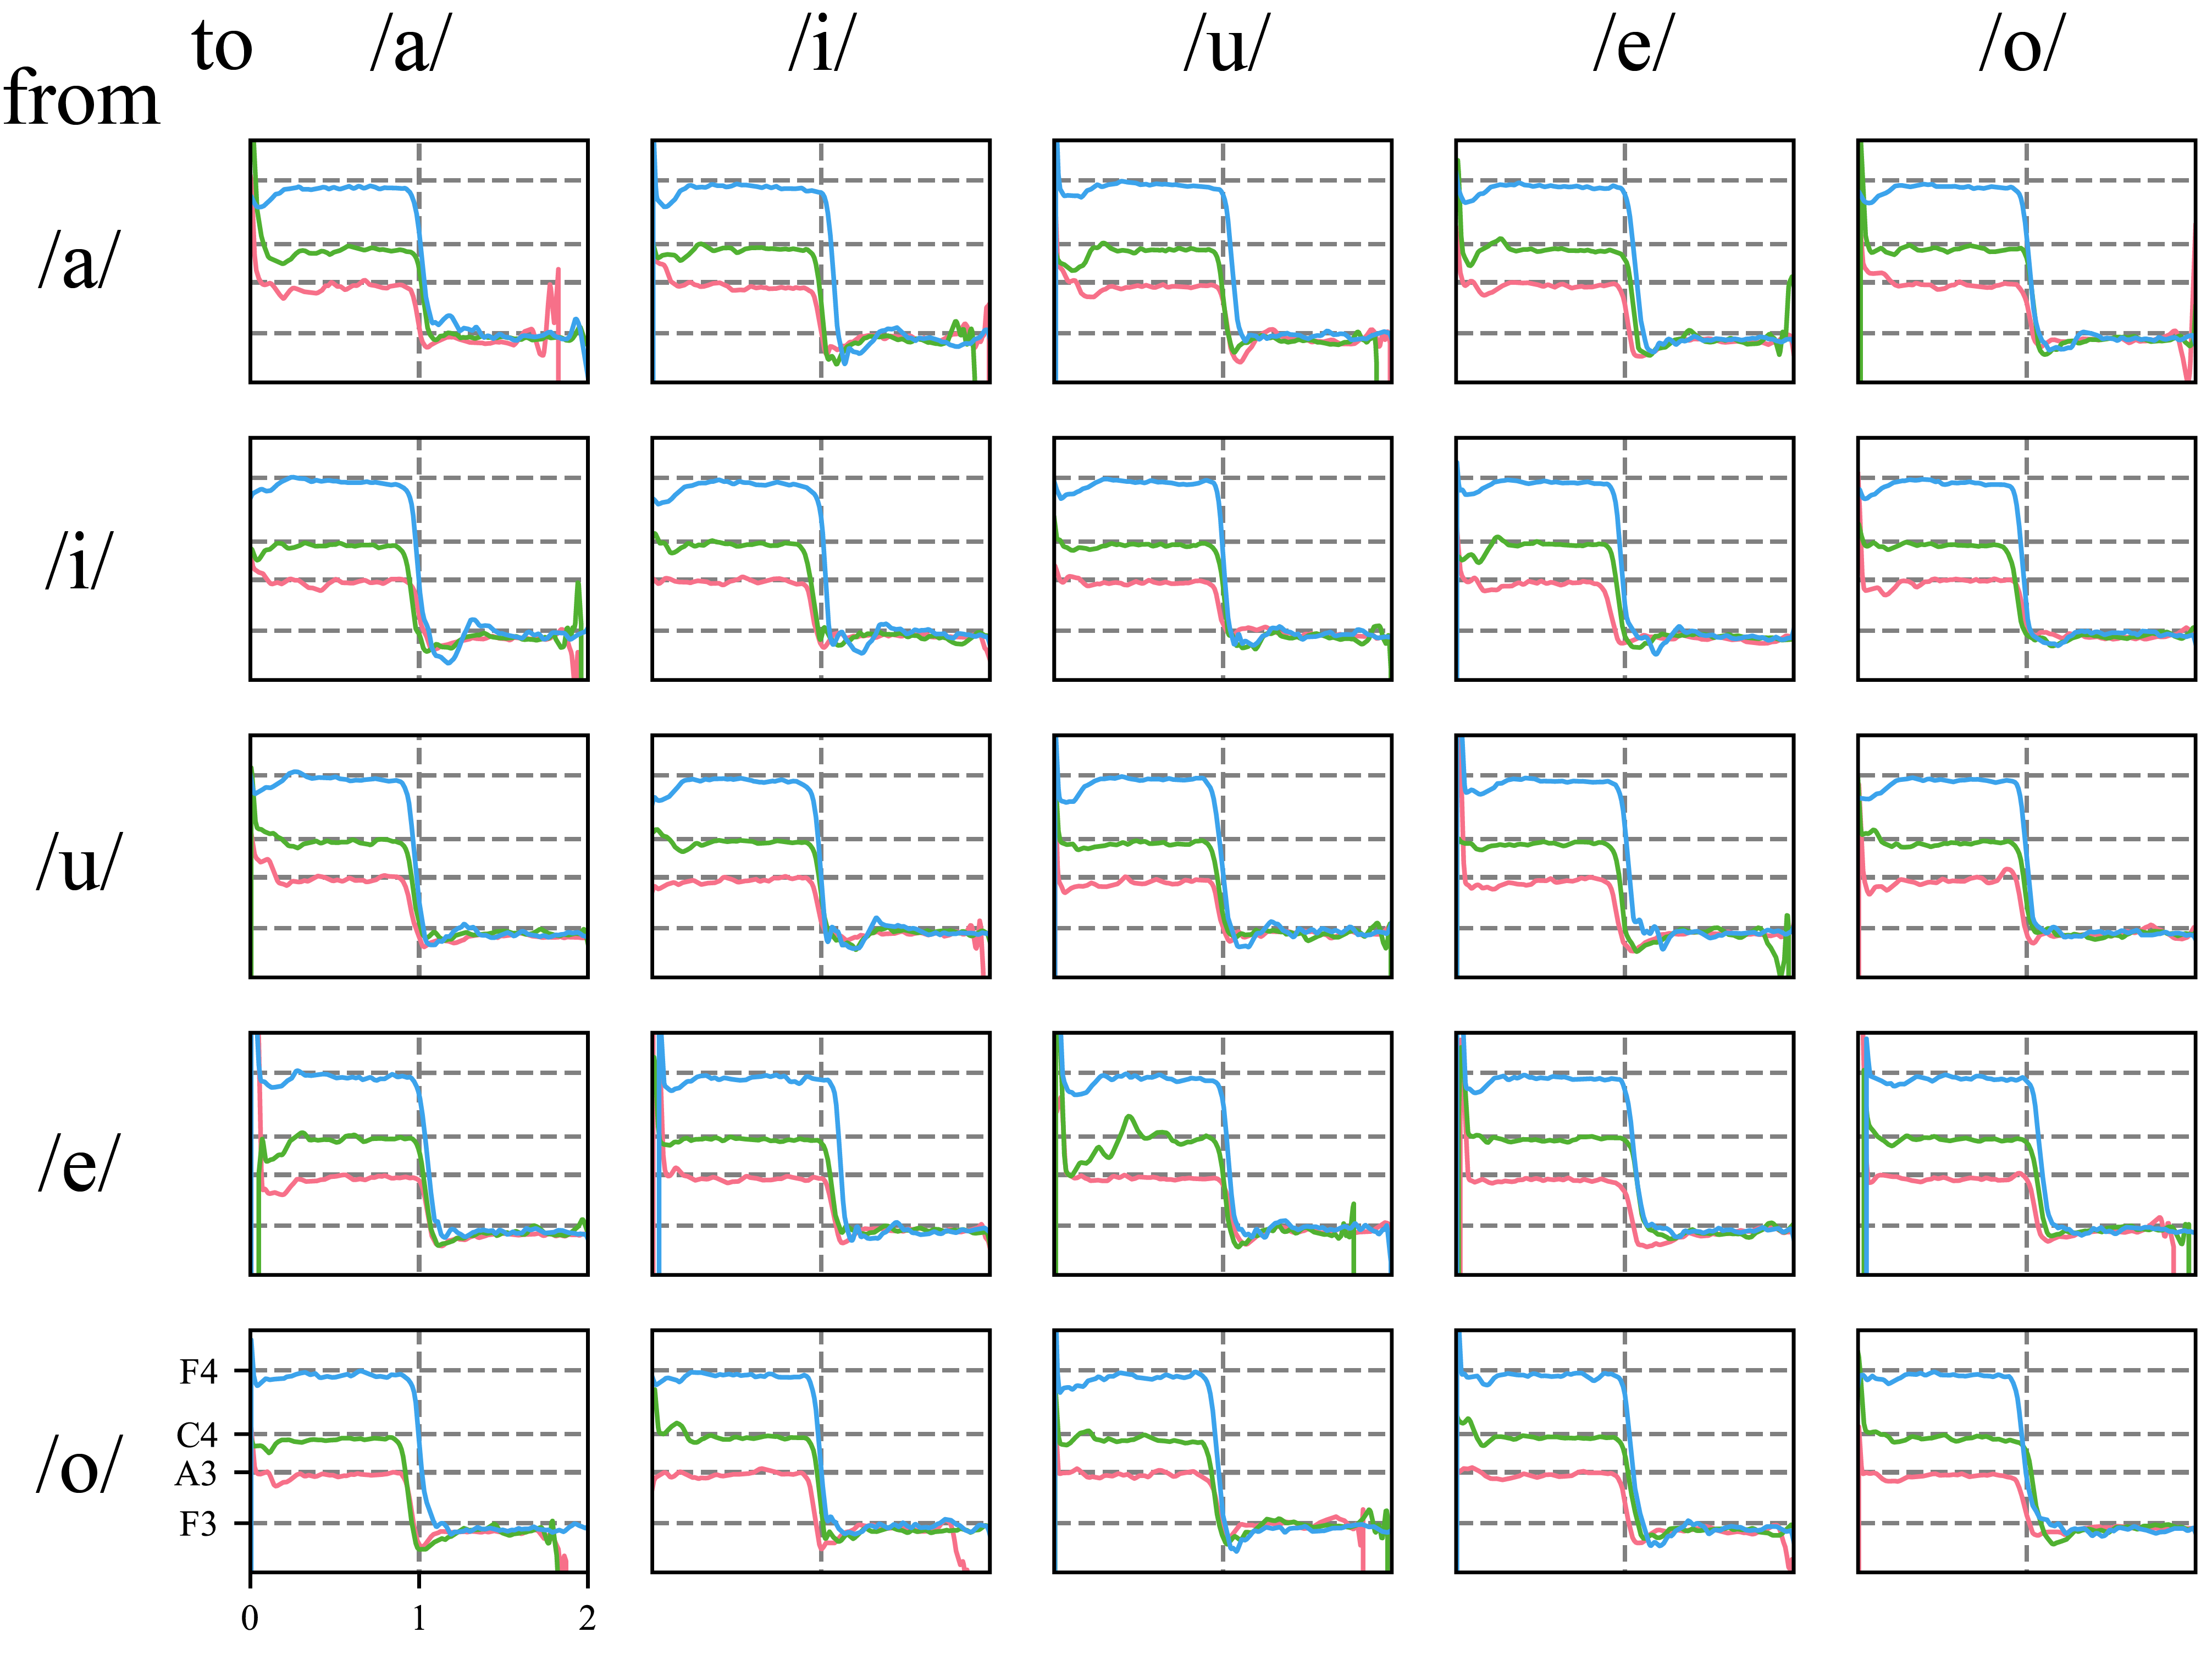
\includegraphics[clip,width=16.0cm]{down1.png}
      \caption{被験者1の下降音形発声}
      \label{d1}
    \end{center}
\end{figure}


%---------------------------%

\chapter{分析結果}
前項で得られたグラフだけでは、発声難度との関連性が見出せない。
そこで、前項のデータのうち特に単音発声の収録データとその発声難度の主観評価に着目して細かく分析を行い、
発声難度との関連性を検討する。

\section{主観評価との比較}
図\ref{difficulty}に、被験者による主観評価と平均音高のずれを示した。

\begin{figure}[htbp]
    \begin{center}
      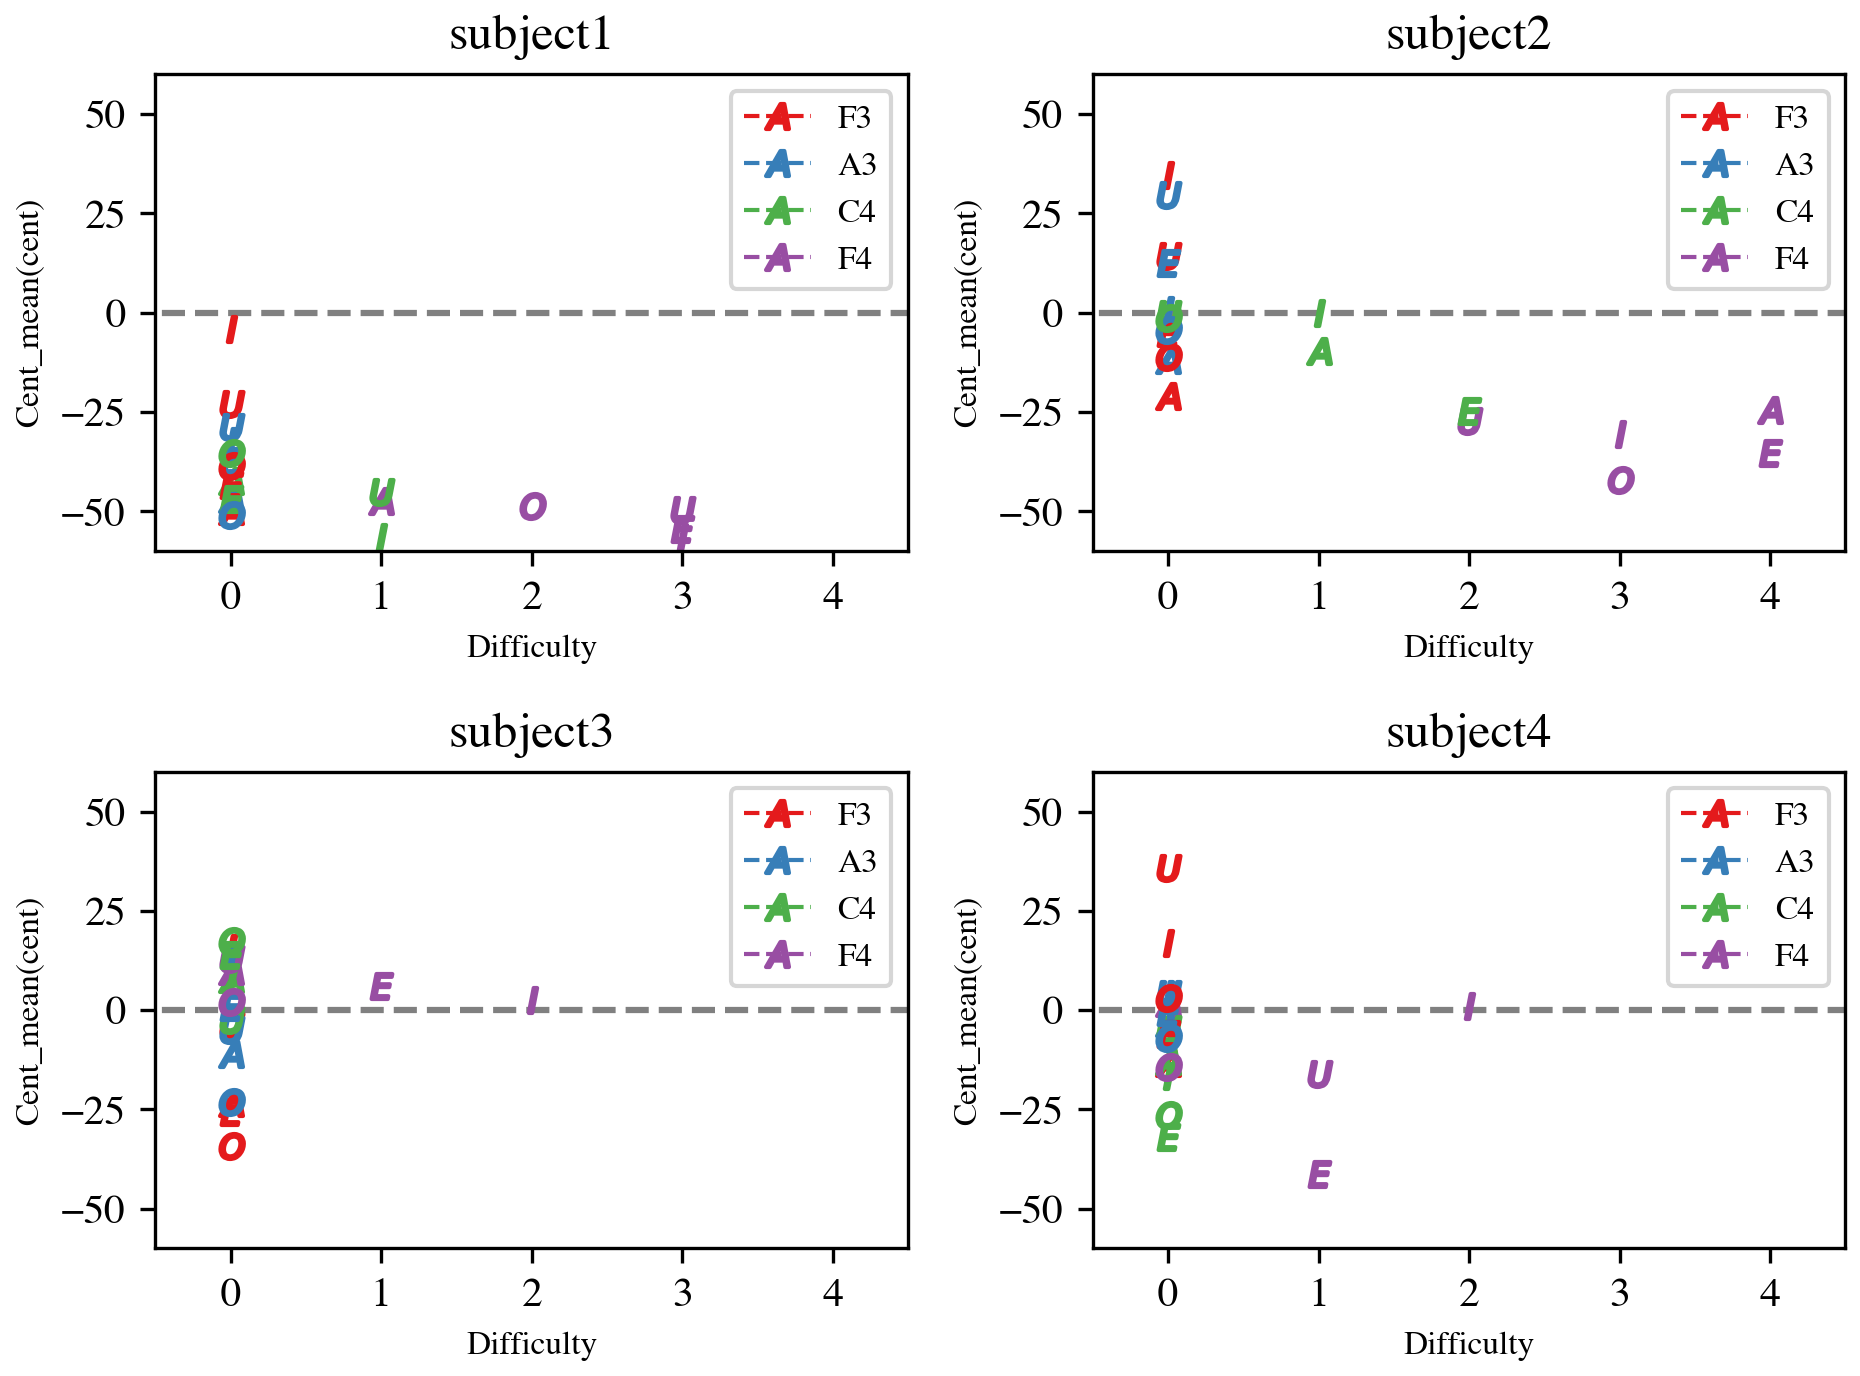
\includegraphics[clip,width=12.0cm]{ease.png}
      \caption{主観評価と$F_0$平均値の比較}
      \label{difficulty}
    \end{center}
\end{figure}

横軸は「発声しやすい」を0点、「どちらとも言えない」を1点、「発声しにくい」を2点としたときの2回の評価の和で、
数値が大きいほど発声しにくいことを表している。
縦軸は基準音高からのずれをセントで表している。
セントは音程を表す対数単位であり、12平均律においてオクターブを1200等分したものが1セントである。
すなわち100セントで1半音のずれを表す。

2つの音$x$と$y$の周波数が分かれば、その間のセント値は以下のように求められる。
\begin{equation}
    cent = 1200 \log_2 \frac{y}{x} 
\end{equation}

どの被験者においてもF4における/i/、/e/の母音で発声しにくいと評価しており、音高は正確なピッチから最大で50centほど低くなっている。
これは/i/、/u/の母音が狭め母音であるという構音上の性質が影響していると考えられる。
また、被験者1、2はC4においても発声しにくさを感じており、被験者3、4と比較して声区変換が早期に発生していると考えられる。




\section{単音発声の安定性}
単音発声は8秒間同じ音高を発声し続けるため、後半に音程の安定性が崩れることがあった。
この安定性を具体的に見るために、時間軸をいくつかの区間に分けて分析を行った。
歌い出し、歌い終わりの影響を避けるため、初めと終わりのそれぞれ1秒間を除いた6秒間を4つの区間に分け、
それぞれの区間において平均と標準偏差を求めた。
この結果を図\ref{long_mean_1}、\ref{long_mean_2}、\ref{long_mean_3}、\ref{long_mean_4}に示した。


\begin{figure}[htbp]
    \begin{minipage}{0.5\hsize}
        \begin{center}
            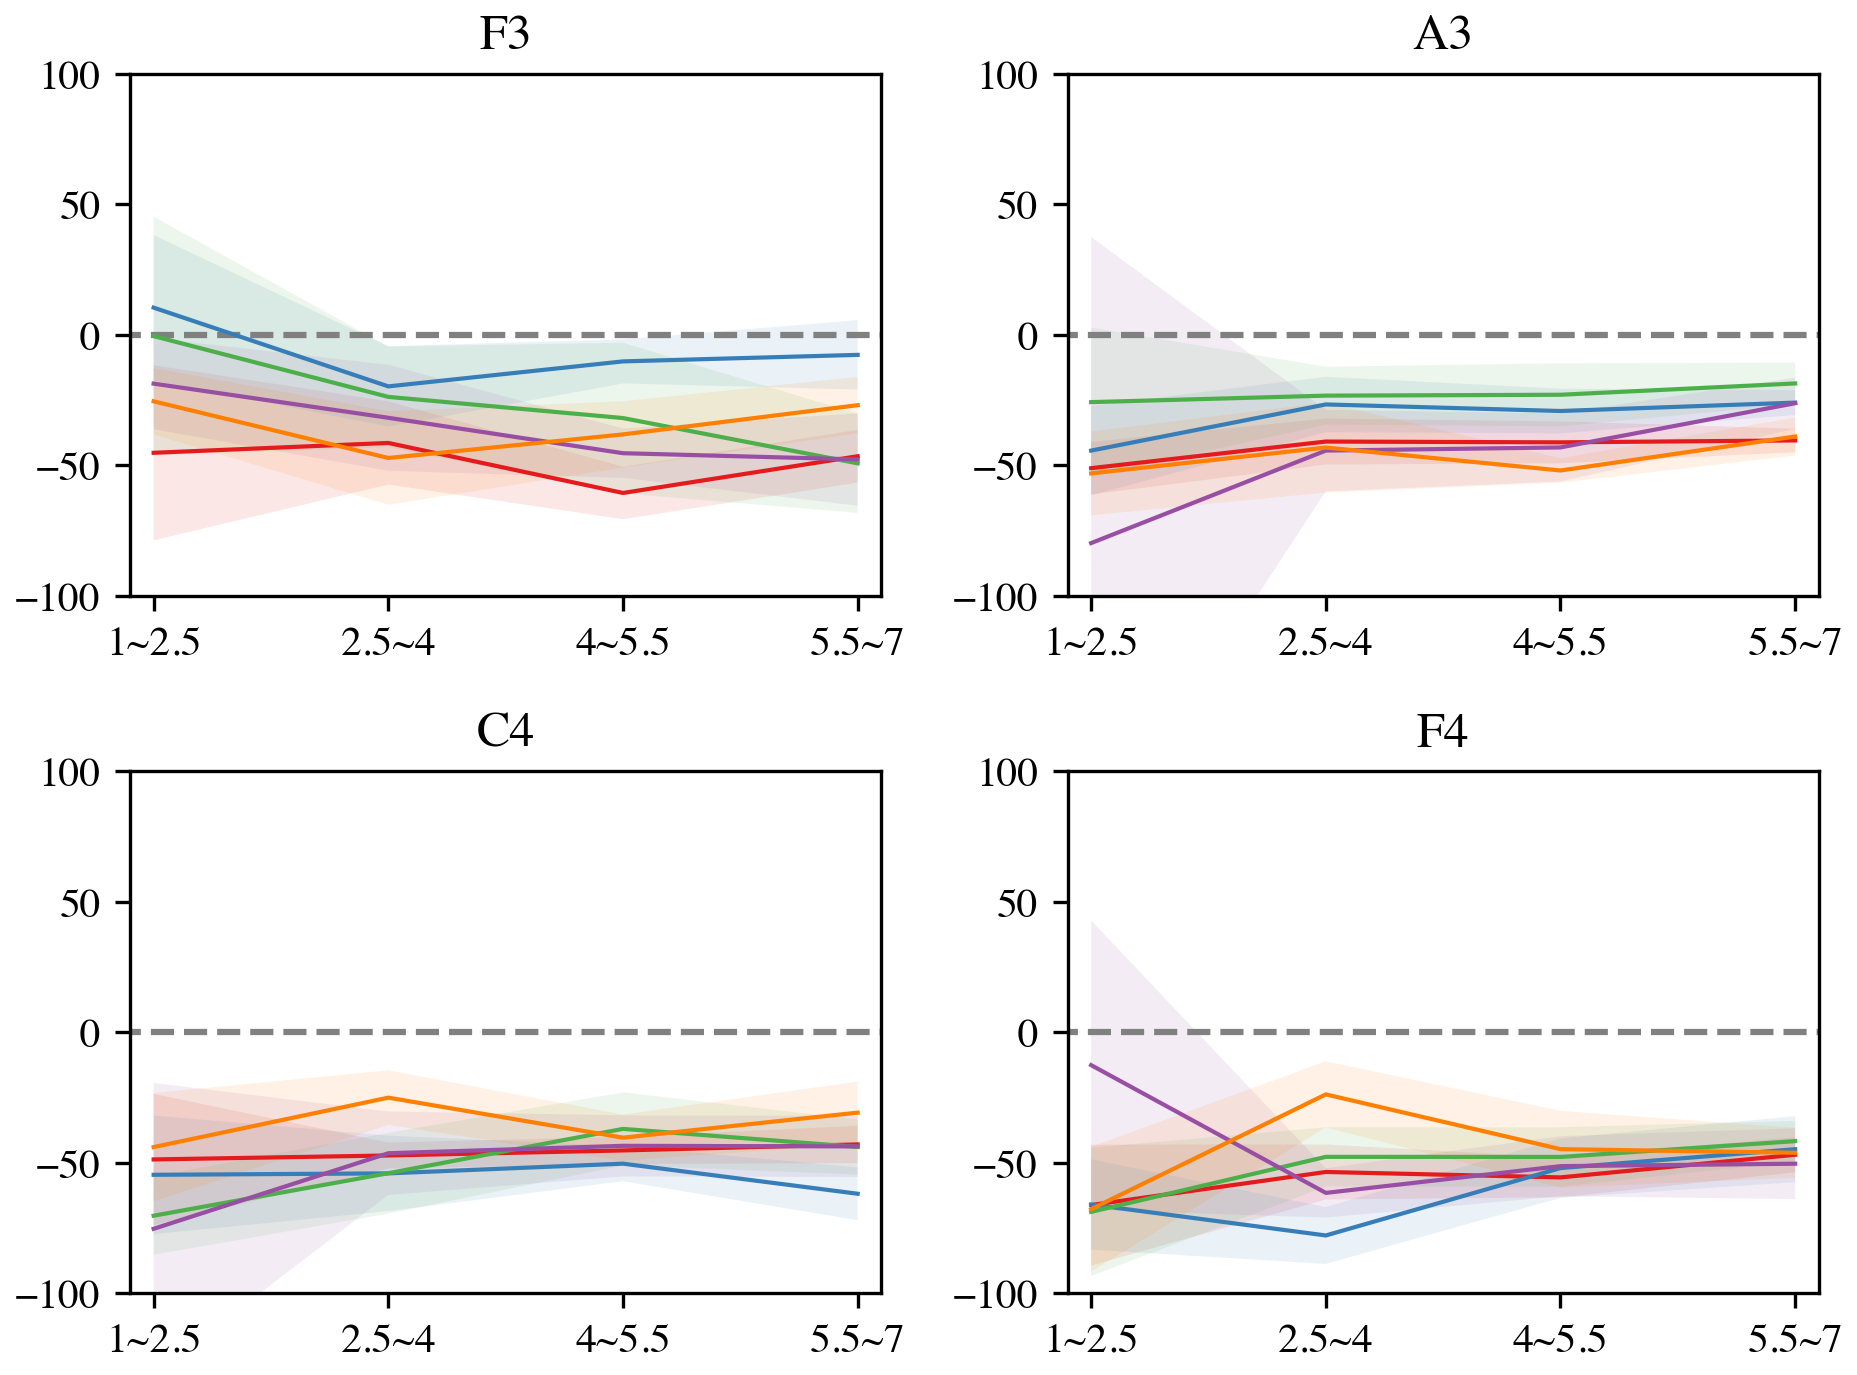
\includegraphics[clip,width=7.0cm]{long_mean_1.png}
          \end{center}
     \caption{被験者1の平均値変化}
     \label{long_mean_1}
    \end{minipage}
    \begin{minipage}{0.5\hsize}
        \begin{center}
            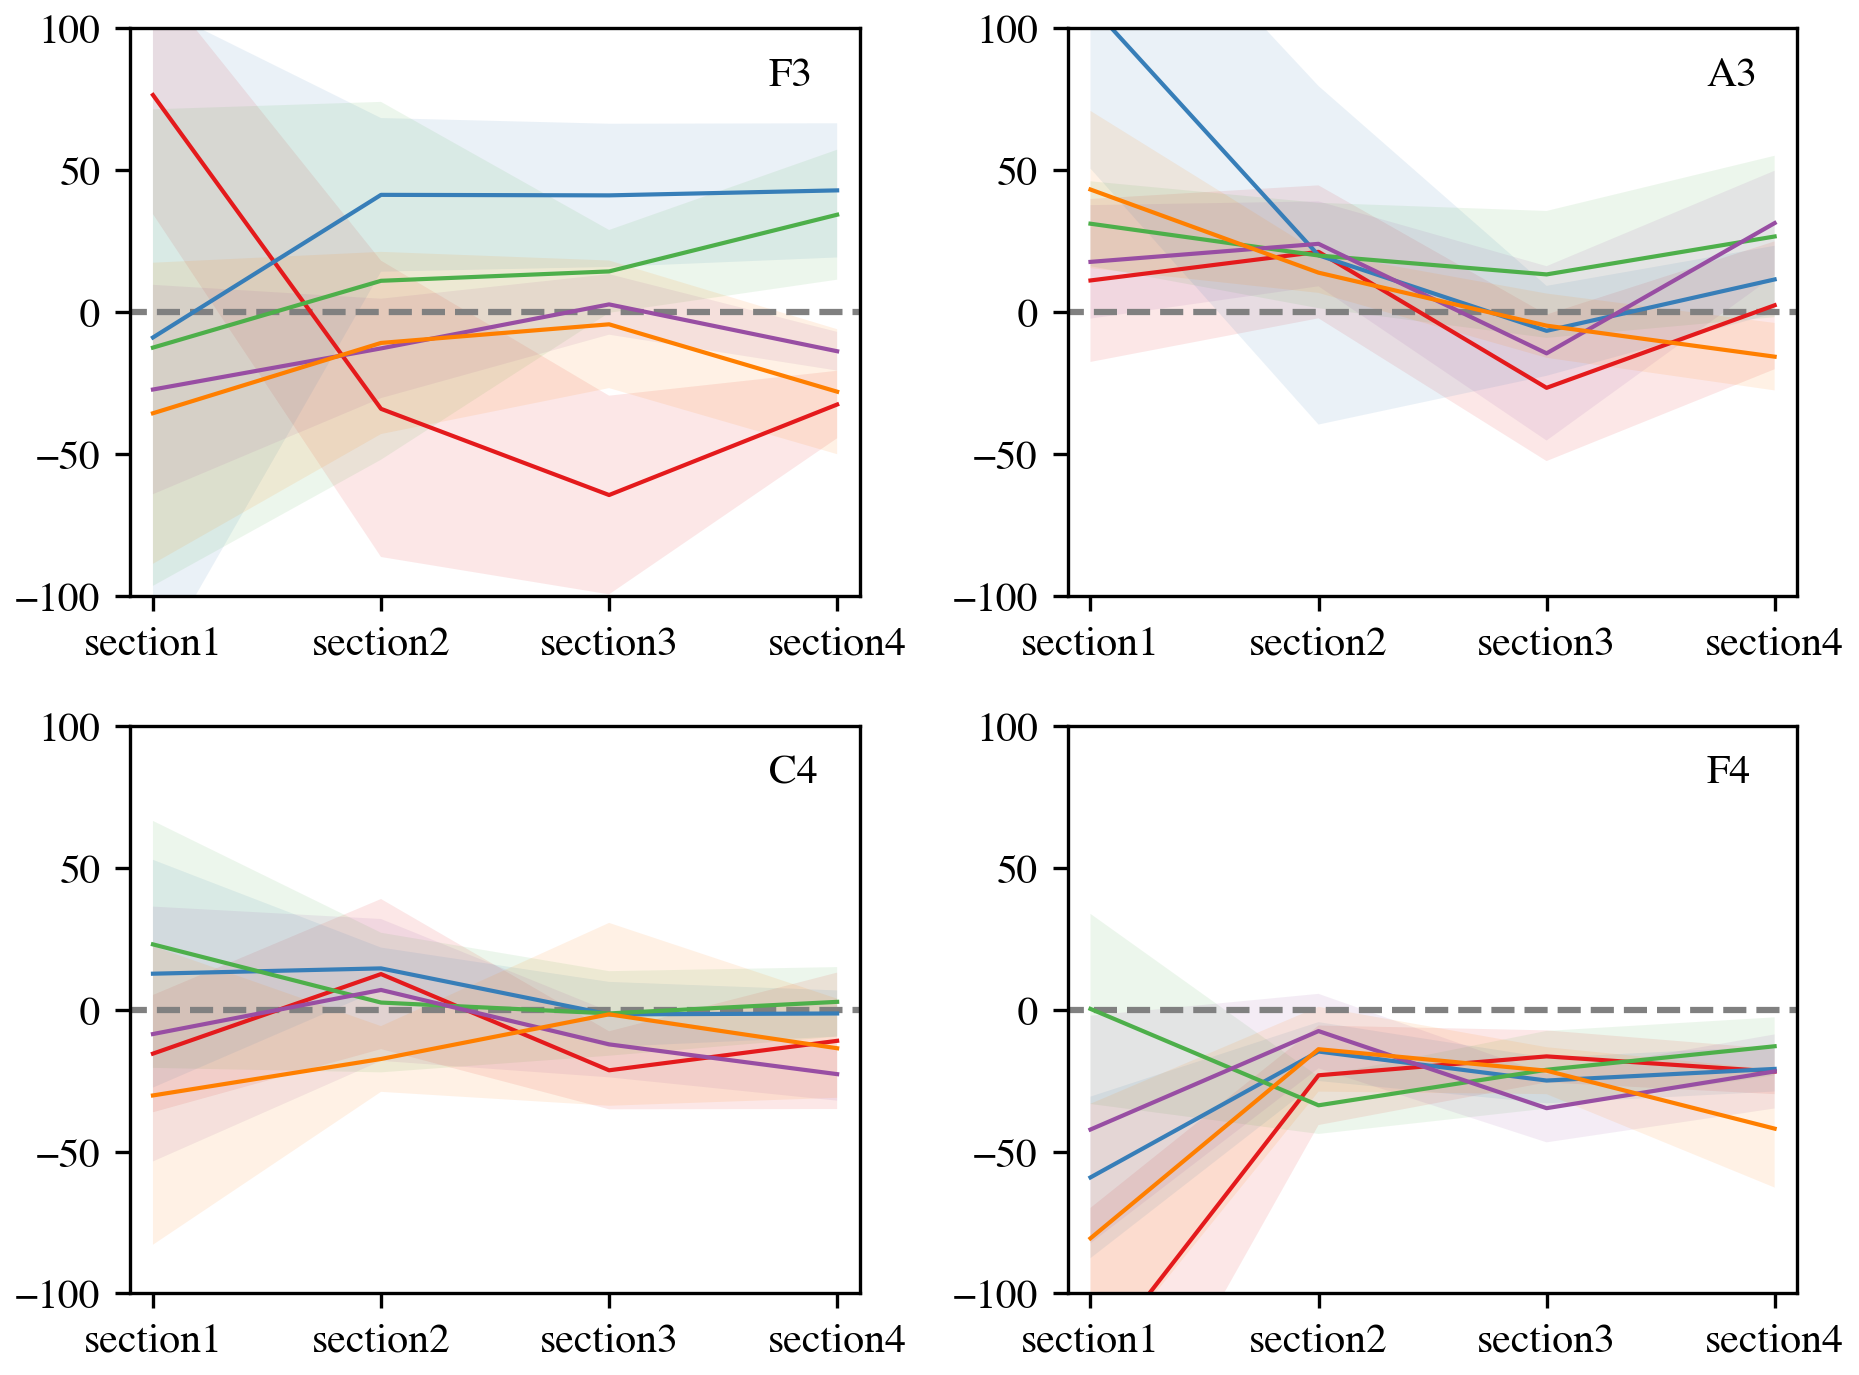
\includegraphics[clip,width=7.0cm]{long_mean_2.png}
          \end{center}
     \caption{被験者2の平均値変化}
     \label{long_mean_2}
    \end{minipage}
\end{figure}

\begin{figure}[htbp]
    \begin{minipage}{0.5\hsize}
        \begin{center}
            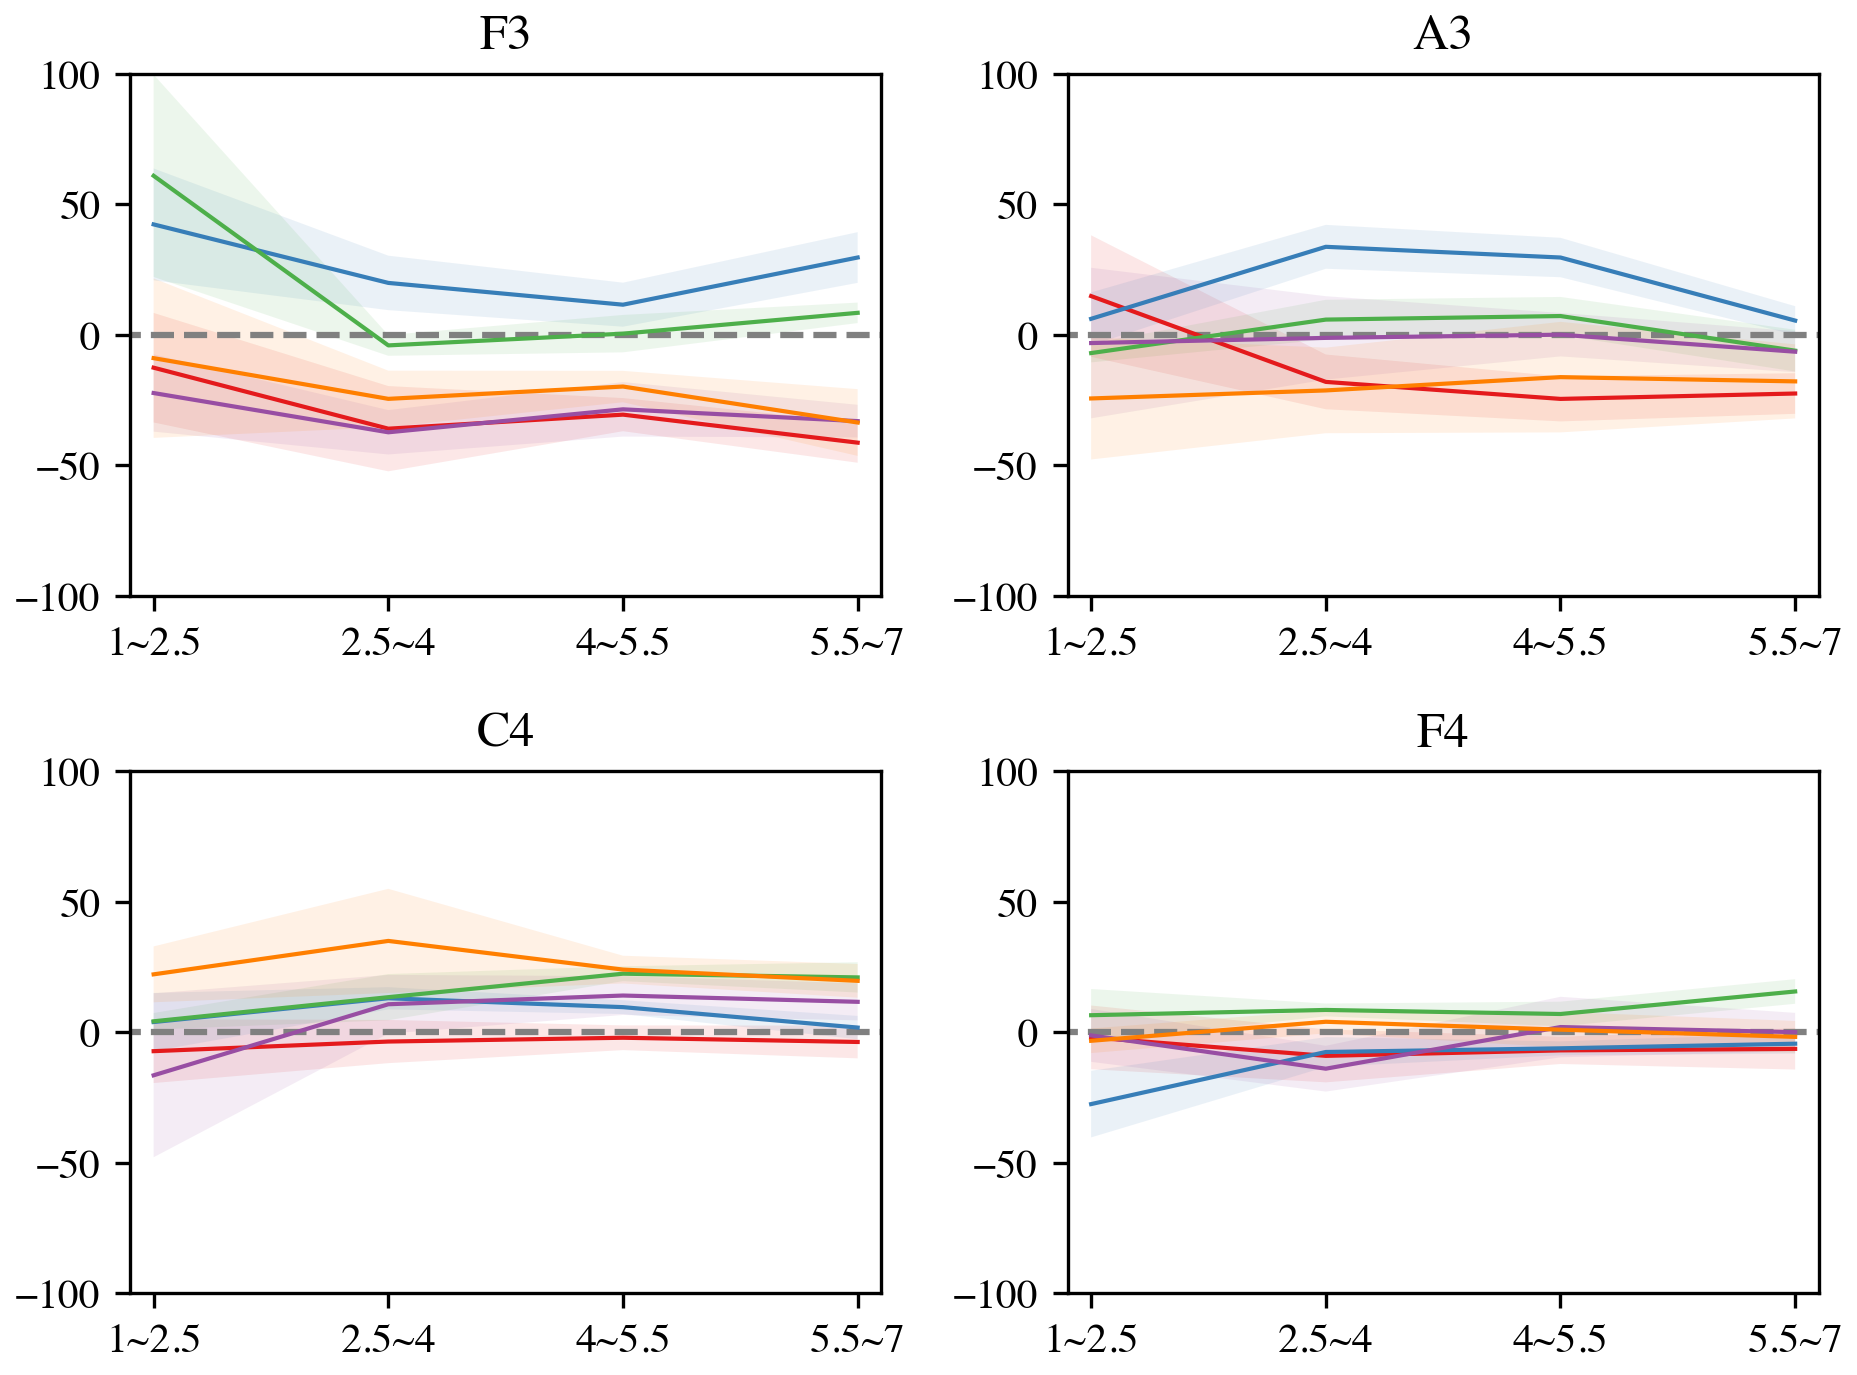
\includegraphics[clip,width=7.0cm]{long_mean_3.png}
          \end{center}
     \caption{被験者3の平均値変化}
     \label{long_mean_3}
    \end{minipage}
    \begin{minipage}{0.5\hsize}
        \begin{center}
            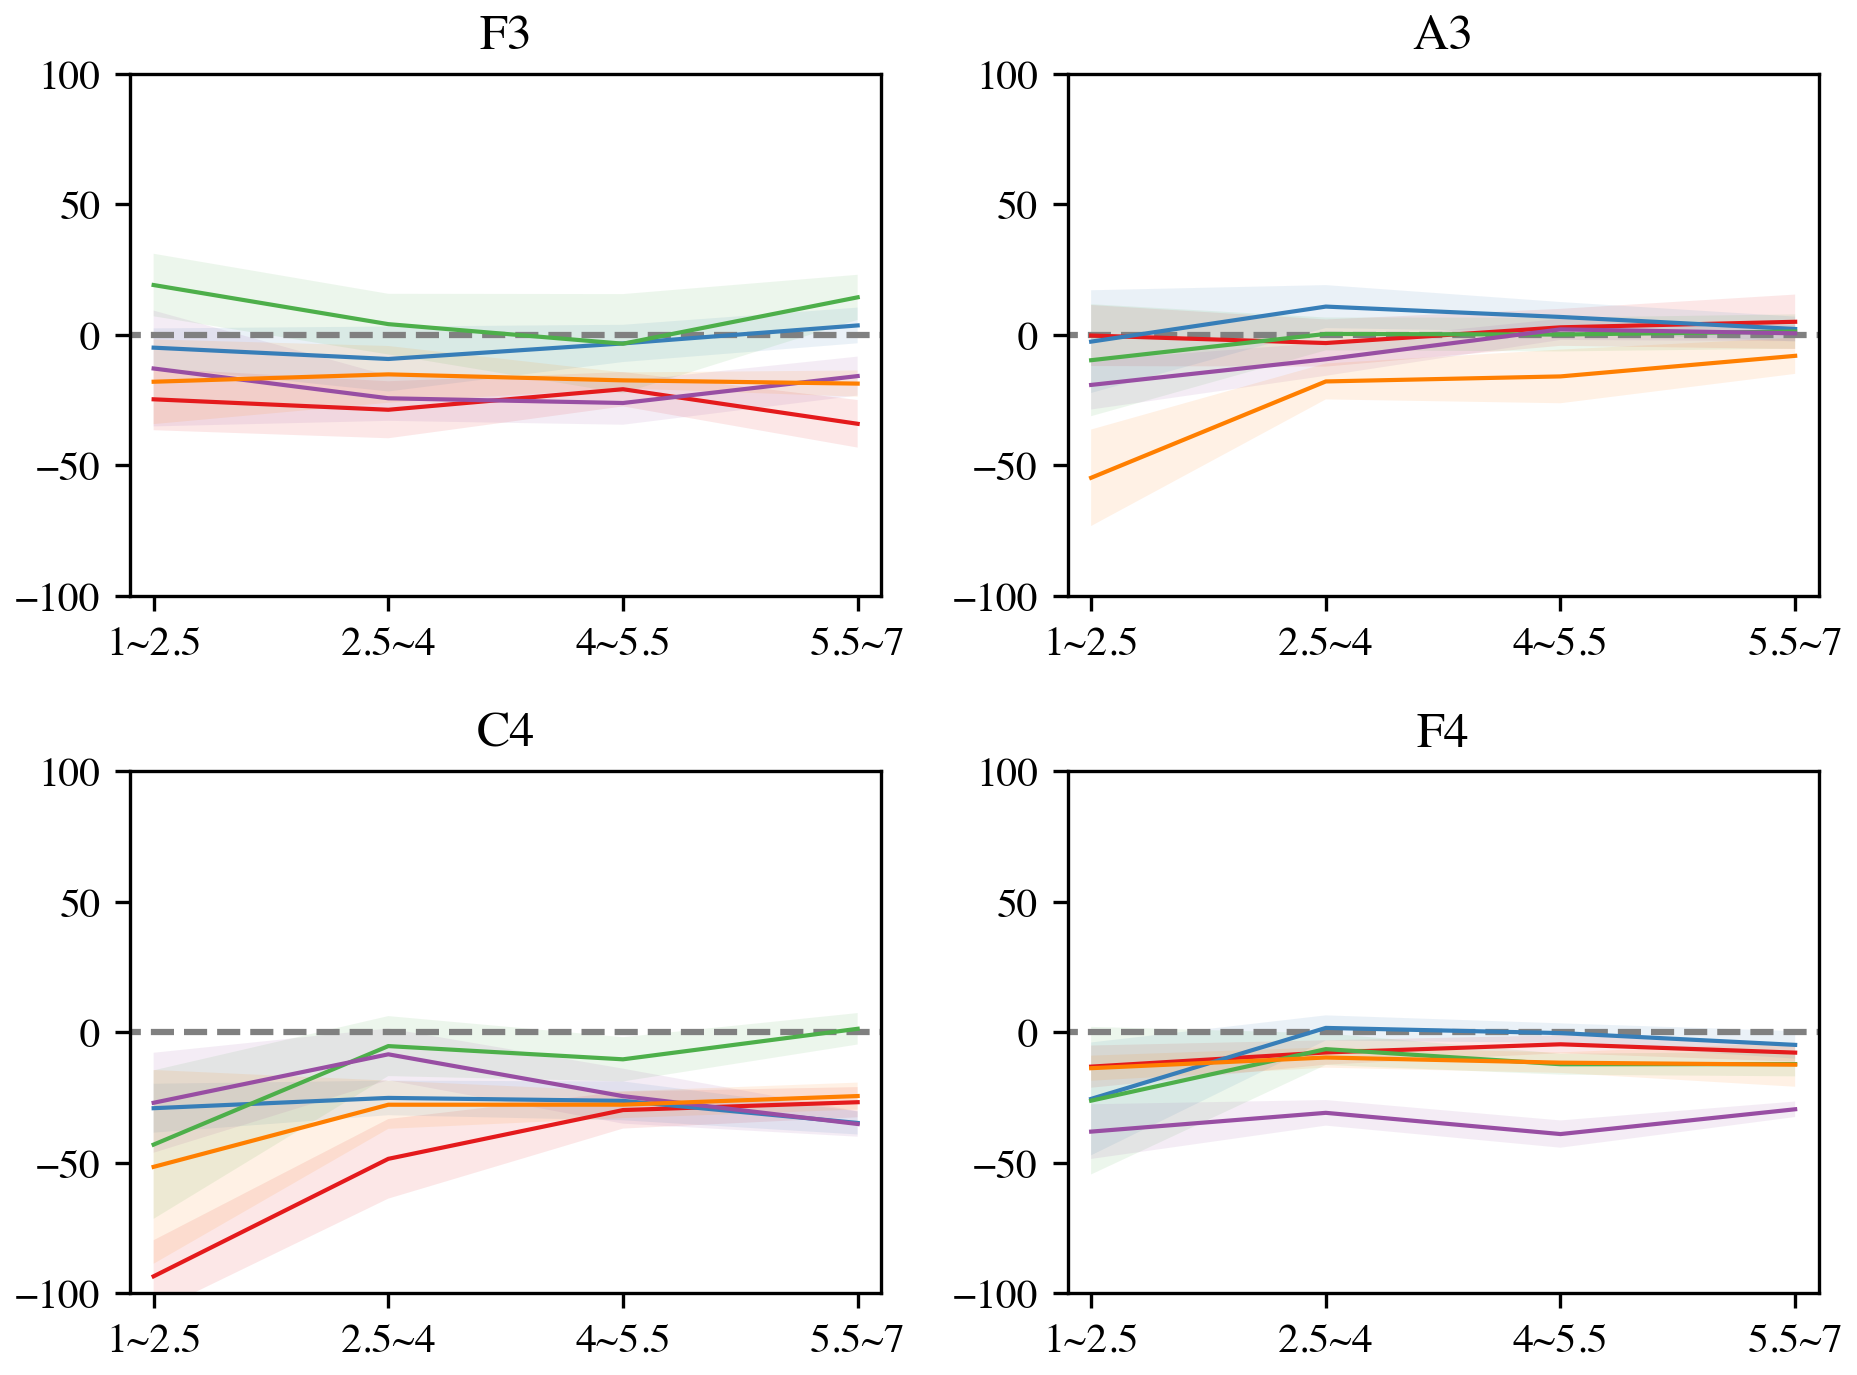
\includegraphics[clip,width=7.0cm]{long_mean_4.png}
          \end{center}
     \caption{被験者4の平均値変化}
     \label{long_mean_4}
    \end{minipage}
\end{figure}

これらを見ると、音高が上がるほど最終的な音のぶれが小さくなっていることがわかる。
このことから、音高を合わせ続けることについては発声時の感覚に反し低音の方が難しいと考えられる。
また、F3において/i/、/u/の音高の平均が他の母音に比べて全体的に高くなっており、
低音域では/i/、/u/発声時における歌唱者の知覚する音高が他の母音と比べて相対的に高くなっていることを示唆している。
これは/i/、/u/の$F_1$が発声している音高と近いことが原因の一つと考えられる。

被験者1は音高の目標点が基準より全体的に低めであり、被験者の想定する正しい音高と実際の音高が異なる可能性がある。
被験者2は高音でも標準偏差が大きいままであり、地声の音域外の音高を無理に発声しようとした結果不安定になったと考えられる。
また被験者3、4は被験者1、2と比べると標準偏差が全体的に小さい。
このように、被験者ごとに個人の特性が強く出ていると考えられる。



\section{$F_0$の周波数変調}
続いて、発声の不安定性がヴィブラートのように$F_0$に現れている可能性から$F_0$動的変動成分に着目する。
歌い出しと歌い終わりを除く6秒間の$F_0$軌跡を波形としてフーリエ変換を行い、どのような成分が含まれるかを確かめた。
詳細な条件は表\ref{table:F0Moduration}の通りである。


\begin{table}[h]
    \caption{フーリエ変換の詳細}
    \label{table:F0Moduration}
    \centering
    \begin{tabular}{clll}
        \hline
        データ長 & 6001点\\
        フレームレート & 1000Hz\\
        窓長 & 500点\\
        シフト長 & 50点\\
        \hline
    \end{tabular}
\end{table}


なお、窓長で切り出したデータに対して、平均が0になるように値を移動してからハミング窓をかけた。得られたモジュレーションの全体平均をとったものが
図\ref{long_spectrogram_1}、\ref{long_spectrogram_2}、
\ref{long_spectrogram_3}、\ref{long_spectrogram_4}である。



被験者3と4、特に被験者4に強く見られる現象として、/i/、/u/の狭め母音に対して80Hz周辺でピークが生じている。
この原因の一つとして、音源-フィルタ相互作用の影響が考えられる。
/i/、/u/の$F_1$は300Hz前後であり発声している音高F3(174.6Hz)と比較的近いことから、
声帯音源の発声機構と声道の間に強い干渉が生じ\cite{source-filterCoupling}、音源-フィルタ相互作用によって基本周波数に変化が生じたと考えられる。\cite{tsuburagi}

\begin{figure}[htbp]
    \begin{center}
      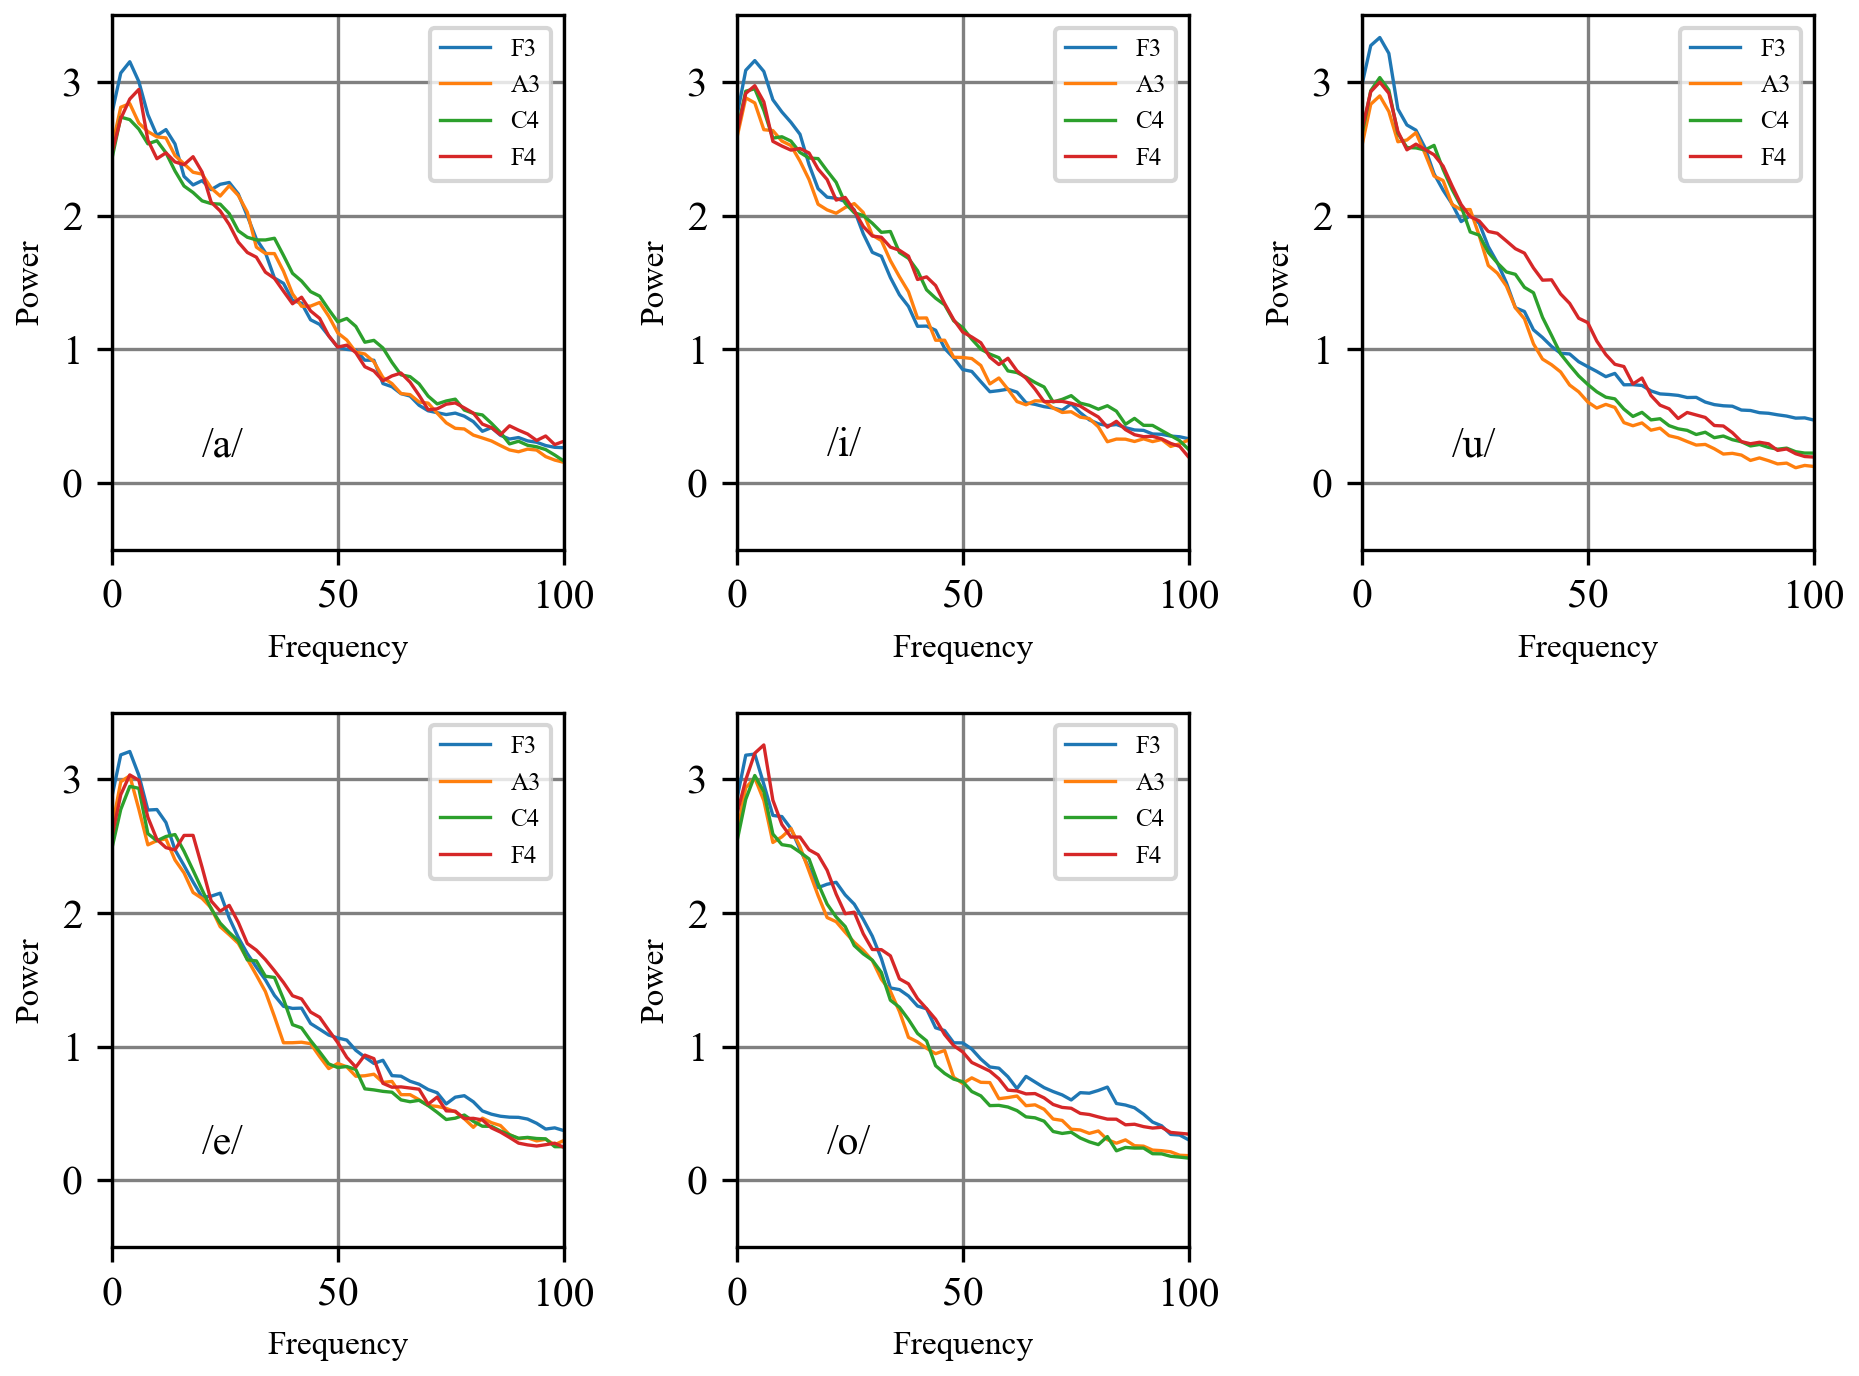
\includegraphics[clip,width=12.0cm]{long_spectrogram_1.png}
      \caption{被験者1のモジュレーションの全体平均}
      \label{long_spectrogram_1}
    \end{center}
\end{figure}

\begin{figure}[htbp]
    \begin{center}
      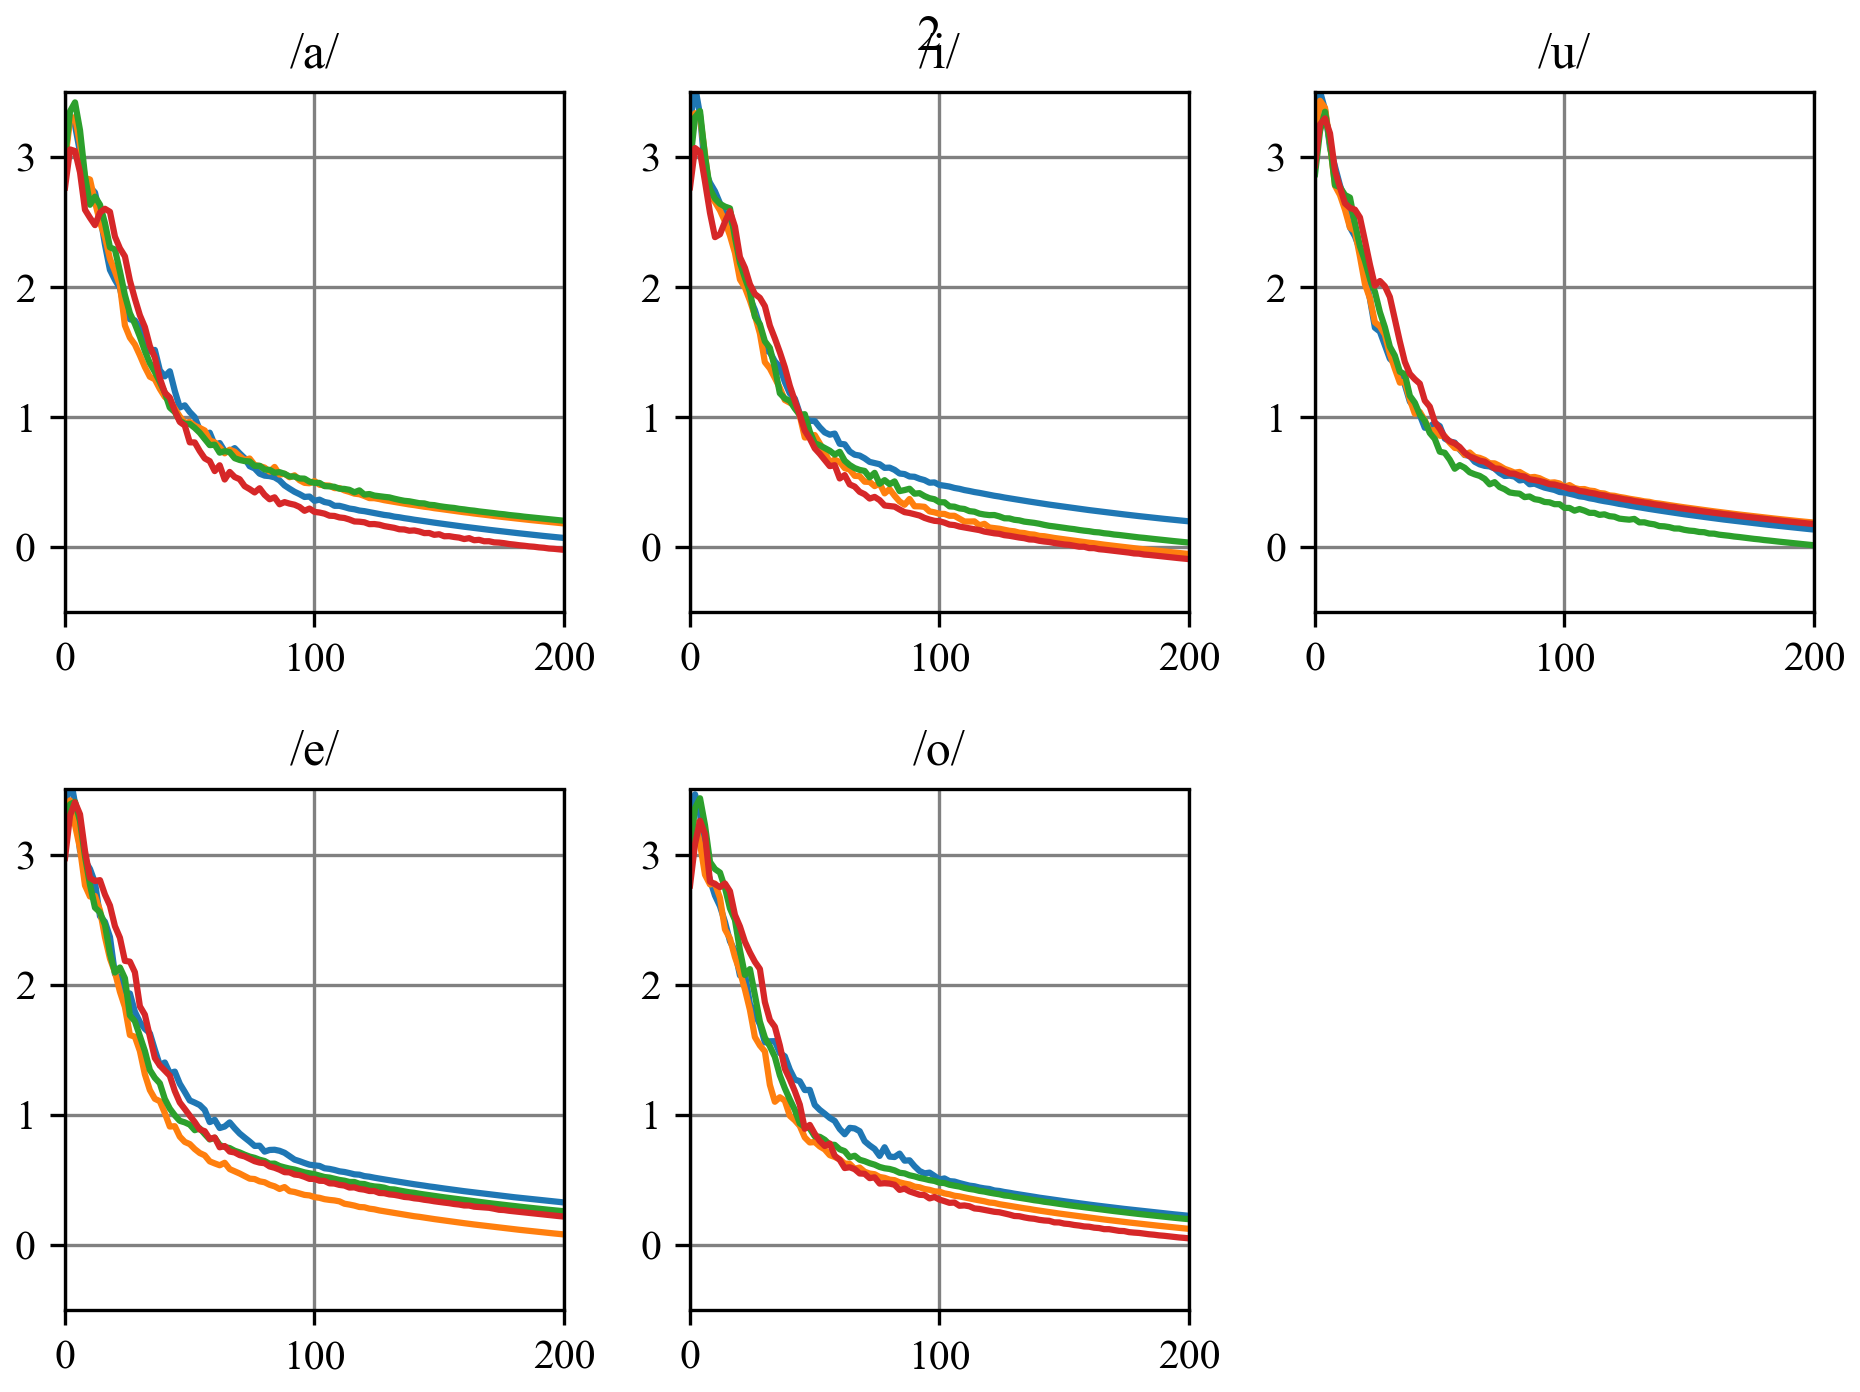
\includegraphics[clip,width=12.0cm]{long_spectrogram_2.png}
      \caption{被験者2のモジュレーションの全体平均}
      \label{long_spectrogram_2}
    \end{center}
\end{figure}

\begin{figure}[htbp]
    \begin{center}
      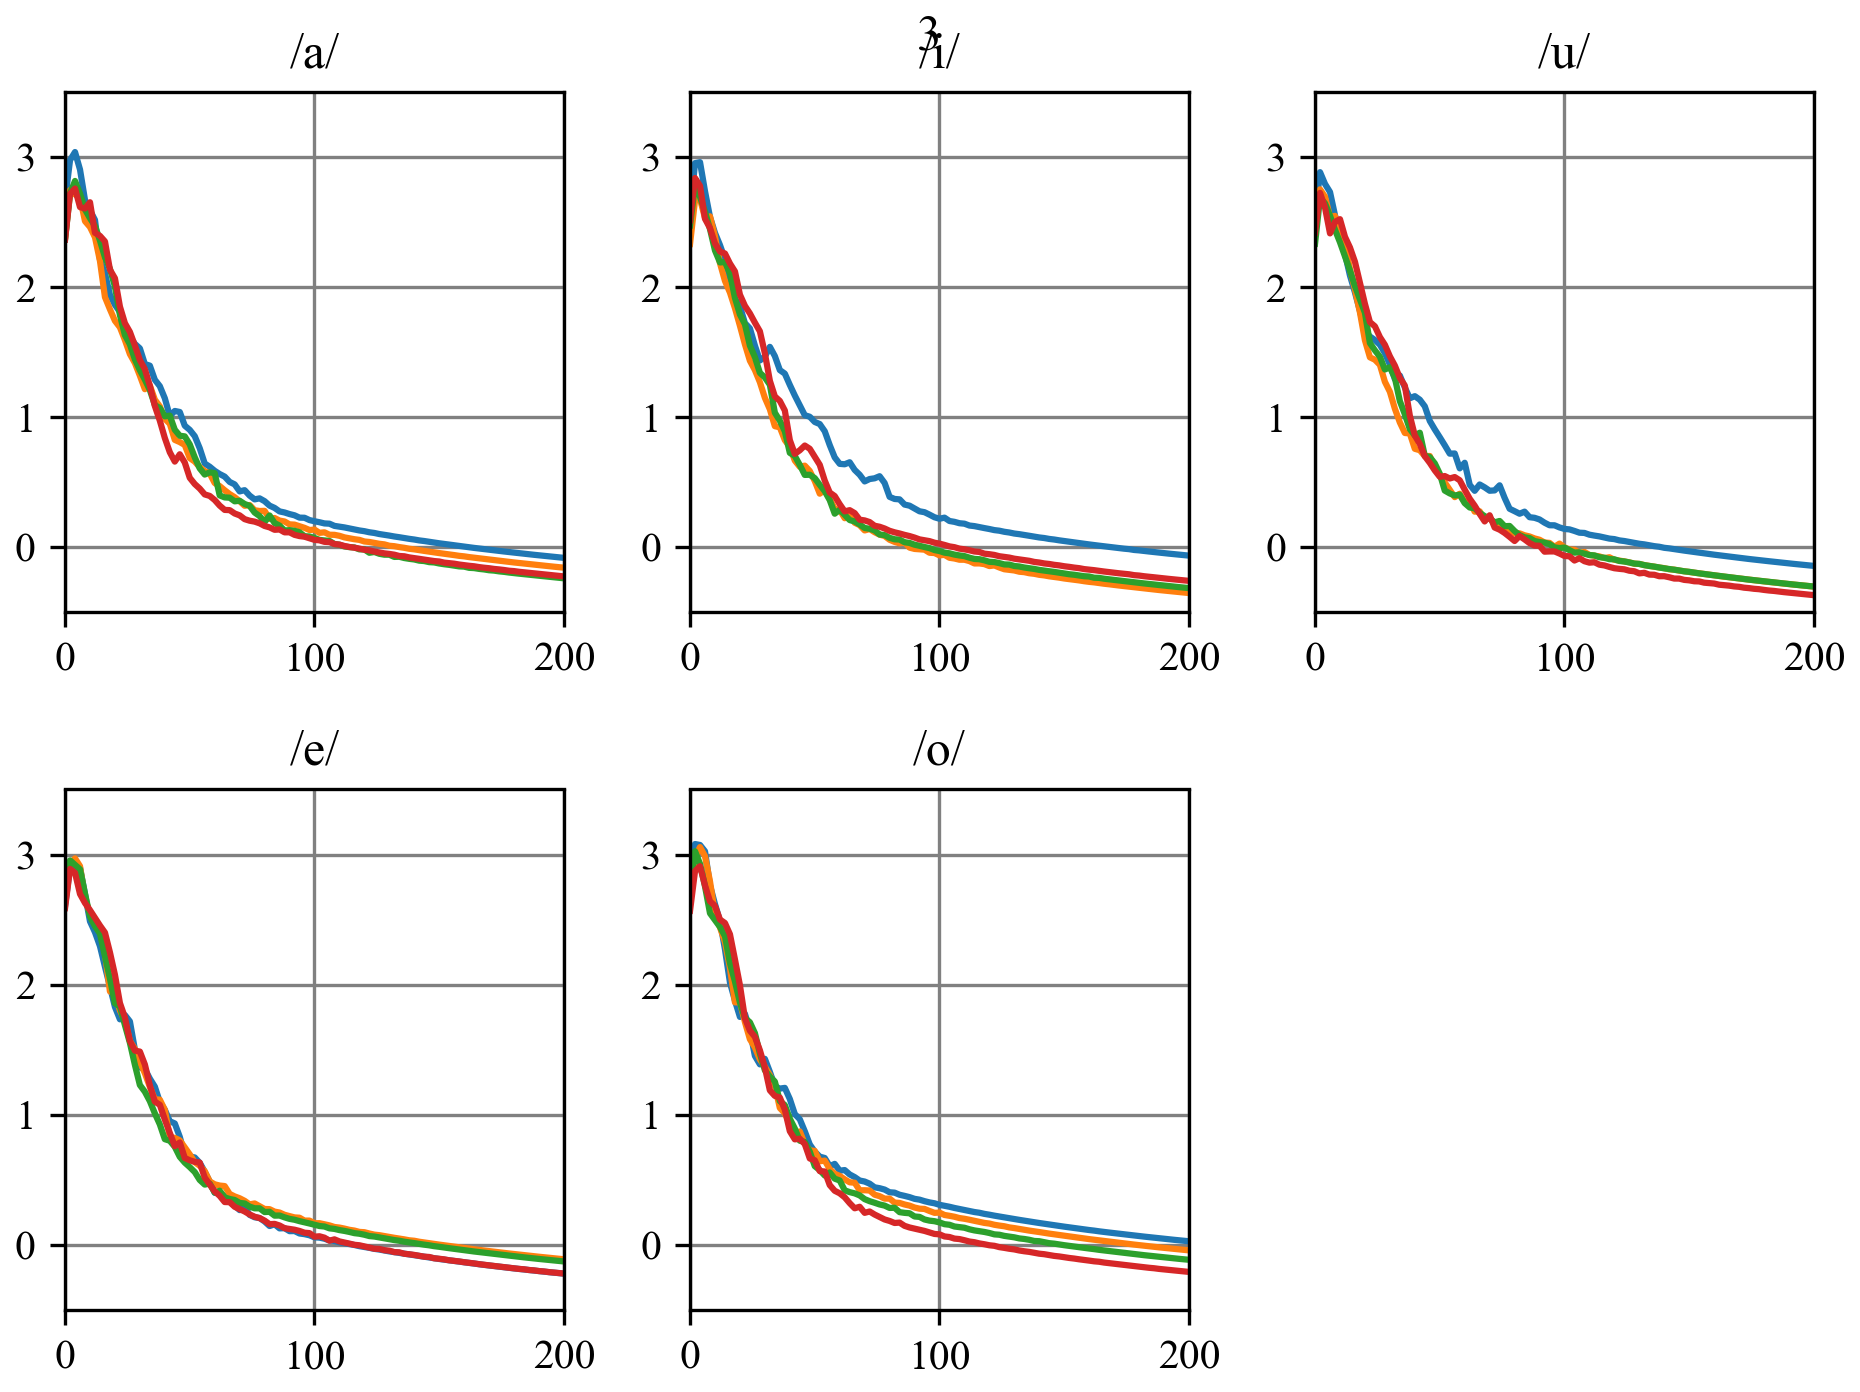
\includegraphics[clip,width=12.0cm]{long_spectrogram_3.png}
      \caption{被験者3のモジュレーションの全体平均}
      \label{long_spectrogram_3}
    \end{center}
\end{figure}

\begin{figure}[htbp]
    \begin{center}
      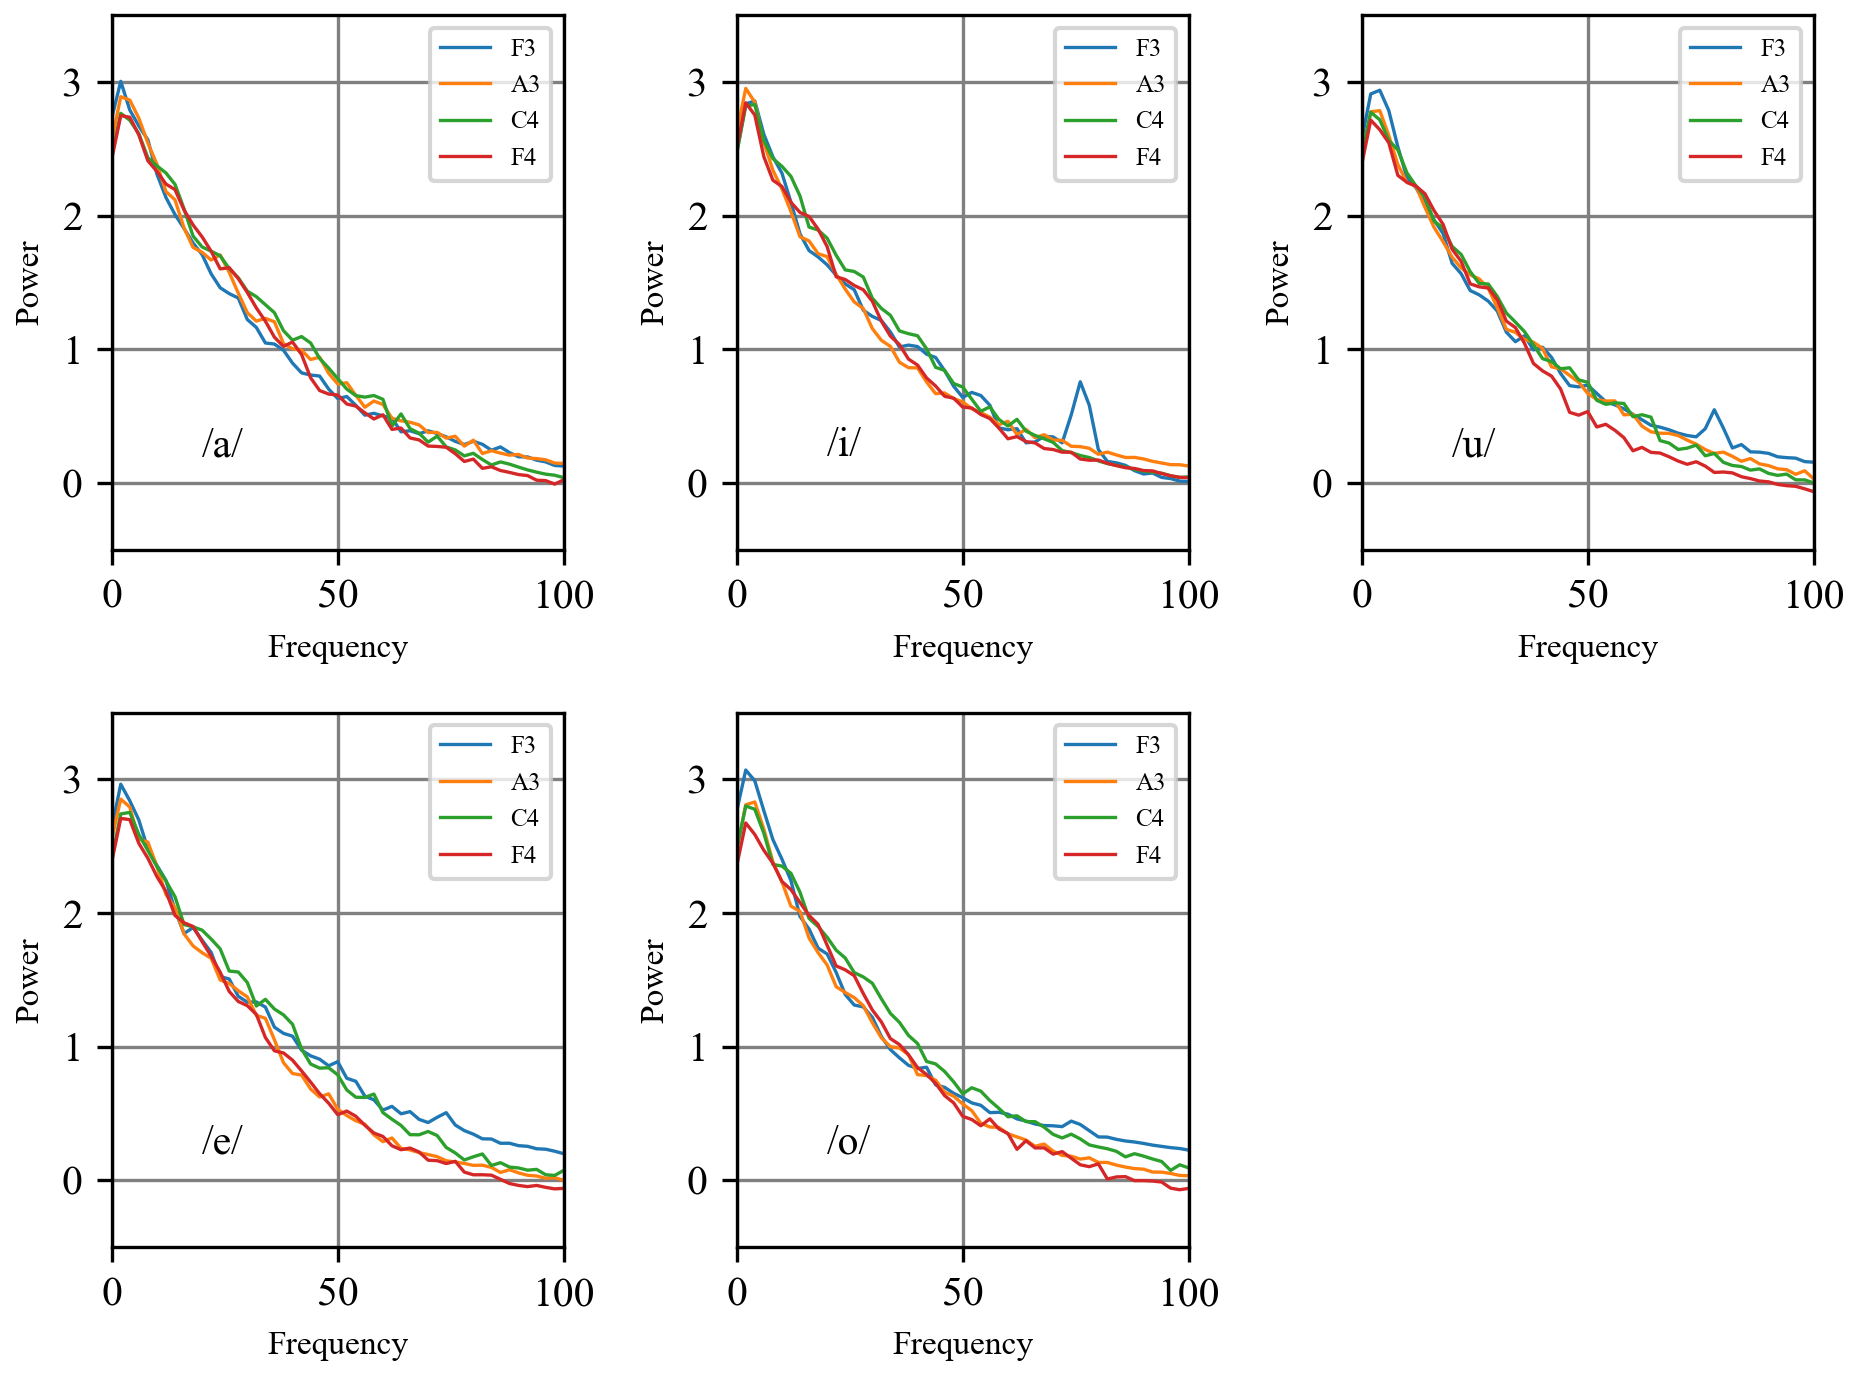
\includegraphics[clip,width=12.0cm]{long_spectrogram_4.png}
      \caption{被験者4のモジュレーションの全体平均}
      \label{long_spectrogram_4}
    \end{center}
\end{figure}



%---------------------------%

\chapter{結論}
\section{総括}
本研究では、音高・音色ごとの発声難度の分析による様々な応用を目指し、これを実現するために
被験者らの歌唱音声を収録して主に$F_0$に関する分析を行った。

\section{今後の課題}

音高・音色ごとの発声しにくさを分析するために4人の被験者からデータを収録したが、
個人性が強く全体に共通する特徴は多く見られなかった。
この個人性は歌唱経験の差や歌い方の癖で一定の傾向があると考えられるため、被験者数を増やして
同様の実験を行い、傾向ごとに発声難度の分析を行う必要がある。
また、収録は短時間に連続して行ったため、疲労による影響が生じていると考えられる。
十分な休憩を取るなどして各音ごとに出来る限り平等な条件で収録を行う必要がある。


また、それぞれの母音が正しいものとして議論を進めたが、実際は歌唱における母音の明瞭性の低下も考慮に入れる必要がある。
聴取実験を行い、母音の明瞭性や発声の客観的な評価を行う必要があると考えられる。

今回の収録は母音のみに限定しておりメロディもごく簡単なものであったため、
より音楽的な歌詞・メロディにおいても収録し、同様に分析を行う必要がある。


%---------------------------%

\chapter*{謝辞}
本研究を進めるにあたって、齋藤大輔講師には指導教員としてテーマをいただいたほか、研究を通して指導していただきました。深く感謝申し上げます。
峯松信明教授には、もう一人の指導教員として研究の方針について指導いただきました。深く感謝申し上げます。
峯松・齋藤研究室の先輩方にも様々な助言をいただきました。深く感謝申し上げます。
また、忙しい時期にもかかわらず実験に参加してくださった皆様のおかげで研究を進めることができました。深く感謝申し上げます。
最後に、私を支えてくれた家族と友人に深く感謝申し上げます。

\begin{flushright}
2020年2月7日

小林 海斗
\end{flushright}

\bibliography{references}


\appendix
\chapter{他被験者の収録データ}

\begin{figure}[htbp]
    \begin{center}
      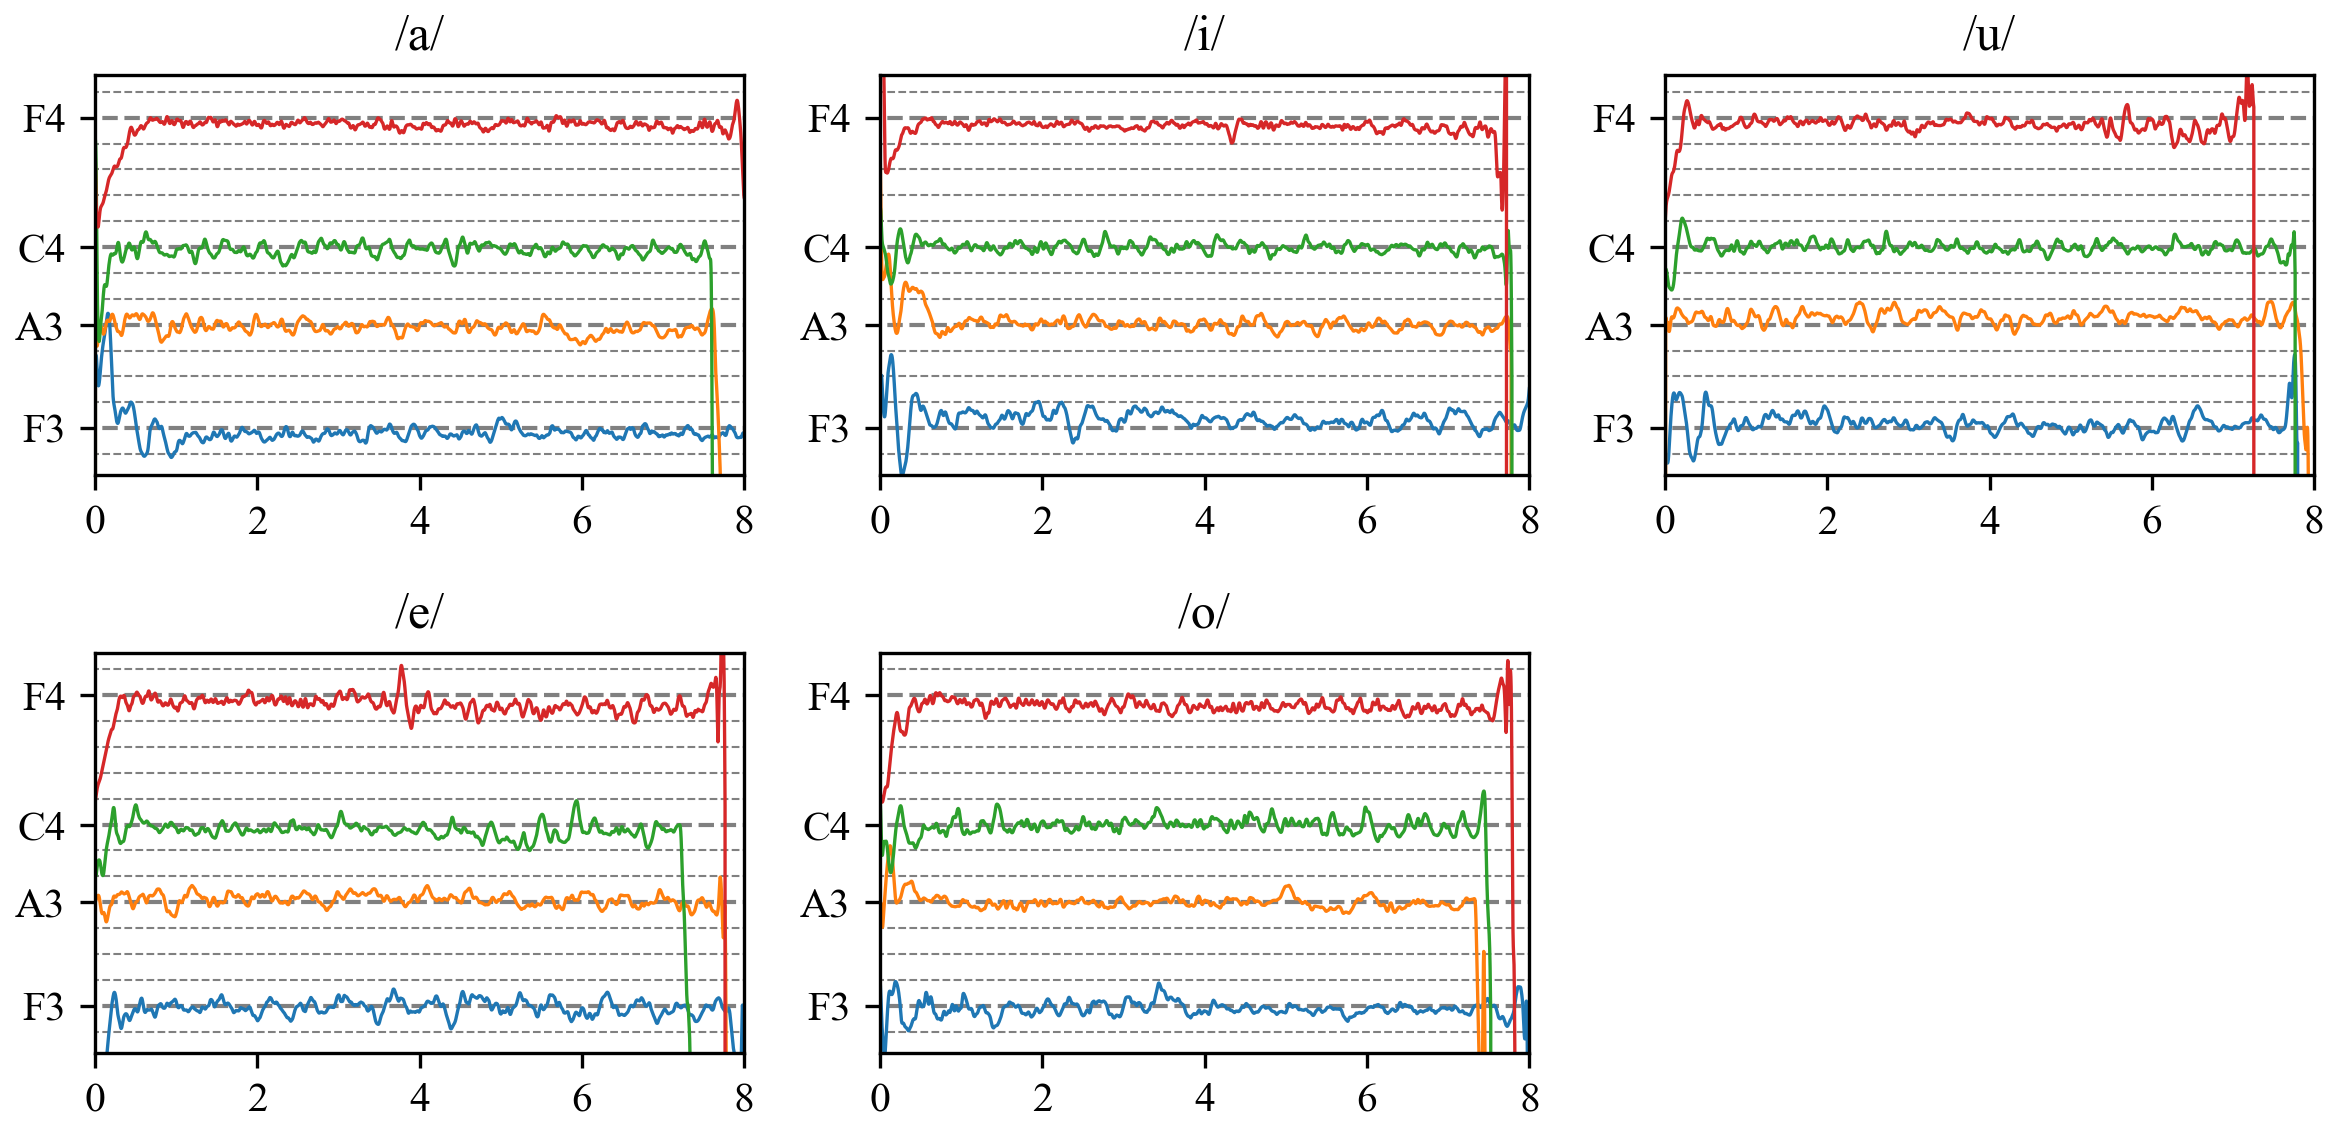
\includegraphics[clip,width=16.0cm]{F0_long_2.png}
      \caption{被験者2の単音発声}
      \label{fig:2}
    \end{center}
\end{figure}

\begin{figure}[htbp]
    \begin{center}
      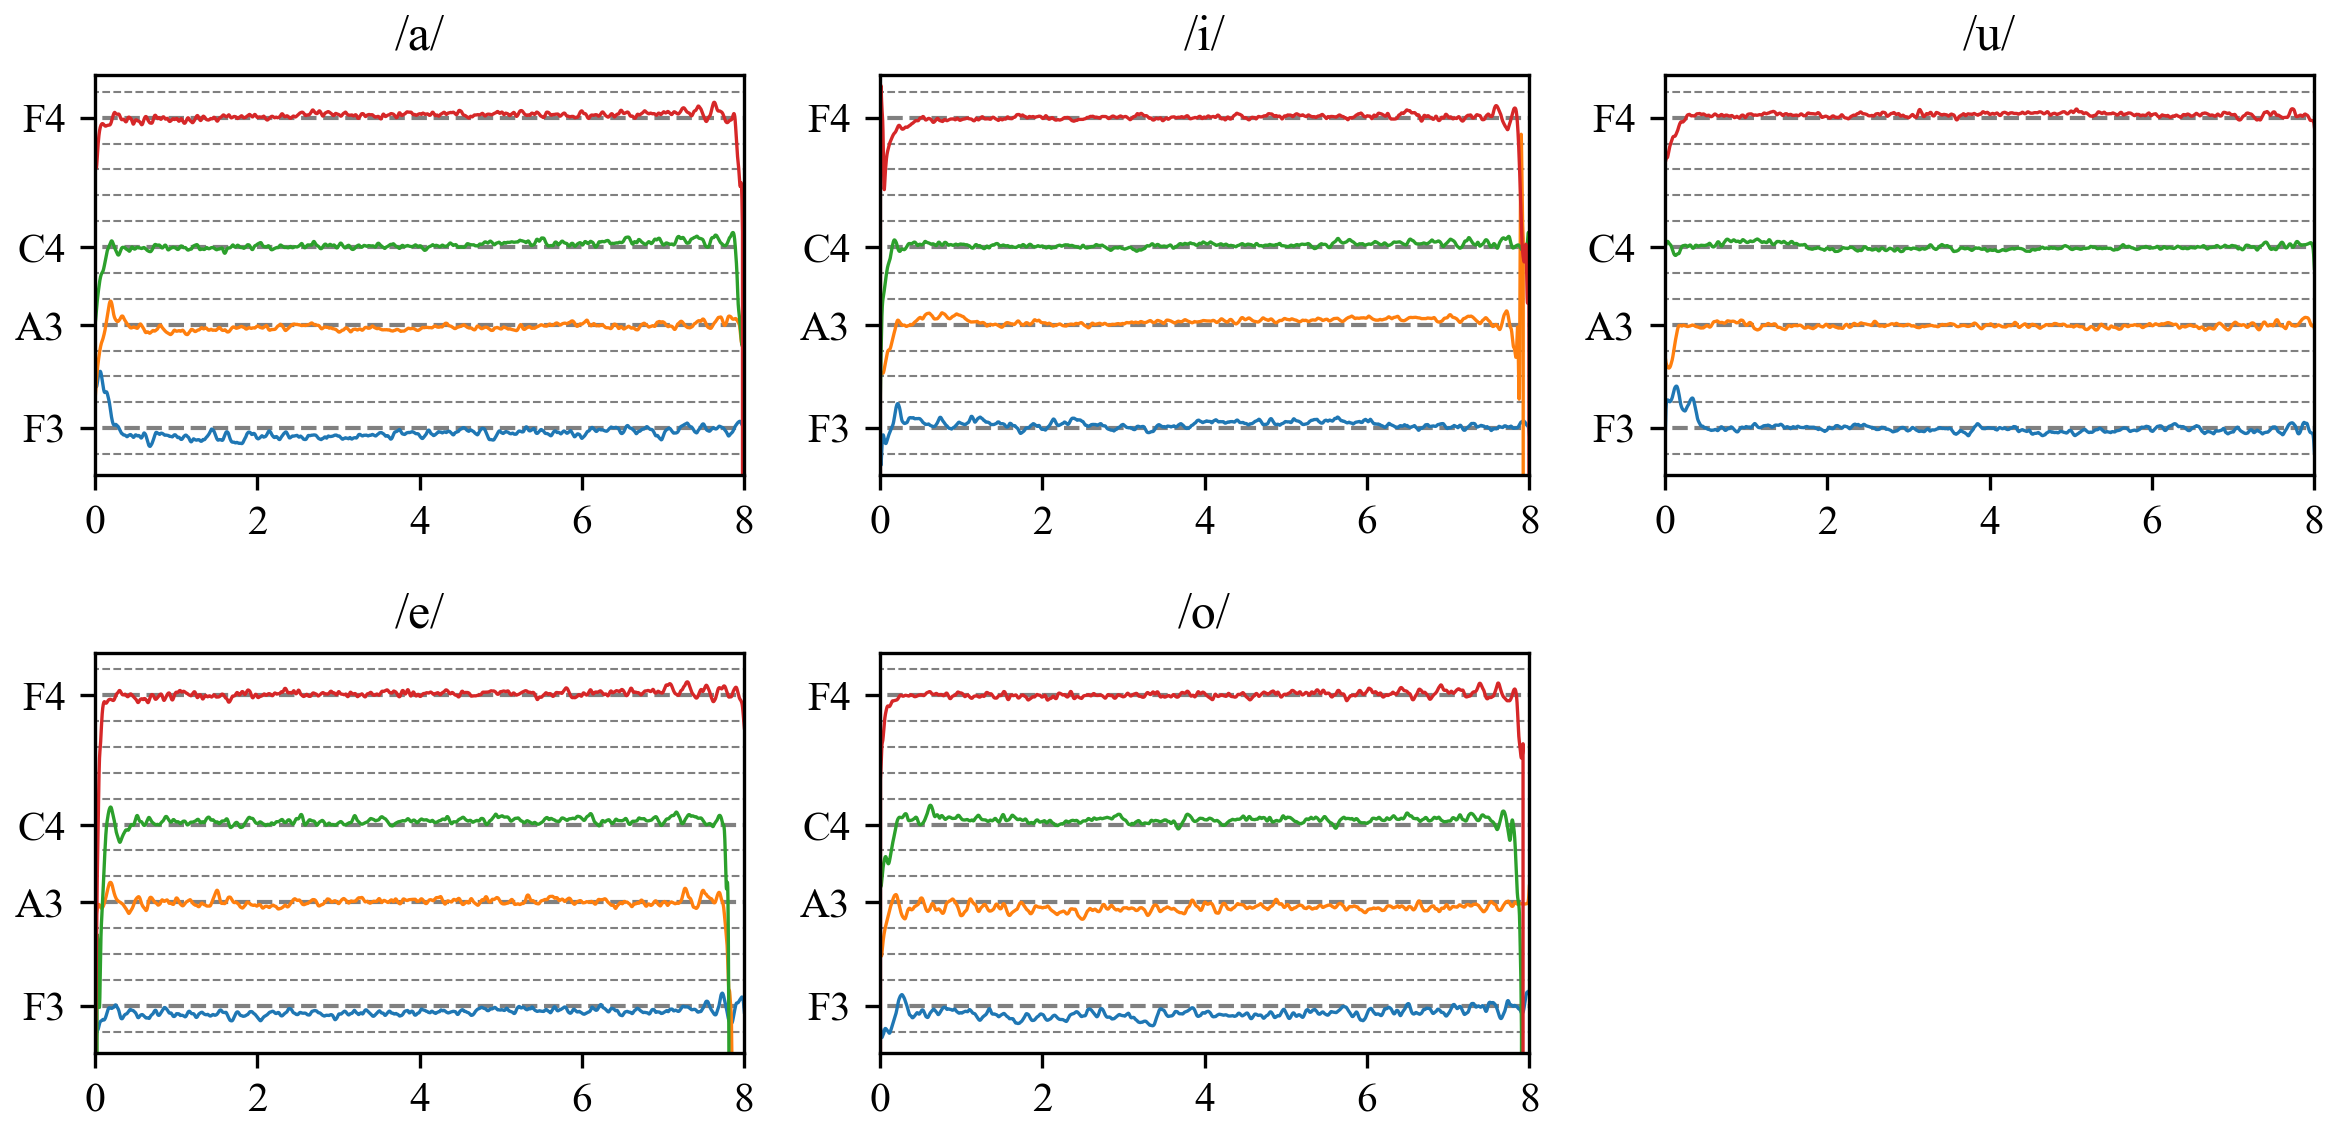
\includegraphics[clip,width=16.0cm]{F0_long_3.png}
      \caption{被験者3の単音発声}
      \label{fig:3}
    \end{center}

\end{figure}

\begin{figure}[htbp]
    \begin{center}
      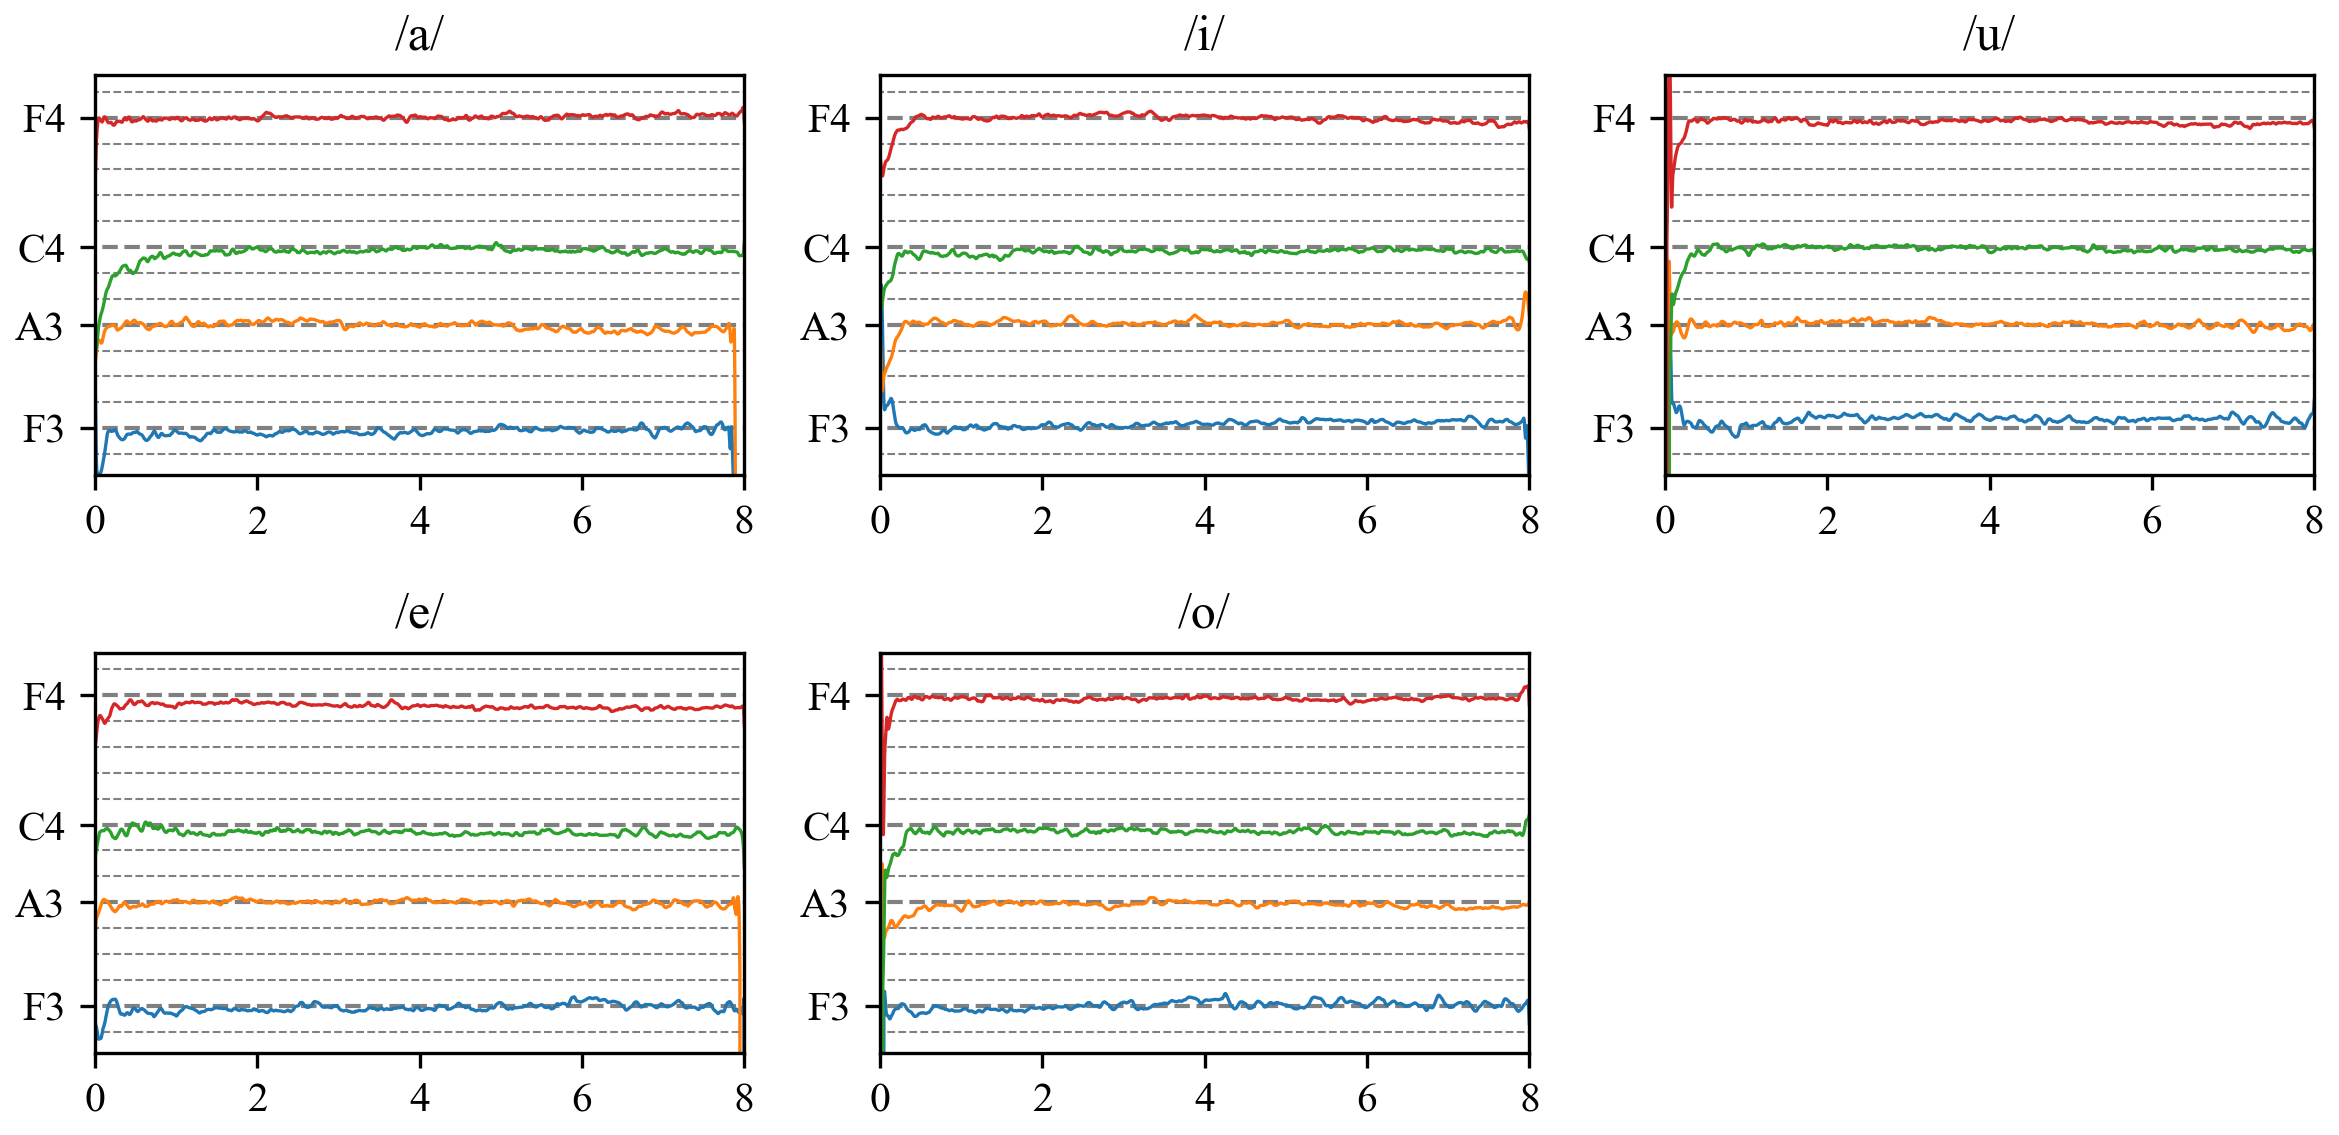
\includegraphics[clip,width=16.0cm]{F0_long_4.png}
      \caption{被験者4の単音発声}
      \label{fig:4}
    \end{center}
\end{figure}





\begin{figure}[htbp]
    \begin{center}
      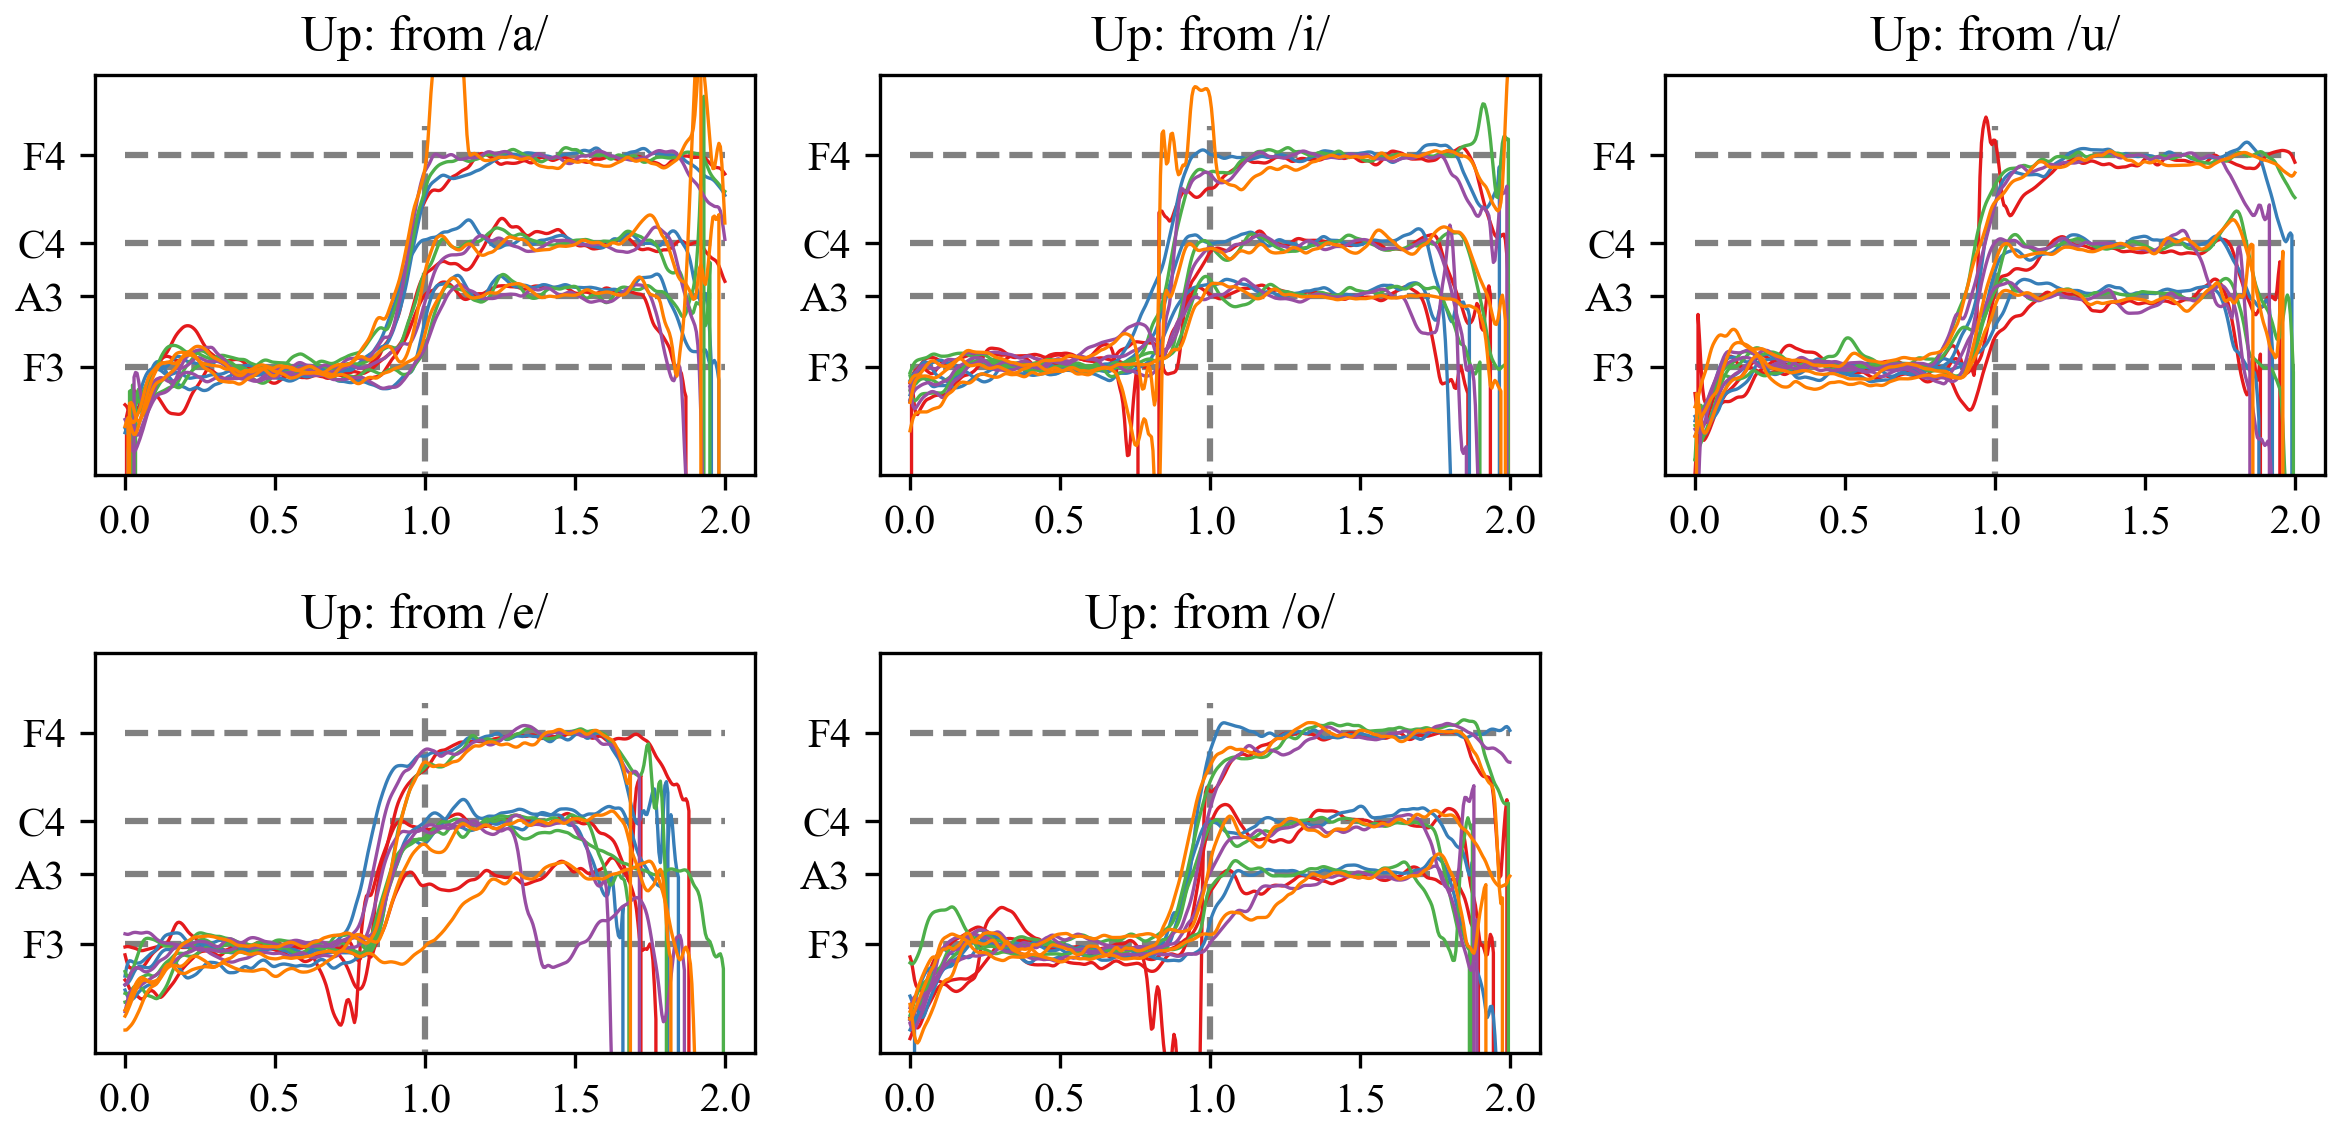
\includegraphics[clip,width=16.0cm]{F0_up_2.png}
      \caption{被験者2の上昇発声}
      \label{fig:u2}
    \end{center}
\end{figure}

\begin{figure}[htbp]
    \begin{center}
      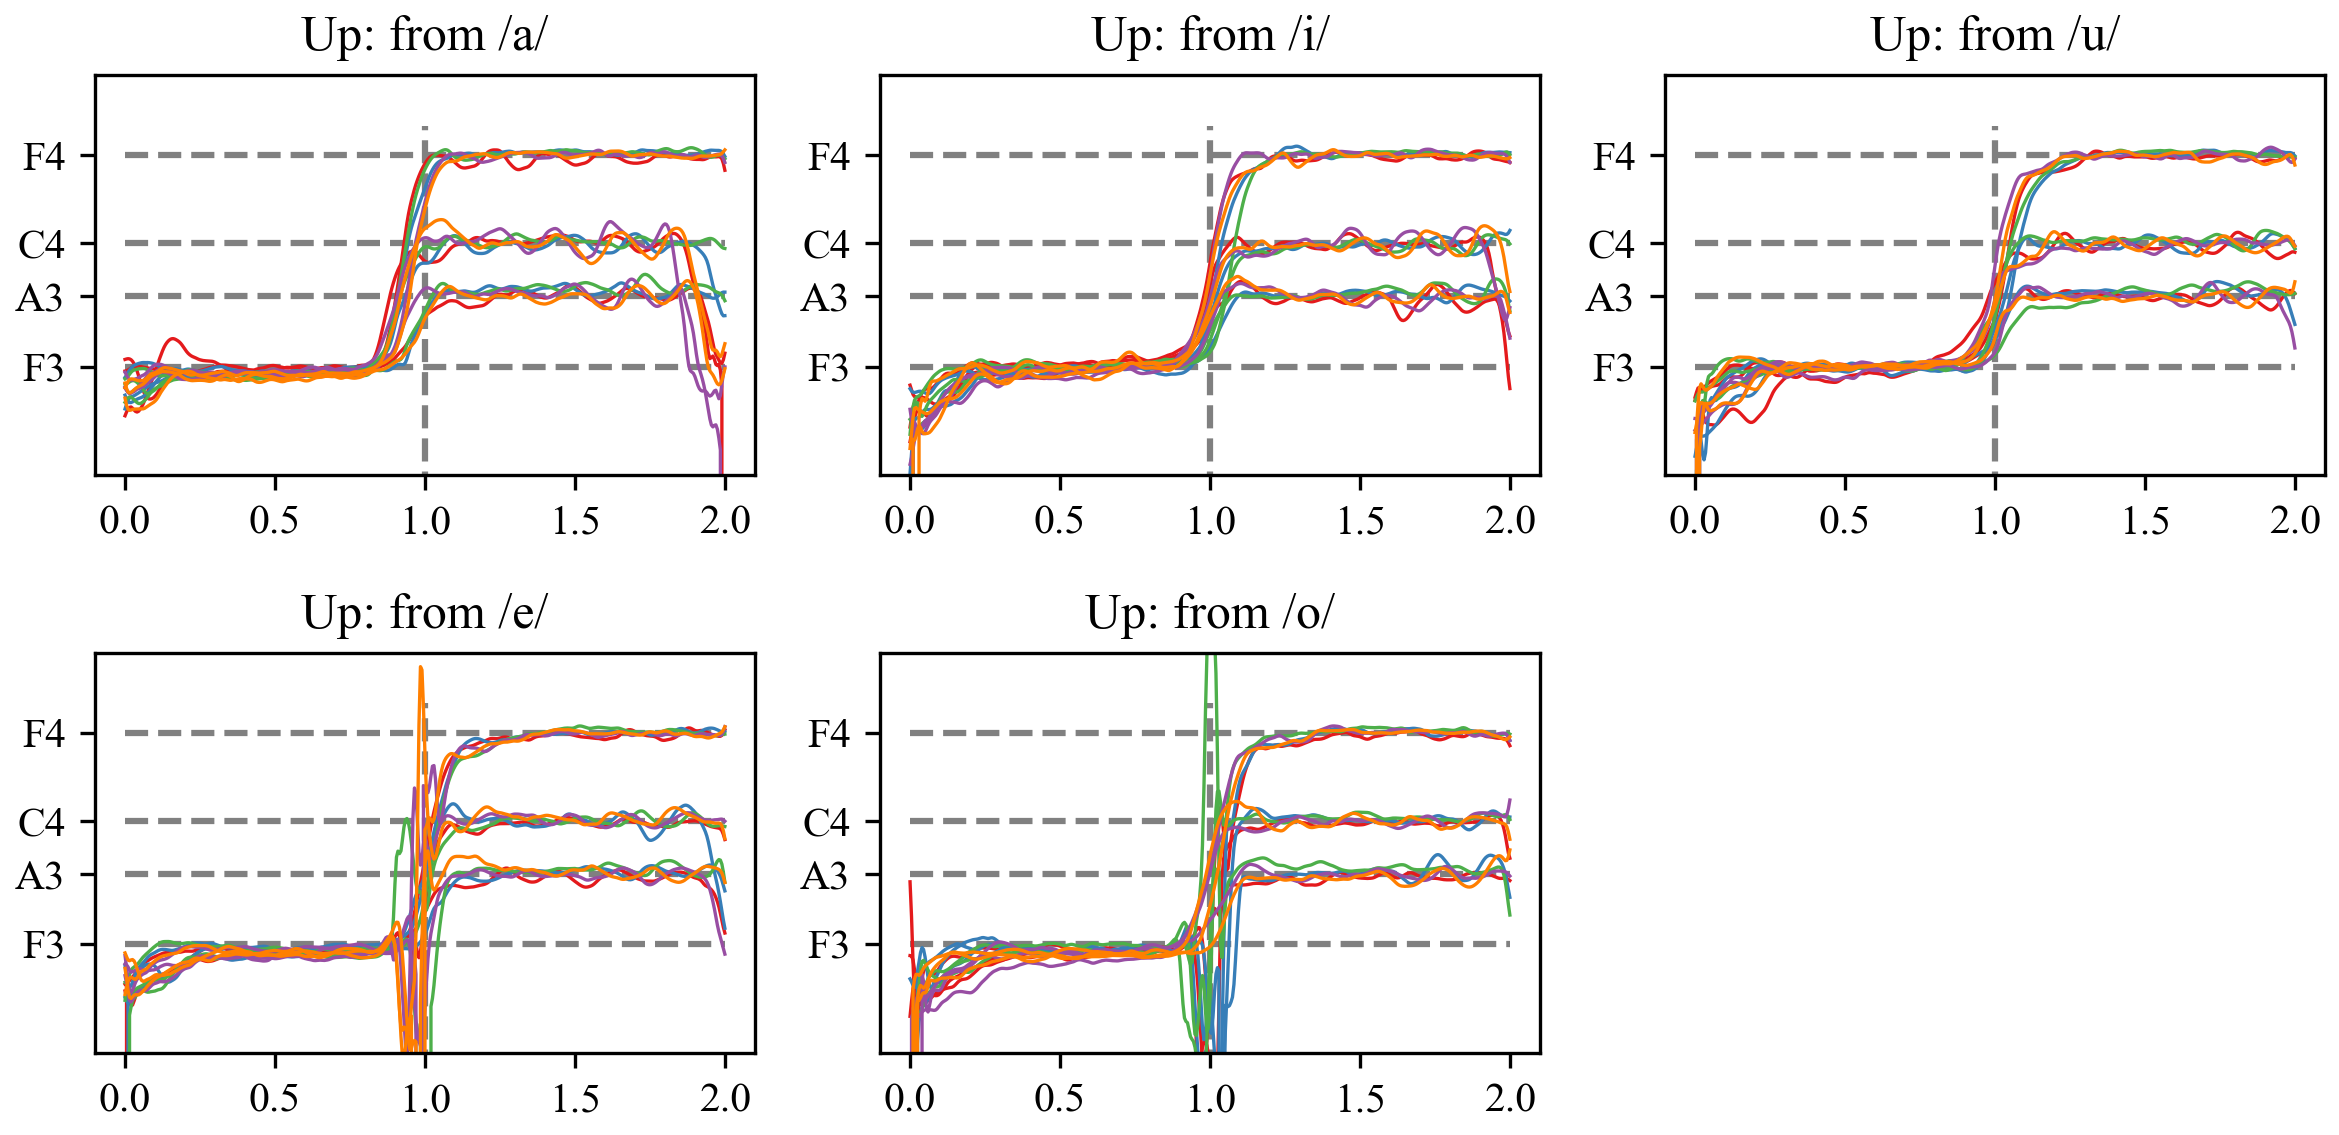
\includegraphics[clip,width=16.0cm]{F0_up_3.png}
      \caption{被験者3の上昇発声}
      \label{fig:u3}
    \end{center}

\end{figure}\begin{figure}[htbp]
    \begin{center}
      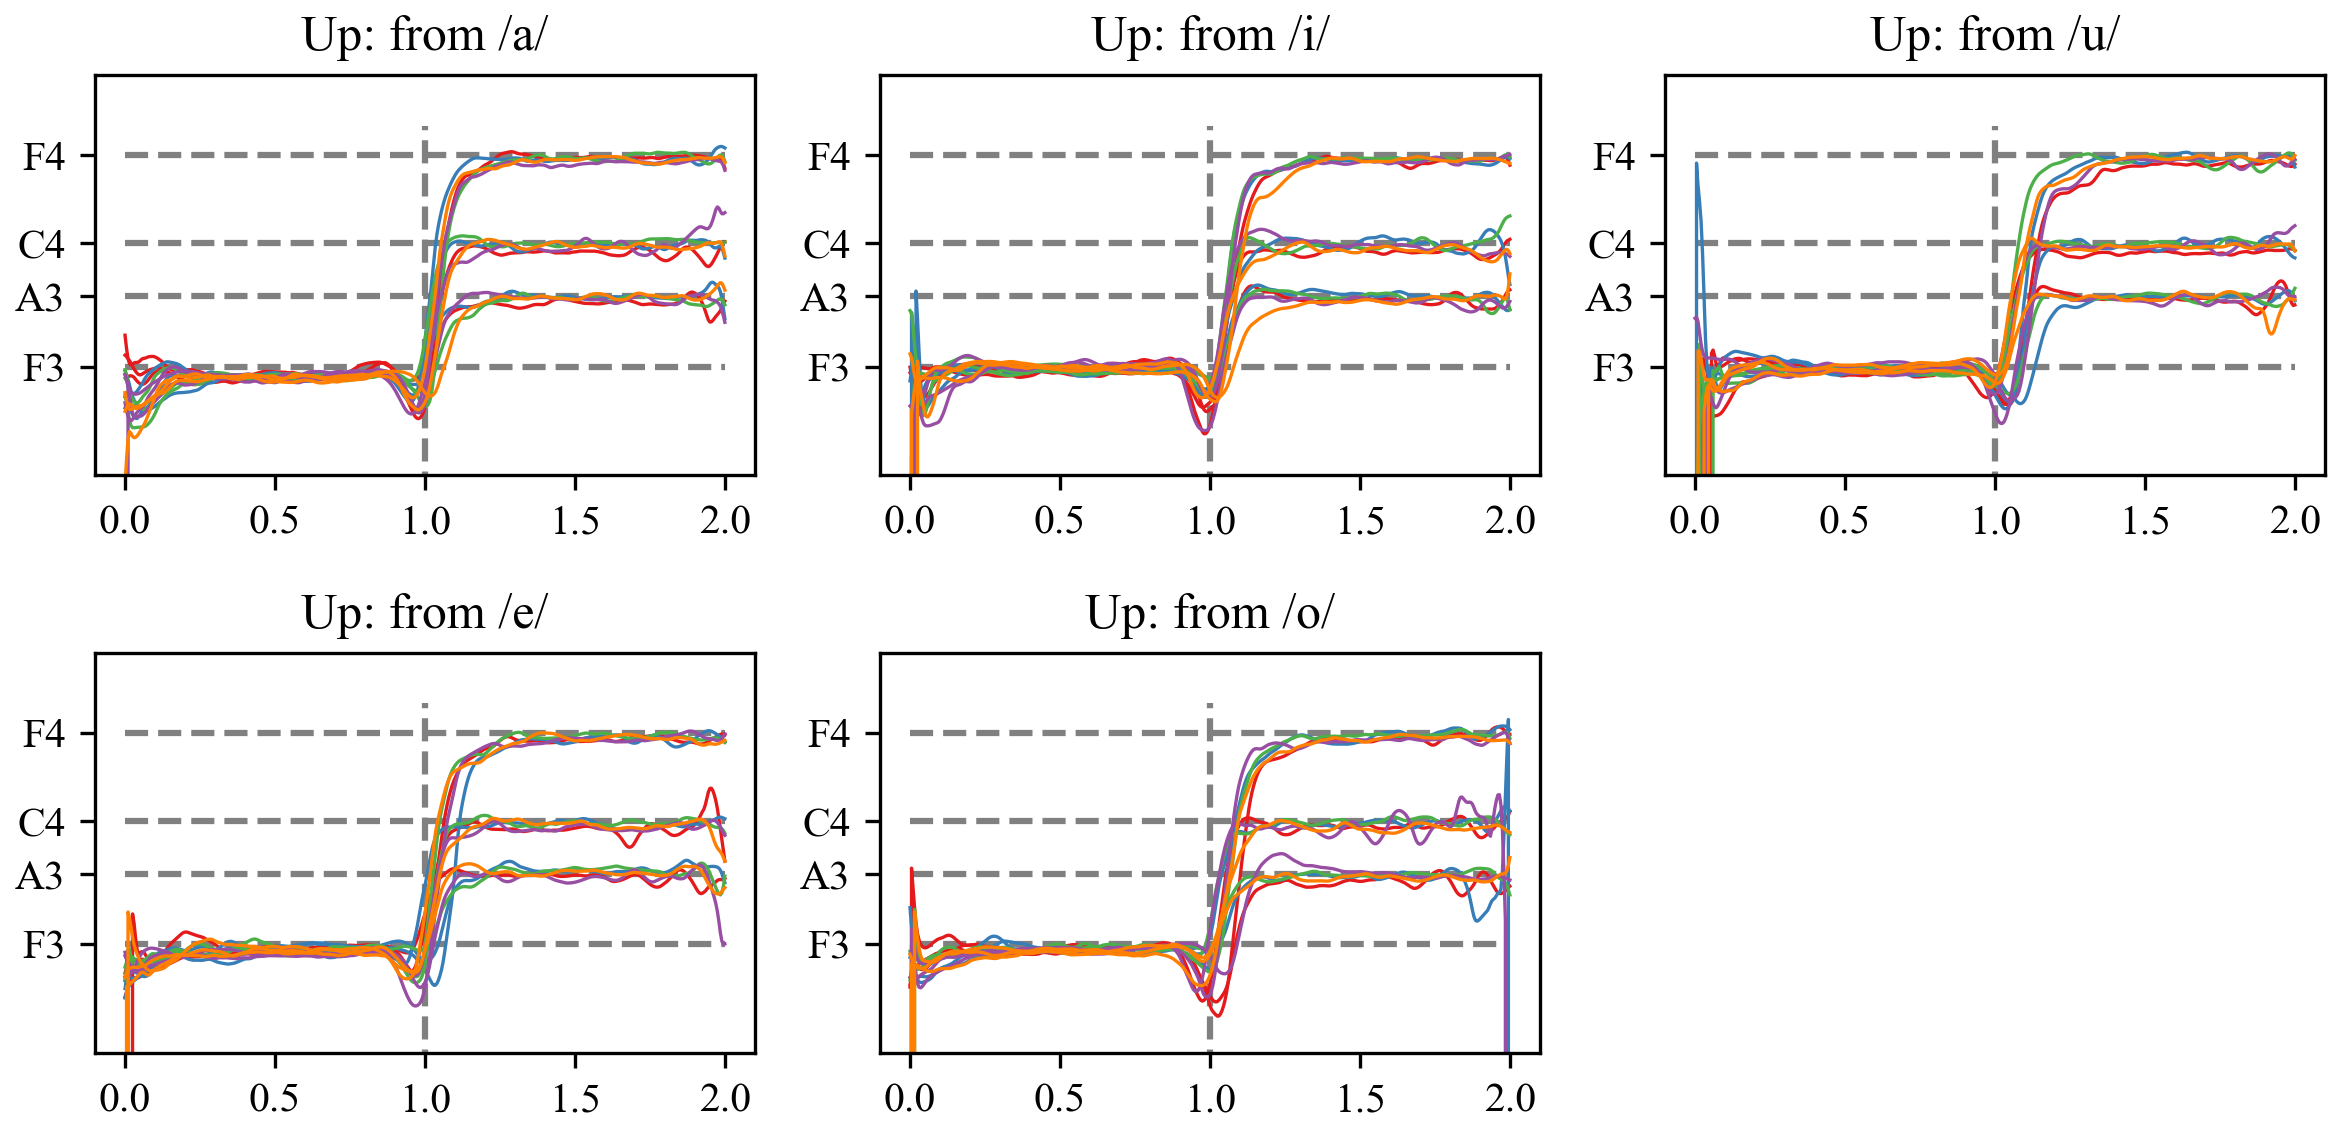
\includegraphics[clip,width=16.0cm]{F0_up_4.png}
      \caption{被験者4の上昇発声}
      \label{fig:u4}
    \end{center}
\end{figure}





\begin{figure}[htbp]
    \begin{center}
      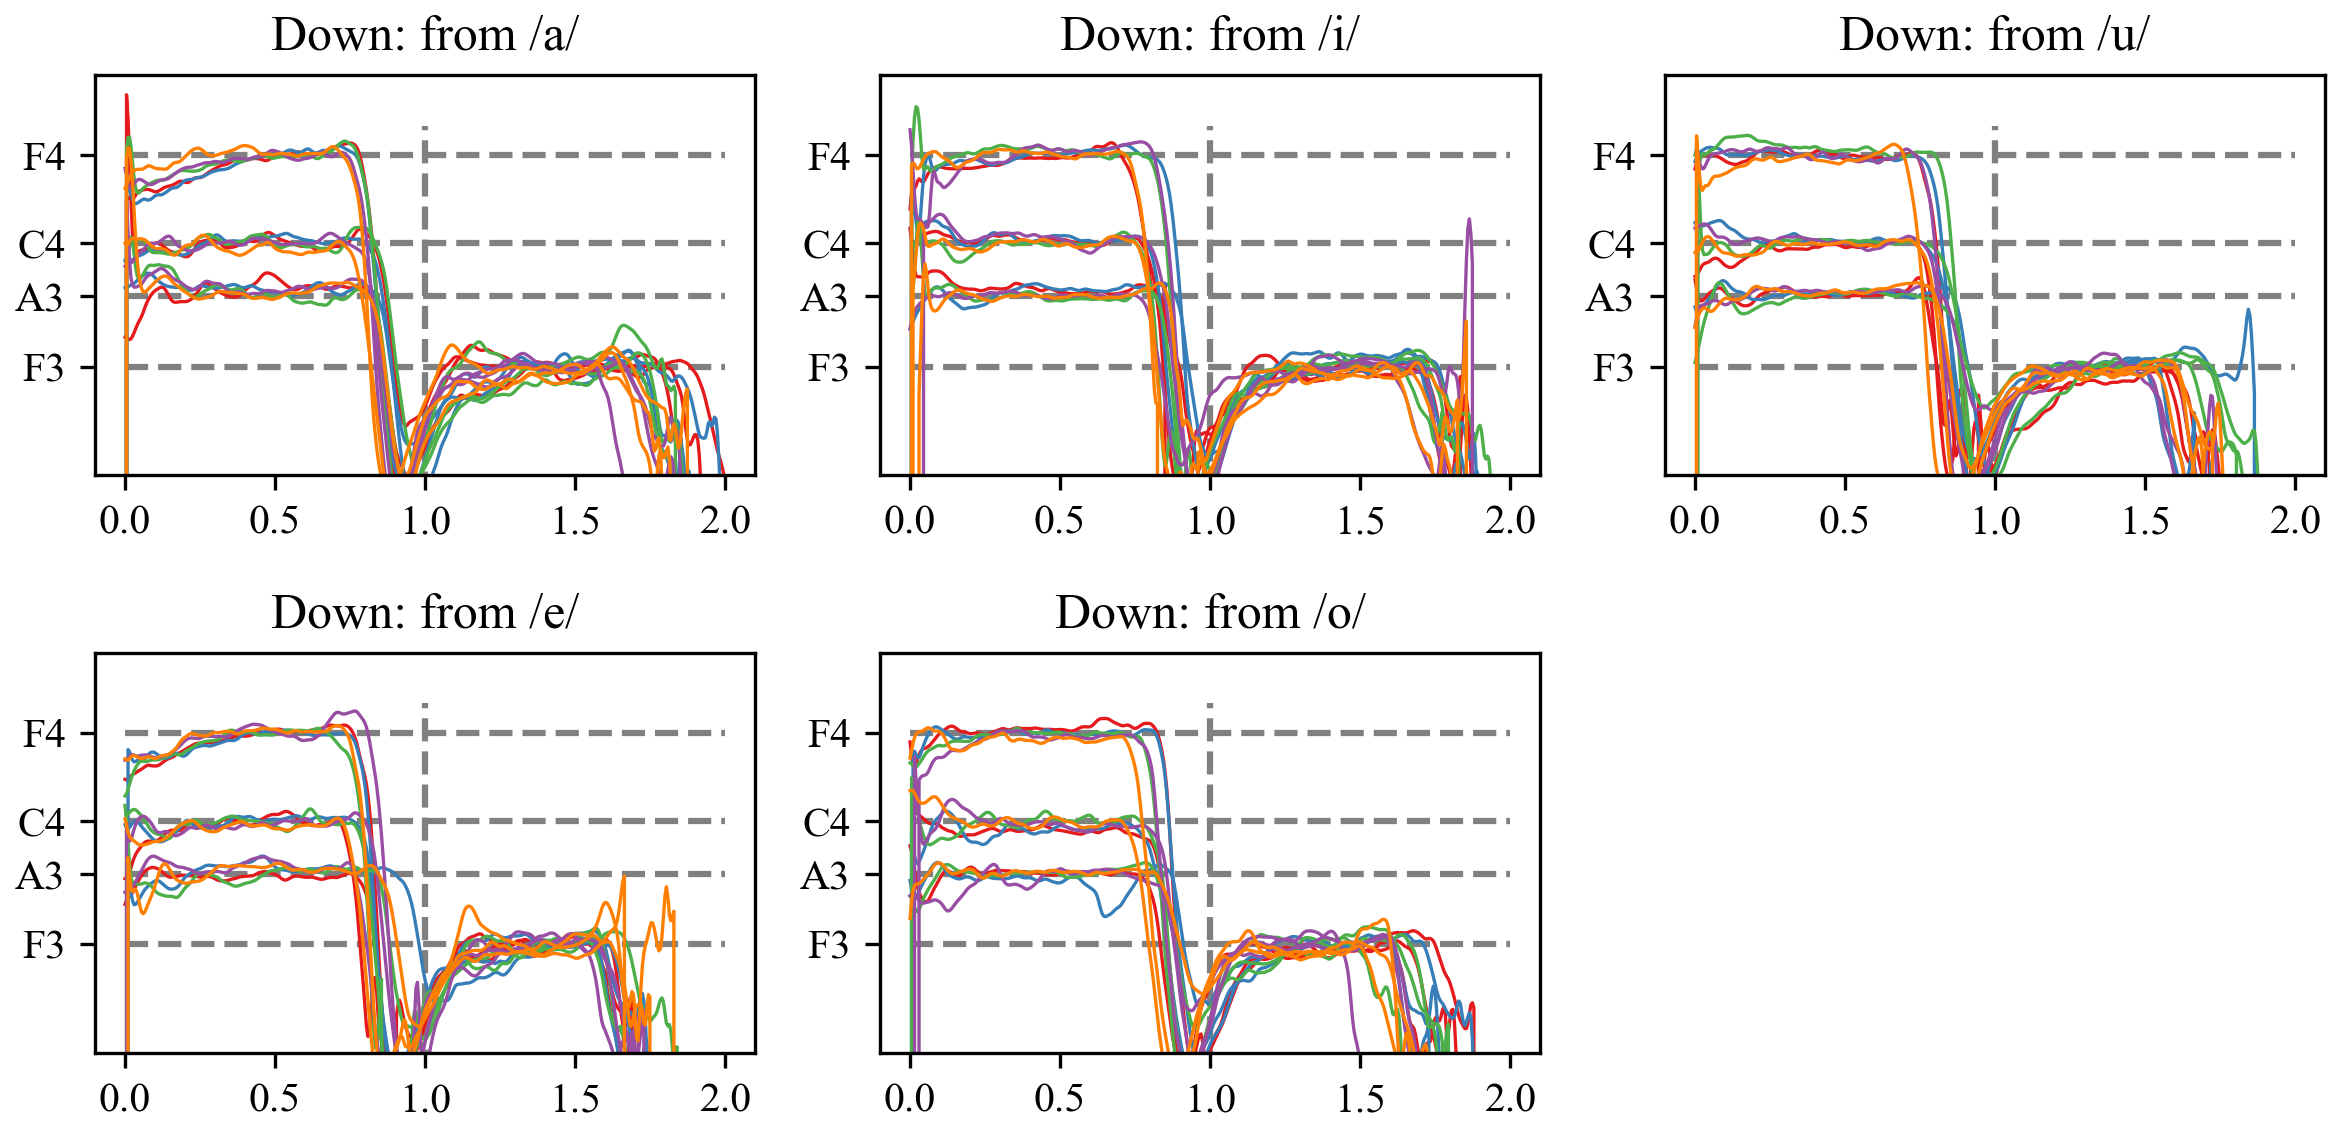
\includegraphics[clip,width=16.0cm]{F0_down_2.png}
      \caption{被験者2の下降発声}
      \label{fig:d2}
    \end{center}
\end{figure}

\begin{figure}[htbp]
    \begin{center}
      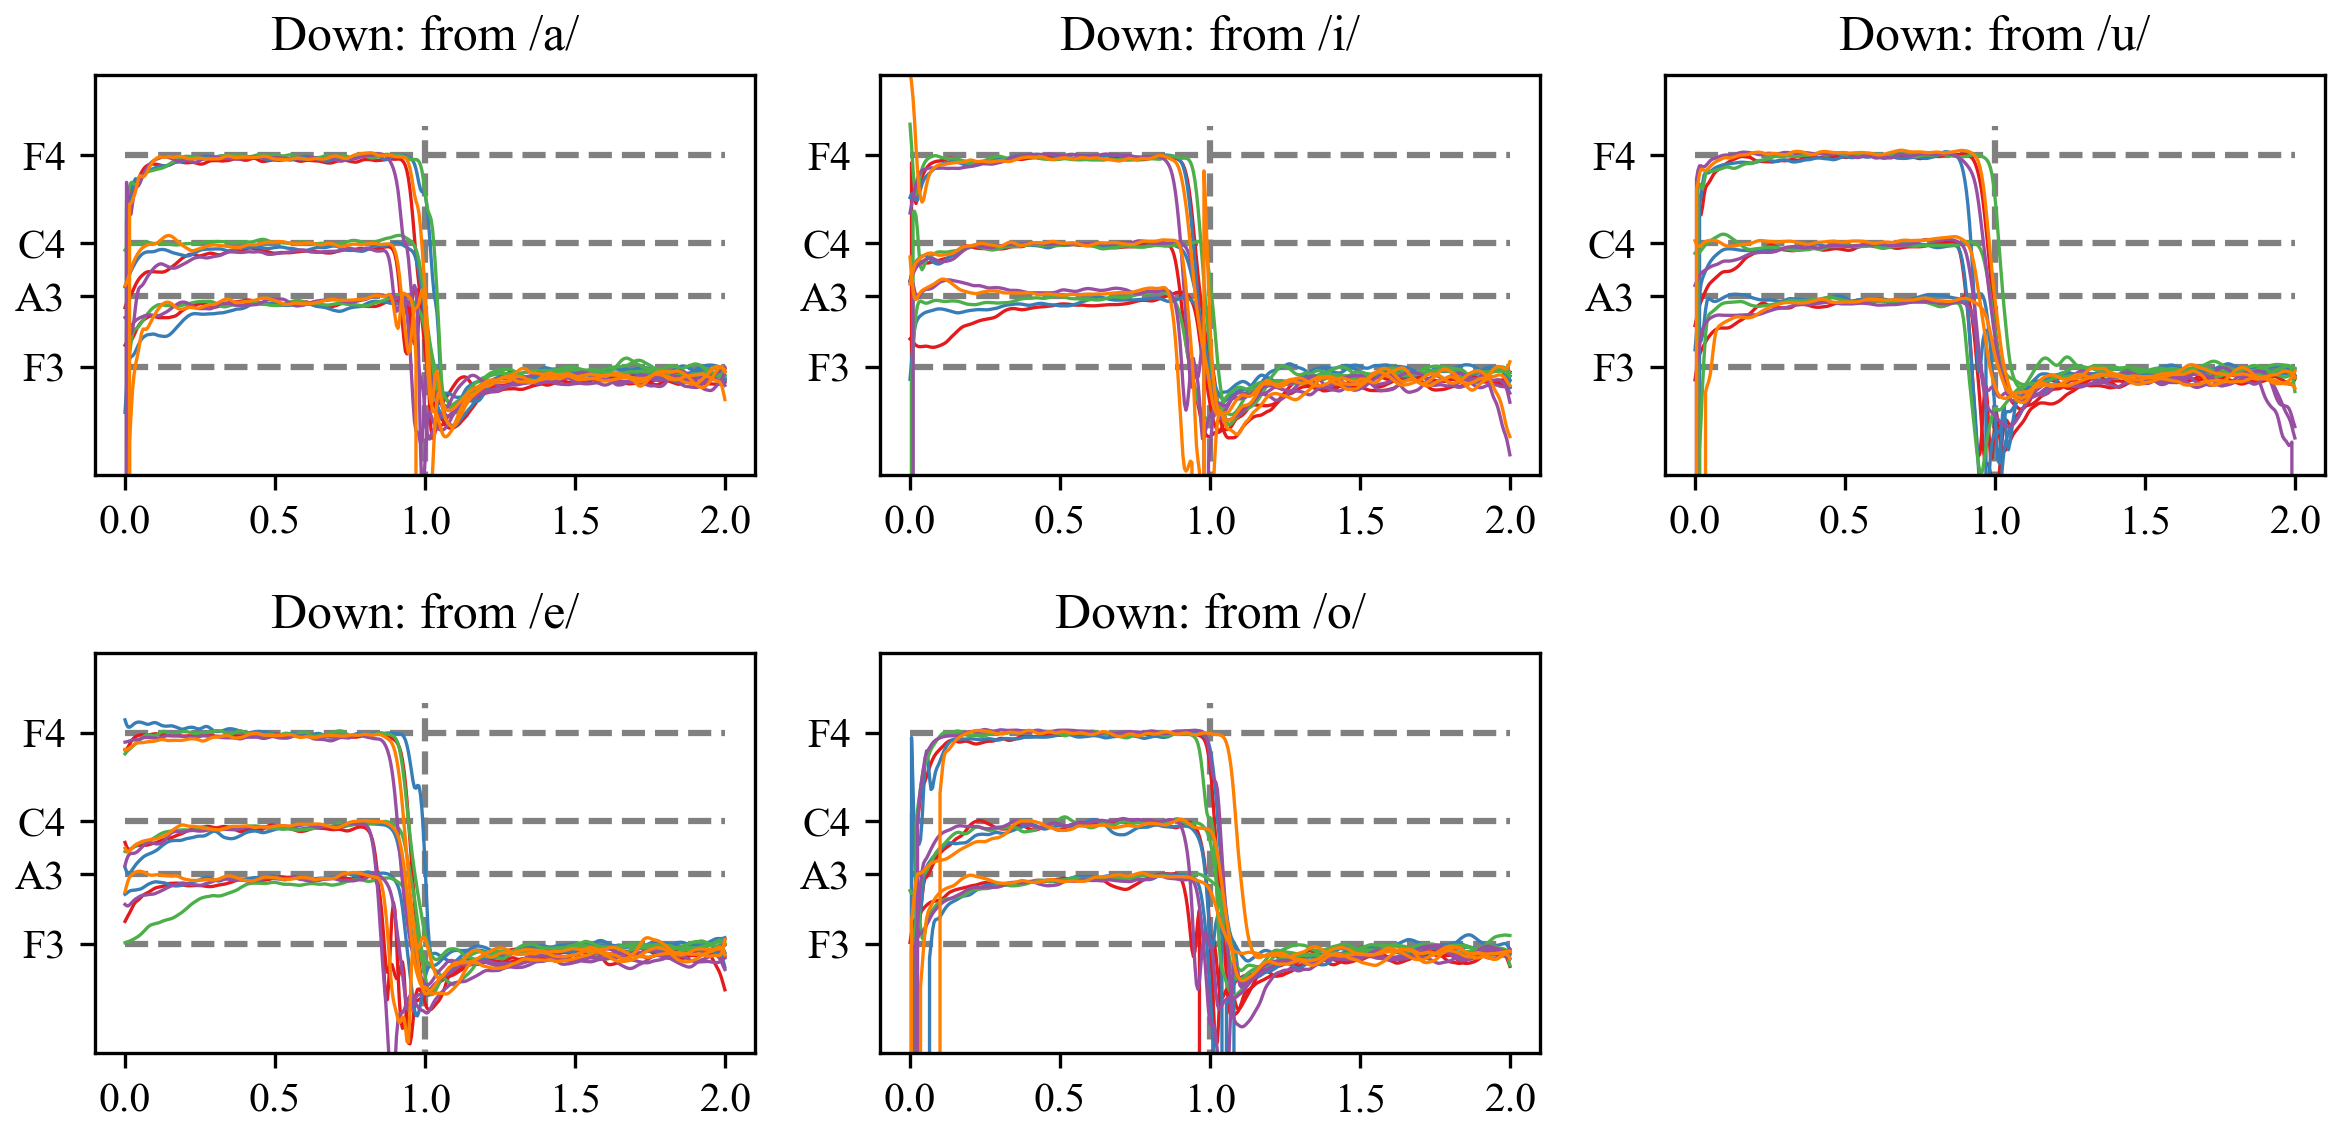
\includegraphics[clip,width=16.0cm]{F0_down_3.png}
      \caption{被験者3の下降発声}
      \label{fig:d3}
    \end{center}

\end{figure}\begin{figure}[htbp]
    \begin{center}
      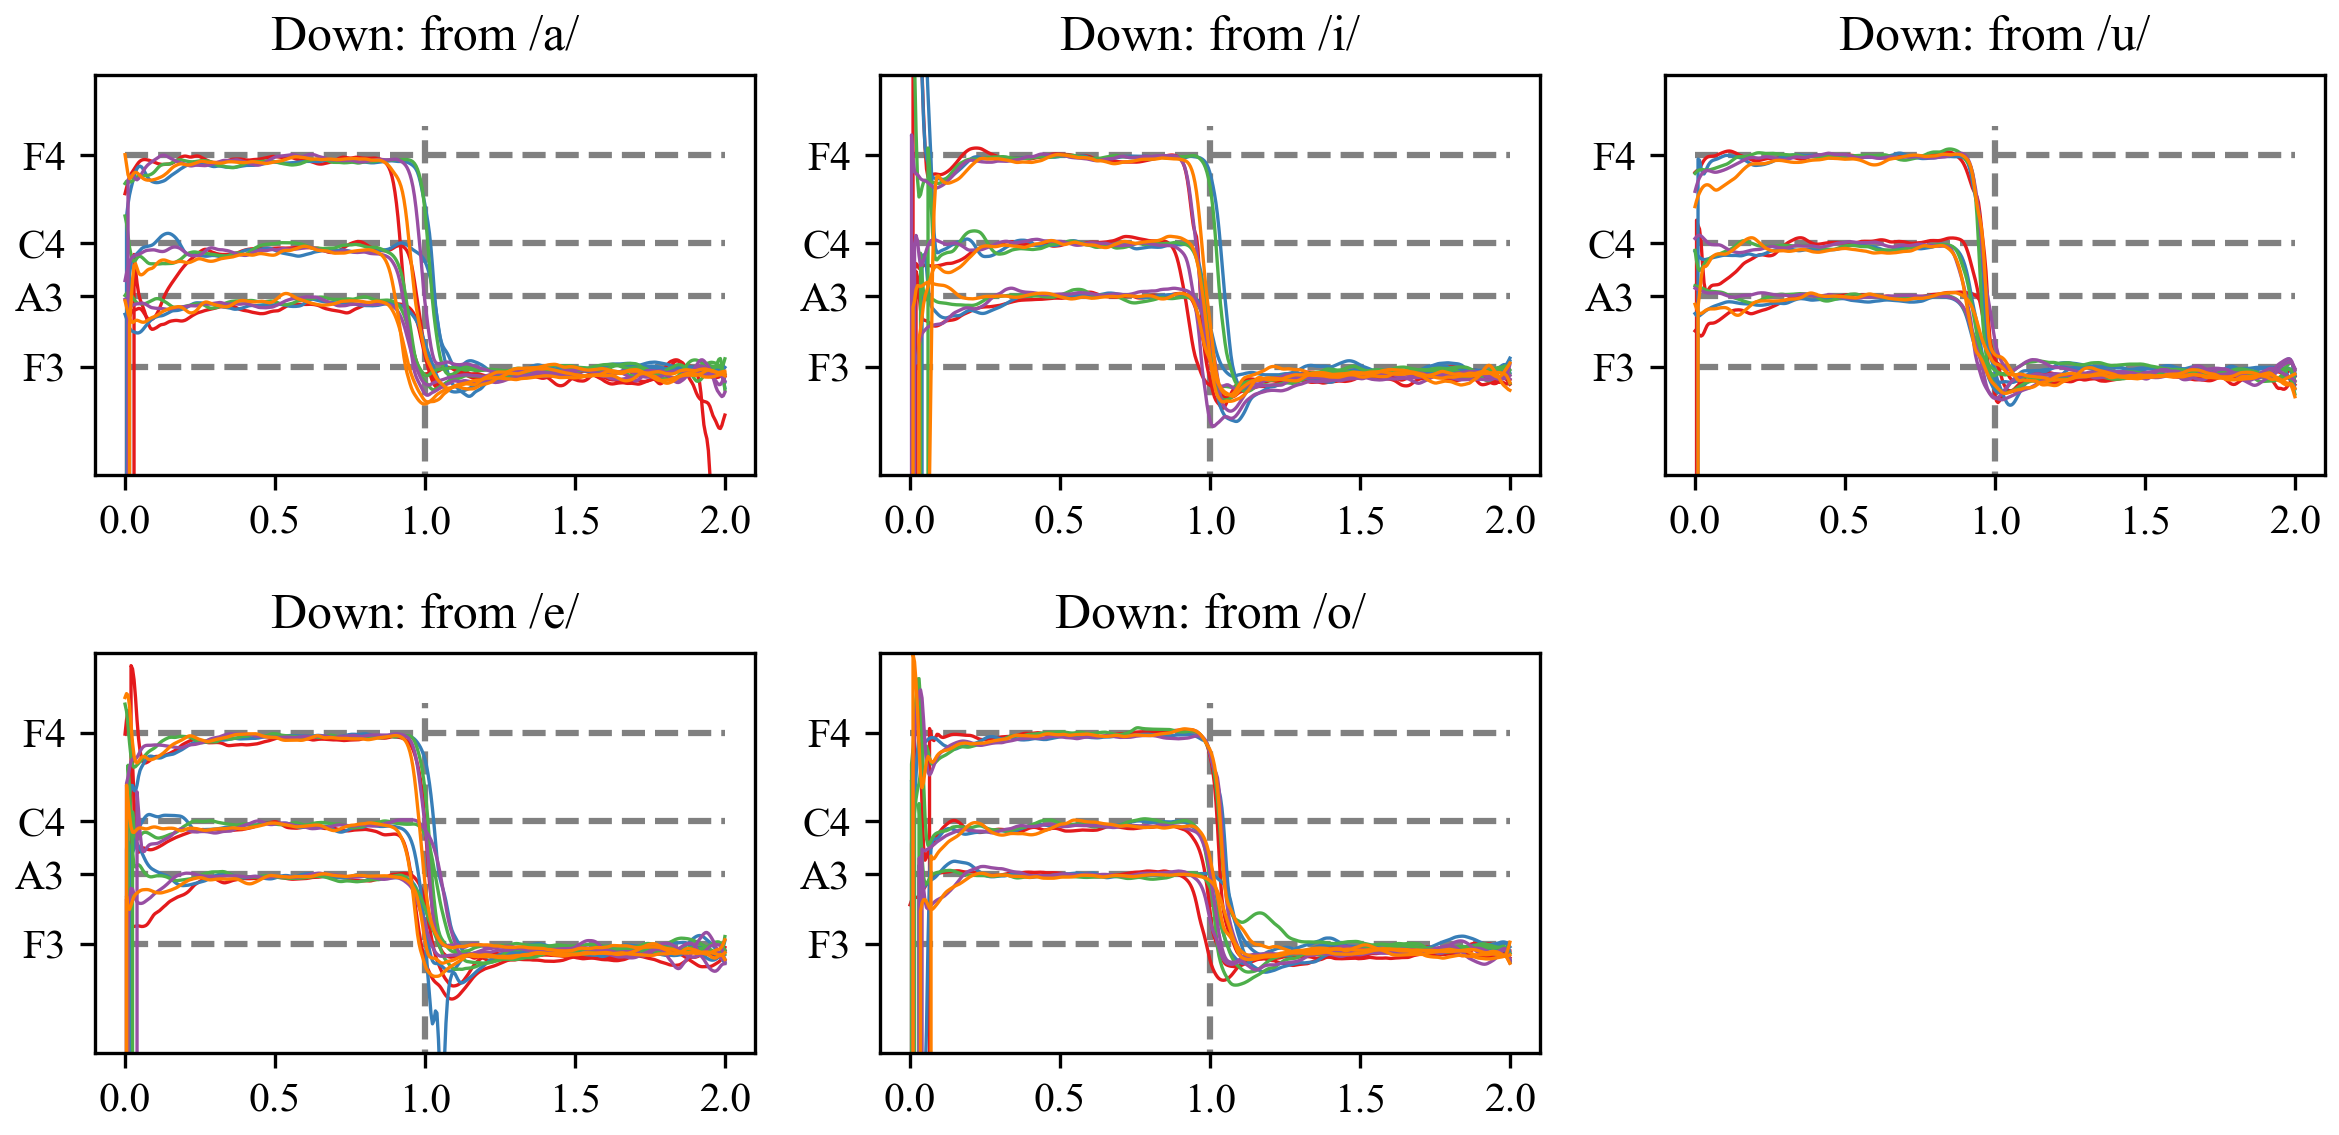
\includegraphics[clip,width=16.0cm]{F0_down_4.png}
      \caption{被験者4の下降発声}
      \label{fig:d4}
    \end{center}
\end{figure}


\end{document}